\documentclass{article}

\addtolength{\oddsidemargin}{-.875in}
\addtolength{\evensidemargin}{-.875in}
\addtolength{\textwidth}{1.75in}
\addtolength{\topmargin}{-.875in}
\addtolength{\textheight}{1.75in}

\usepackage{amssymb, amsthm, amstext, amsxtra, amsmath, amsfonts, amscd }
\usepackage{graphicx, epsfig, apacite, dirtytalk, fancyhdr}
\usepackage{comment, color, cleveref, listings, wrapfig}
 

\pagestyle{fancy}
\fancyhf{}
\fancyhead[L]{Bayesian Data Analysis}
\fancyhead[R]{ \leftmark}
\fancyfoot[C]{\thepage}

\definecolor{dkgreen}{rgb}{0,0.6,0}
\definecolor{gray}{rgb}{0.5,0.5,0.5}
\definecolor{mauve}{rgb}{0.58,0,0.82}
\definecolor{backcolour}{rgb}{0.95,0.95,0.92}


\lstdefinestyle{R}{frame=tb, backgroundcolor=\color{backcolour}, 
				   language=R, 
				   aboveskip=3mm, belowskip=3mm, 
				   showstringspaces=false,
				   columns=flexible, numbers=none, tabsize=3,
				   keywordstyle=\color{blue}, 
				   numberstyle=\tiny\color{gray}, 
				   commentstyle=\color{dkgreen},
				   stringstyle=\color{mauve}, 
				   breaklines=true, 
				   breakatwhitespace=true}
\lstset{style=R}

\def\E{\mathbb{E}}
\def\pr{\mathbb{P}}
\renewcommand\baselinestretch{1.2}

\DeclareMathOperator{\sign}{sign}
\DeclareMathOperator{\supp}{supp}
\DeclareMathOperator{\Cov}{Cov}
\DeclareMathOperator{\Var}{Var}
\DeclareMathOperator{\corr}{corr}

\author{Salvador Garcia, s1655274}
\date{March 12th 2017}
\title{Report 2: Variance models for protein expression with missing data.}

\begin{document}

\maketitle

\section{Description of the problem} 

Soil water retention data are useful for constructing soil water characteristic curves, a graphical representation which describes how soil stores and releases water. Usually, for each collected sample, the data is obtained experimentally after applying different tensions levels, $x$, and observing $y$, the  proportion of water (soil water content) in the soil sample. Tension levels are measured in units of atmosphere ($atm$) pressure.

The observed proportion of water is limited from below by the residual soil water content and limited from above by the saturated proportion of water.  The residual soil water content, $y_{\min}$, is the amount of water that cannot be drained from the soil even at high tension values and it is defined as the soil water content at $x=15atm$. The saturated soil water content, $y_{\max}$, is the maximum water content able to be held in the soil before drainage takes place and it is defined as the water content at $0atm$. These two characteristics of the soil vary among soil samples and are different across soil depths. Therefore, for each sample, the observed data measured over several tension levels is rescaled using the residual water content value $y_{\min}$ and the saturated water content value $y_{\max}$ measured for this sample, so that the observed proportions of water are between 0 and 1:
 $$
 \tilde y = (y-y_{\min})/(y_{\max}-y_{\min}).
 $$

\subsection*{Nonlinear models for conditional mean}

Several analytical nonlinear expressions have been proposed in the literature for representing the soil water content $E (\tilde y \mid x)= \eta \left(x, \beta\right)$. Among the most widely used SWCCs expressions are Gardner's and van Genuchten's.

Gardner's expression  is given by
\begin{eqnarray}
\label{ga}
\eta \left(x, \beta \right)  = \frac{1}{1 + (\beta_1 x)^{\beta_2}},
\label{gardner}
\end{eqnarray}
where $\beta_1>0$ is related to the inverse air entry value of the soil and $\beta_2>0$ is related to the slope of the SWCC, and $\beta=(\beta_1,\beta_2)$.

The van Genuchten  expression is given by
\begin{eqnarray}
\label{vgm}
%\eta \left(x, \beta \right)  =   \frac{1}{ \left[ 1 +  \left( \beta_1 x \right)^{\beta_2} \right]^{1 - 1/\beta_2}},
\eta \left(x, \beta \right)  =   \frac{1}{ \left[ 1 +  \left( \beta_1 x \right)^{\beta_2} \right]^{\beta_3}},
\end{eqnarray}
where $\beta_1>0$ is related to the inverse of the air entry value, $\beta_2, \beta_3> 0$, and $\beta=(\beta_1,\beta_2, \beta_3)$.

\newpage
\subsection*{Data collection}

Soil water retention data is usually measured by collecting soil samples along a given region and, at each collection site, soil samples are obtained for different soil depths and the measurements on the response variable are made in replicates. The reason why soil samples are collected from different depths at the same collection site is because soil water retention at different layers of the same soil is subjected to different hydraulic properties and dynamics. Thus, there is evidence of a possible variability in the data due to an unobserved effect of soil depth.

The data set consists of soil samples collected at depths $0-5cm$, $15-20cm$ and $60-65cm$, with 3 replicate samples at each depth. For each sample, the water content was measured at eight tension levels ranging from $0.01$ to $10$ $atm$, $x = \left({0.01,0.03,0.06,0.10,0.33,0.80,4,10} \right)$. For each sample, the data is rescaled using the residual soil water content and limited from above by the saturated proportion of water for that sample (i.e. the observations at $x=0$ and at $x=15$) as described in Section ``Description''. In particular, this implies that the rescaled observations $\tilde{y}_{kji}$ are between 0 and 1, $k=1,\ldots,8$, $j=1,2,3$, $i=1,2,3$.

The data is in the file DataSWCC.odc. The depths are coded as 1 for $0-5cm$, as 2 for $15-20cm$, and as 3 for $60-65cm$.

\section{Comments about this report.}

For this report, I decided to use Stan language for all the bayesian computations. The main reason is that I would like to work with bayesian data analysis in a future; in consequence, I would like to try another interface that allows me to save the models and the simulations in $R$. Stan is in an active development status, with a prominent group helping to increase and improve the language. I tried to do my best in this report, but some functions from the BUGS language have not a straightforward equivalence in Stan, so I substitute some of them with formulations in the Stan context (references are given).

At the end, I could arrive to some practical conclusions about Stan Language in comparison with BUGS, (both have advantages and disadvantages):

\begin{itemize}
\item{Is a very versatile language that have hundreds of predefined functions that allow us to vectorize the code and make it easier to code }

\item{The model is compiled in c++, and if you just want to make more simulations no need to recompile (making it faster)}
\item{Used through RStudio, explanations of errors, code completion and highlighting is available.}

\item{You can save and load the models from an R object}

\item{It allows you to use ggplot directly for the posterior plots (so, you can change the titles, subtitles, etc)}

\item{You have to declare the bounds of the data and parameters. In fact, the manual says that \say{For data and transformed parameters, the bounds are used for error checking. For parameters, the constraints are critical to sampling ...}}

\item{It allows you to use gradient-based optimization (NUTS, HMC)}

\item{It allows to run different chains at the same time (parallel)}

\item{Does not compute the directly the DIC. In fact, Andrew Gelman (one of the authors), suggest in a Stan-group discussion to compute the WAIC of the LOO (Leave-one-out cross-validation.}
\end{itemize}

\section{Likelihood for the rescaled water content data.}

I'll select a beta distribution as the likelihood for the rescaled water content data for three reasons. The first is that this distribution has a domain over the interval [0,1], making it ideal for the problem. The second is that the formulation of the problem is closely related to the generalized linear models, in particular the beta regression, which is well documented in the paper \cite{cribari2009beta}. The idea behind the beta regression is to find a parametrization of the original beta distribution in terms of a mean and precision (or dispersion) parameters (instead of two positive shape parameters). Then, the mean parameter is modelled via a link function and some regressors. On the other hand, the precision parameter, as stated in the paper, \say{may be constant or depend on a set of regressions through another link function}. The third reason is that a beta distribution gives a lot of flexibility in the range [0,1]. The SWCC for the rescaled given data are plotted in the below graph (The maximum water content before the drainage takes place is at 0atm):
\begin{figure}[ht!]
\centering
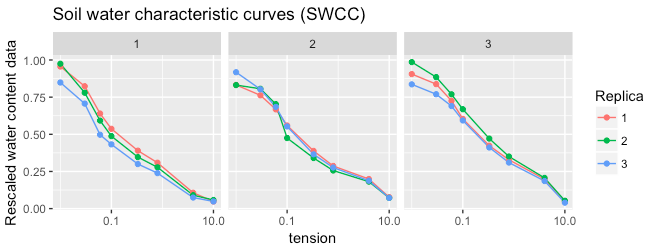
\includegraphics[width=16cm, height=5cm]{p1.png}
\end{figure}

\subsection*{Re-parameterization in terms of mean and precision}

First, a beta distribution parameterized in terms of shape parameters $\alpha$ and $\beta$ has as mean $\mu$ and variance $\sigma^2$:


$$\mu = \frac{\alpha}{\alpha+\beta}$$ 
$$\sigma^2 = \frac{\alpha \beta}{(\alpha+\beta)^2 (\alpha + \beta +1)}$$

Defining $\phi = \alpha + \beta$, we can write $\alpha = \phi \mu$ and $\beta = \phi (1-\mu)$. Now, the variance $\sigma^2$ can be written in terms of $\mu$ and $\phi$. With this re-parameterization, we can write that $y \sim B(\alpha, \beta)$ is equivalent to $y \sim B(\mu, \phi)$ with $E(y) = \mu$ and $Var(y) =\frac{\mu (1-\mu)}{\phi +1}$. As $\phi$ is the sum of two positive numbers, we have that $\phi > 0$ and that $\mu$ is in the interval (0,1). In his paper, \cite{cribari2009beta} justifies that $\phi$ can be seen as a precision parameter. This is because, for a fixed $\mu$, if we increases $\phi$, the variance of $y$ will decrease.

More discussion should be done about the parameter $\phi$. It is easier to assume that this parameter is constant for all the observations, but in general this is not true. In fact, as \cite{cribari2009beta} states, \textit{data in the interval [0,1] such as rates and proportions are usually heteroscedastic}. But, because of the objective of this project, a constant $\phi$ will be considered. Also, a consideration about the parameter $\mu$ should be made. The question about the parameter $\mu$, is: should we consider one parameter per observation ($\mu_{ijk}$) or is it better to consider $\mu_kj$ or $\mu_k$? (i for replica, j for depth soil and k for the levels of the regressors x). Different experiments will be done in this report. Assuming that $\phi$ is common for every observation (i.e. Homoscedasticity), we can write the basic model of the report as:

\begin{equation}
\tilde{y}_{kji}| \mu_{ijk}, \phi \sim B(\phi(\mu_{ijk}), \phi(1-\mu_{ijk}))
\end{equation}


\section{Priors for the parameters $\phi$ and $\mu_{ijk}$}

In this problem we do not have prior information for the apriori distribution, so uninformative prior distributions will be used. The restrictions of the problem states that $\beta_1, \beta_2$ and $\beta_3 > 0$. Then, as stated in \cite{costa2017bayesian}, \say{the parameters $\beta_1, \beta_2$ and $\beta_3$ have a broad interpretation of scale (possibly under a re-parameterization)}. Then, a prior gamma distribution with small shape and scale parameters can be used. On the other hand, the $\phi$ parameter can be considered as a precision parameter, then an uninformative gamma distribution with shape $\alpha = 0.01$ and rate $\beta = 0.01$ will be used.

\begin{figure}[ht!]
\centering
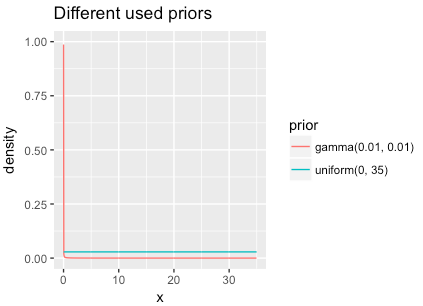
\includegraphics[width=9cm, height = 6cm]{p2.png}
\end{figure}


\subsection*{Including soil depth variability}
The first model is a pooled effects model. After this, to include the variability associated with the the soil depth, an independent effects and a hierarchical model will be tried. In the independent effects and hierarchical model, each $\beta_1, \beta_2$ and $\beta_3$ is a three dimensional vector, with one dimension for each soil depth. This way, in total nine $\beta$'s parameters will be estimated. In the case of the hierarchical model, the $\beta$'s associated at the same soil depth will have common uninformative hyperparameters (with distribution gamma(0.01, 0.01)). Finally, for the last two approaches, $\mu_kj$ will be considered (i.e. it will depend on the regressor value and on the soil depth). 

\subsection*{Number of iterations, chains, burning and thinning}
Stan is relatively faster that Bugs. For this reason, more iterations can be done in the same time. In this report, two chains were computed with 150,000 iterations each one. To reduce the autocorrelation, a thinning of 10 was done. Also, by default Stan takes a burning of the 50\% of the iterations, so at the end 7,500 iterations were taken into account.

\subsection*{Convergence and autocorrelation}

The Stan default output shows the $\widehat{R}$ statistic. As stated in the documentation, we should be careful of values larger than 1.1 of smaller than .9. Also, they suggest to make an histogram of the $\widehat{R}$ statistics, to see if some parameter of the model has convergence problems. The autocorrelation plots also were analyzed (The convergence and autocorrelation plots are in the appendix section).

\newpage

%%%%%%%%%%%%%%%%%%%%%%%%%%%%%%%%%%%%%%%%%%%%%%%%%%%%%%%%%%%%%%%%%%%%%%%%%%%%%%%%%%%%%%%%%%%%
%%%%%%%%%%%%%%%%%%%%%%%%%%%%%%%%%%%%%%%%%%%%%%%%%%%%%%%%%%%%%%%%%%%%%%%%%%%%%%%%%%%%%%%%%%%%
%%%%%%%%%%%%%%%%%%%%%%%%%%%%%%%%%%%%%%%%%%%%%%%%%%%%%%%%%%%%%%%%%%%%%%%%%%%%%%%%%%%%%%%%%%%%
%%%%%%%%%%%%%%%%%%%%%%%%%%%%%%%%%%%%%%%%%%%%%%%%%%%%%%%%%%%%%%%%%%%%%%%%%%%%%%%%%%%%%%%%%%%%
\section{Pooled effects for the soil depth variability}
For the first model, $\mu$ will consider the effect of the values in the regressor $x$ (i.e. will use the parameter $\mu_k$, with $k = 1,..., 8$), with $\mu_k = \frac{1}{1+(\beta_1 x_k)^{\beta_2}}$ and each $\beta_1, \beta_2$ distributed $Gamma(0.01, 0.01)$ for the Gardner’s expression. And with $\mu_k = \frac{1}{[1+(\beta_1 x_k)^{\beta_2}]^{\beta_3}}$ with $\beta_1, \beta_2, \beta_3$ distributed $Gamma(0.01, 0.01)$ for the van Genuchten expression.

\subsection*{Gardner's model}
\subsubsection*{\underline{Fitted Values}}

\begin{minipage}{0.50\textwidth}
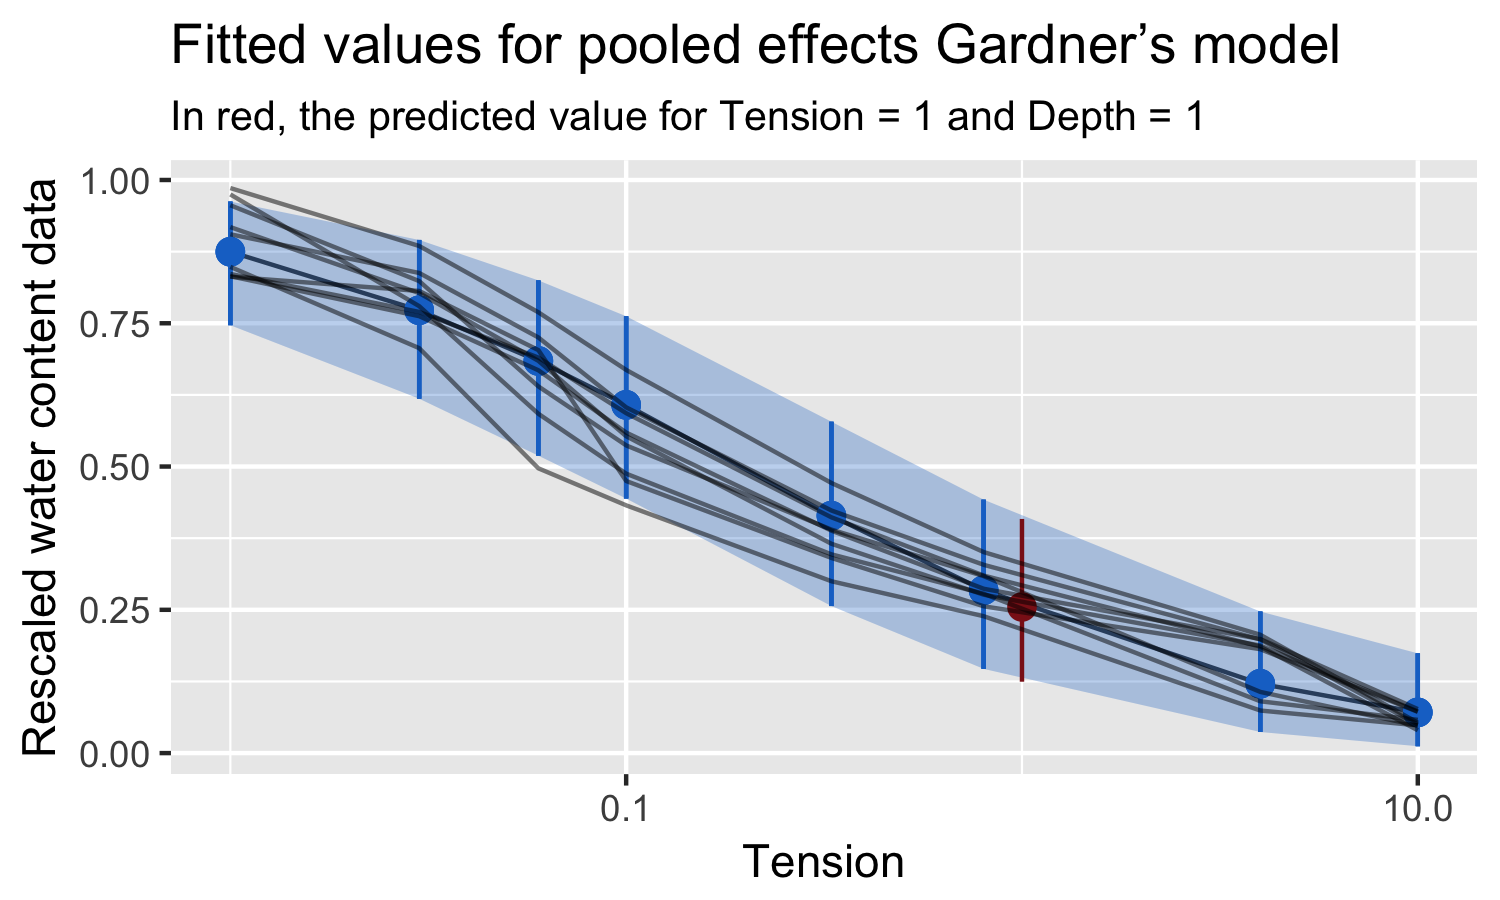
\includegraphics[width=\linewidth]{pooled_2pars_pred.png}
\end{minipage}
\begin{minipage}{0.50\textwidth}
The fitted values are shown in the left graph. As this model does not considers the depth levels, the plot just shows the model at different levels of the regressor $x$ (Tension level). The blue points are the mean value of the model given regressor $x$ (with a 95\% credible interval). The gray lines show the different replicas taken at the depth levels. Finally, the red line and point, represent the predictive distribution given the regresor $x=1$.
\end{minipage}

\subsubsection*{\underline{Convergence and autocorrelation}}
\begin{minipage}{0.50\textwidth}
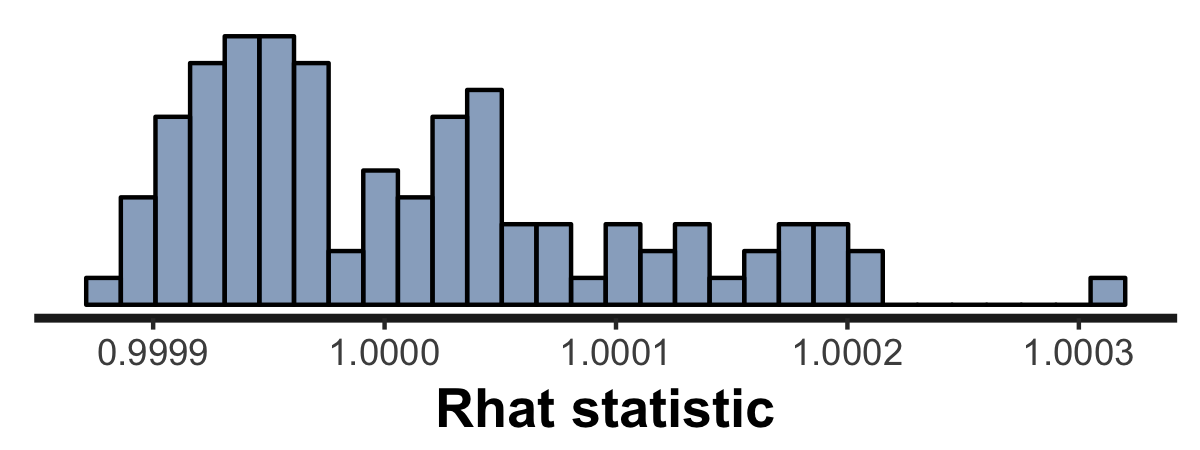
\includegraphics[width=\linewidth]{pooled_2pars_rhat.png}
\end{minipage}
\begin{minipage}{0.50\textwidth}
Here is the histogram of the $\widehat{R}$ statistic. All values are close to 1: no problem of convergence. In addition, the autocorrelation plots in the Appendix A does not show any problem.
\end{minipage}


\subsubsection*{\underline{Posterior summaries}}
The below graph show the posterior distribution density for the parameters $\beta_1$, $\beta_2$, $\phi$ and $y_{pred}$. In addition, the posterior summaries are given.

\begin{figure}[ht!]
\centering
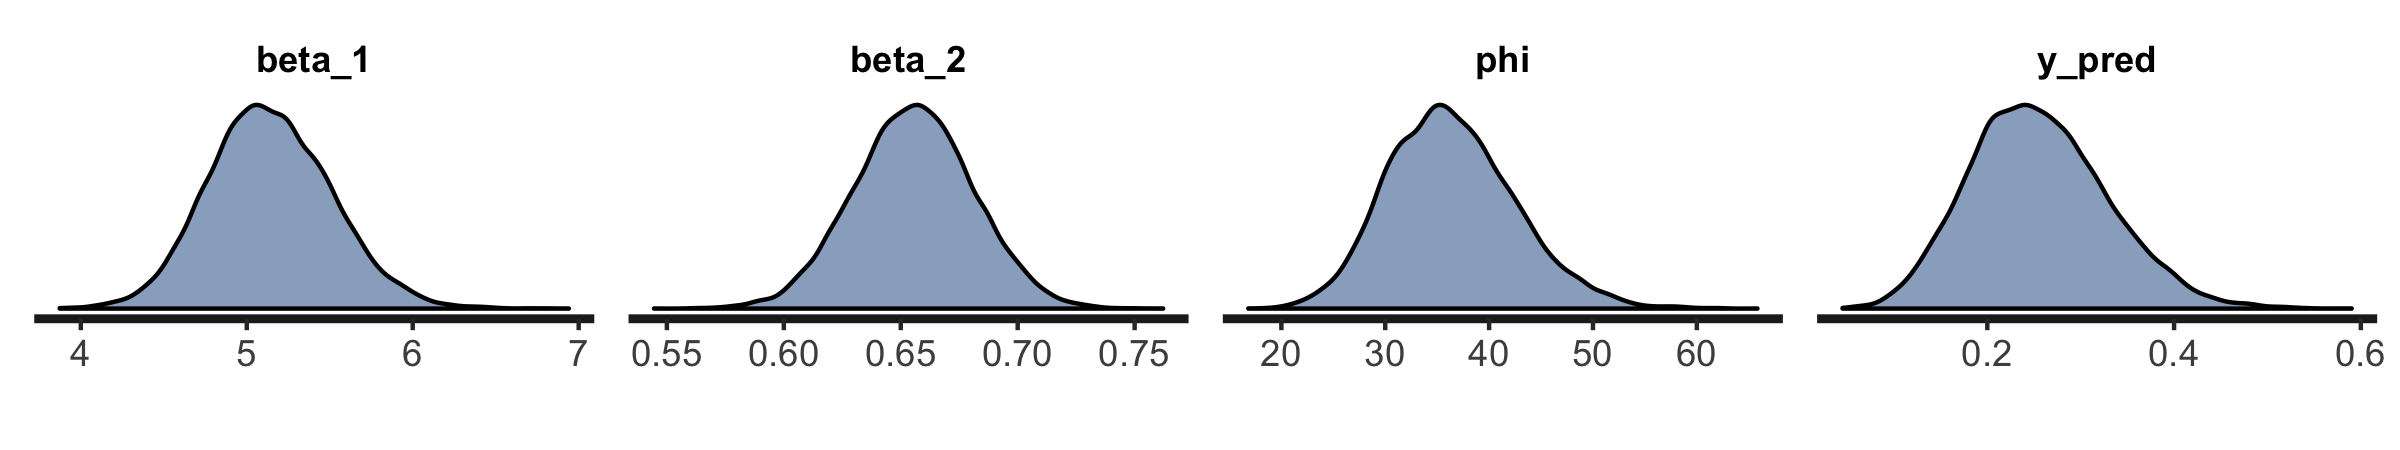
\includegraphics[width=13cm]{pooled_2pars_dens.png}
\end{figure}

\begin{figure}[ht!]
\centering
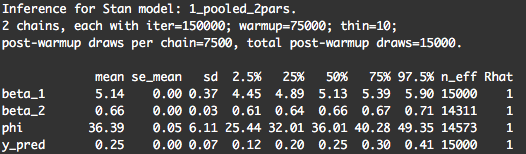
\includegraphics[width=9cm]{p01.png}
\end{figure}

 \newpage
 \subsection*{\underline{van Genuchten model}}

\subsubsection*{\underline{Fitted Values}}
\begin{minipage}{0.50\textwidth}
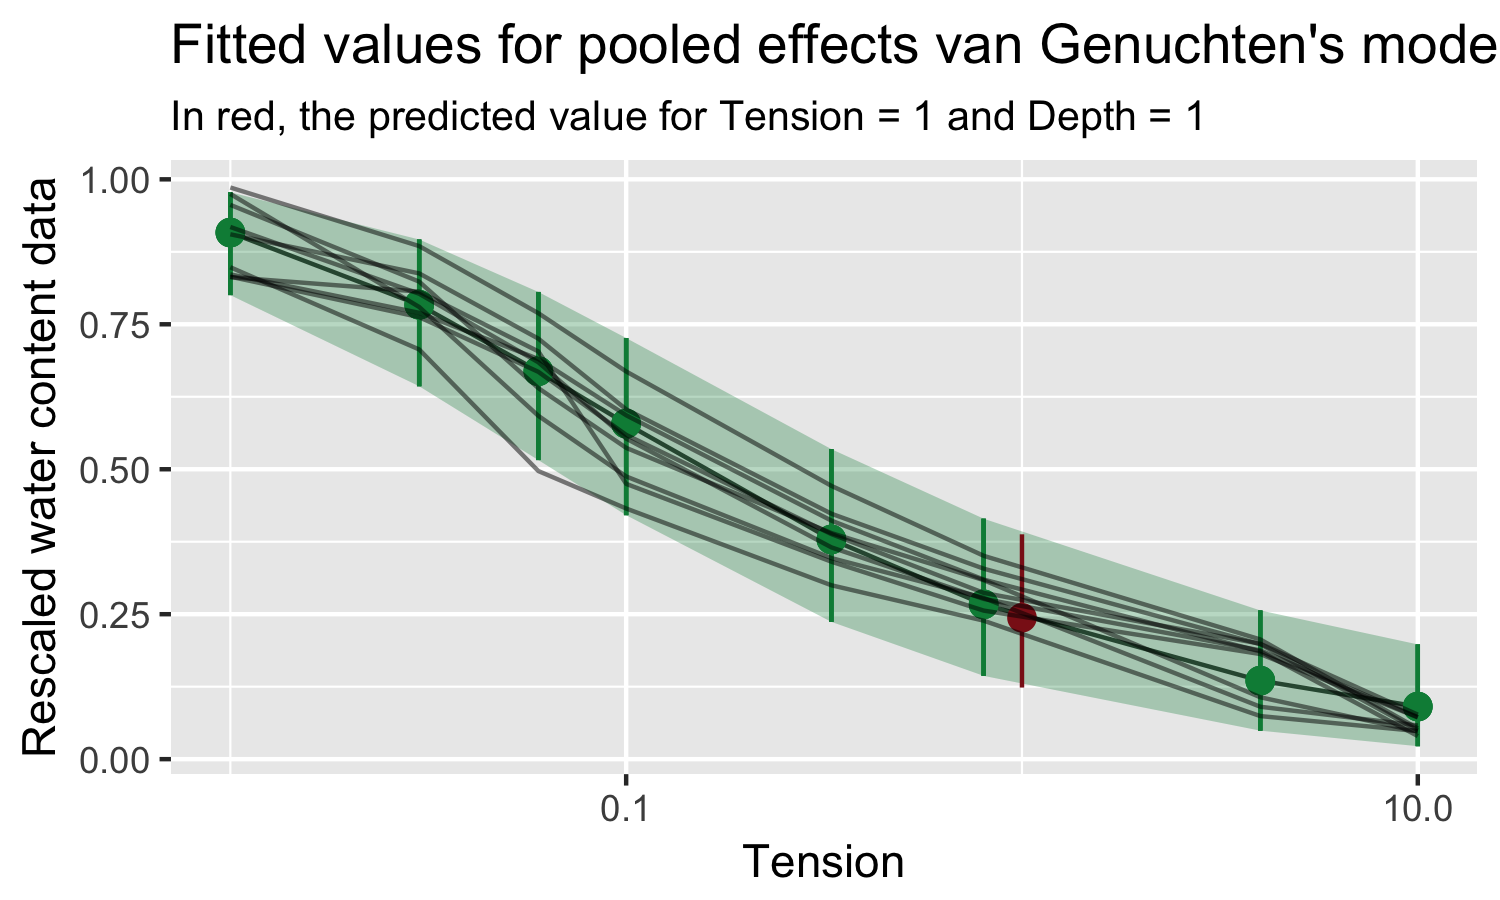
\includegraphics[width=\linewidth]{pooled_3pars_pred.png}
\end{minipage}
\begin{minipage}{0.50\textwidth}
The fitted values are shown in the left graph. As this model does not considers the depth levels, the plot just shows the model at different levels of the regressor $x$ (Tension level). The green points are the mean value of the model given regressor $x$ (with a 95\% credible interval). The gray lines show the different replicas taken at the depth levels. Finally, the red line and point, represent the predictive distribution given the regresor $x$.
\end{minipage}


\subsubsection*{\underline{Convergence and autocorrelation}}
\begin{minipage}{0.50\textwidth}
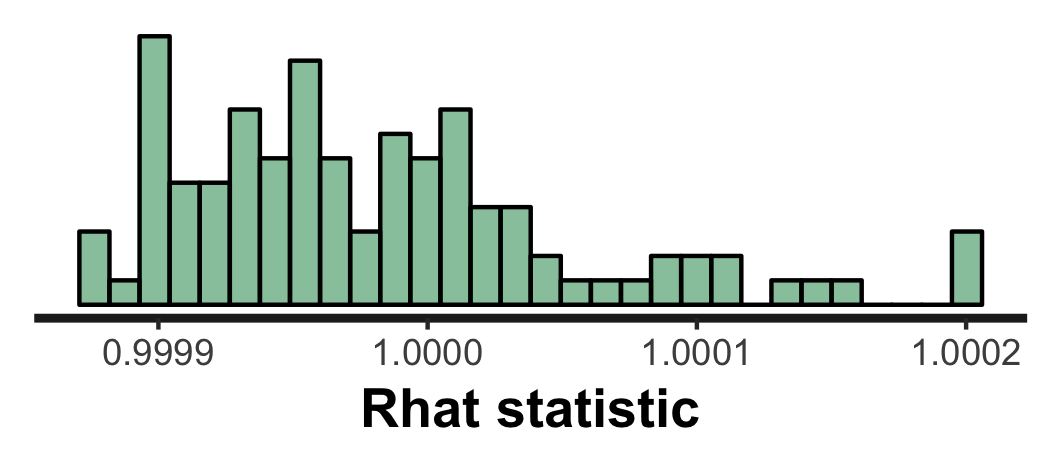
\includegraphics[width=\linewidth]{pooled_3pars_rhat.png}
\end{minipage}
\begin{minipage}{0.50\textwidth}
Here is the histogram of the $\widehat{R}$ statistic. All values are close to 1: no problem of convergence. In addition, the autocorrelation plots in the Appendix A does not show any problem.
\end{minipage}

\subsubsection*{\underline{Posterior summaries}}
The below graph show the posterior distribution density for the parameters $\beta_1$, $\beta_2$, $\beta_3$ $\phi$ and $y_{pred}$. In addition, the posterior summaries are given.
\begin{figure}[ht!]
\centering
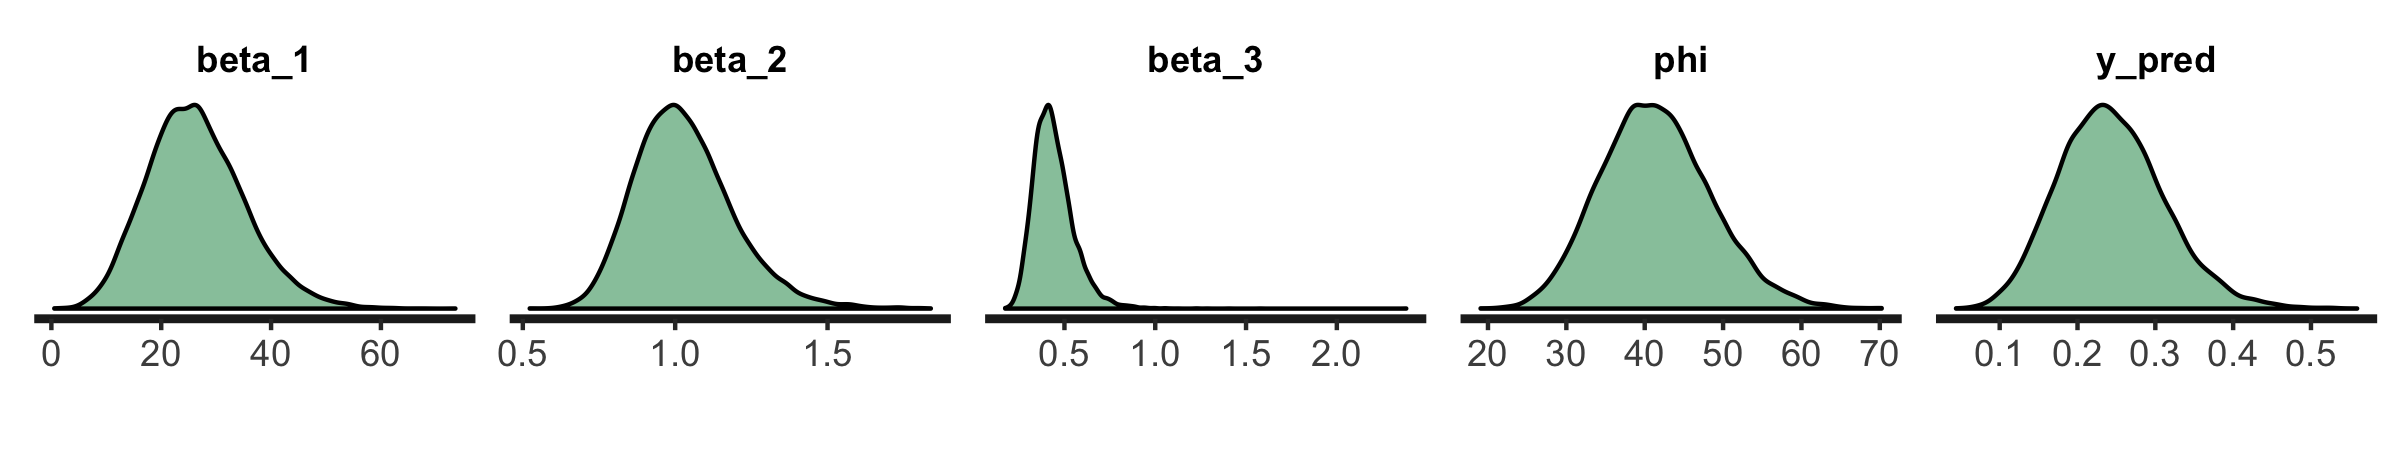
\includegraphics[width=16cm]{pooled_3pars_dens.png}
\end{figure}

\begin{figure}[ht!]
\centering
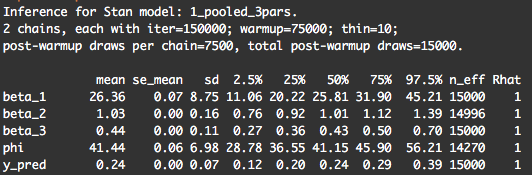
\includegraphics[width=10cm]{p02.png}
\end{figure}


%%%%%%%%%%%%%%%%%%%%%%%%%%%%%%%%%%%%%%%%%%%%%%%%%%%%%%%%%%%%%%%%%%%%%%%%%%%%%%%%%%%%%%%%%%%%
%%%%%%%%%%%%%%%%%%%%%%%%%%%%%%%%%%%%%%%%%%%%%%%%%%%%%%%%%%%%%%%%%%%%%%%%%%%%%%%%%%%%%%%%%%%%
%%%%%%%%%%%%%%%%%%%%%%%%%%%%%%%%%%%%%%%%%%%%%%%%%%%%%%%%%%%%%%%%%%%%%%%%%%%%%%%%%%%%%%%%%%%%
%%%%%%%%%%%%%%%%%%%%%%%%%%%%%%%%%%%%%%%%%%%%%%%%%%%%%%%%%%%%%%%%%%%%%%%%%%%%%%%%%%%%%%%%%%%%

\newpage
\section{Independent effects for the soil depth variability}
For this second model, $\mu$ will just consider the effect of the values of the regressor $x$ and the effect of soil depth as a hierarchical effect (i.e. $\mu_{kj}$, with $k = 1,..., 8$ and $j = 1,2,3$), with $\mu_{kj} = \frac{1}{1+(\beta_{1j} x_k)^{\beta_{2j}}}$ and each $\beta_{1j}, \beta_{2j}$ distributed $Gamma(0.01, 0.01)$ for $j = 1,2,3$ for the Gardner’s expression. And with $\mu_{kj} = \frac{1}{[1+(\beta_{1j} x_k)^{\beta_{2j}}]^{\beta_{3j}}}$ for $j = 1,2,3$ and each $\beta_{1j}, \beta_{2j}, \beta_{3j}$ distributed $Gamma(0.01, 0.01)$ for $j = 1,2,3$ for the van Genuchten expression.

\subsection*{\underline{Gardner's model}}
\subsubsection*{\underline{Fitted Values}}

The fitted values are shown in the below graph. Now, the model considers the depth levels and there is one plot for each one. The blue points are the mean value of the model given regressor $x$ (with a 95\% credible interval). The gray lines show the different replicas taken at the depth levels. Finally, the red line and point, represent the predictive distribution given the regresor $x = 1, depth = 1$.

\begin{figure}[ht!]
\centering
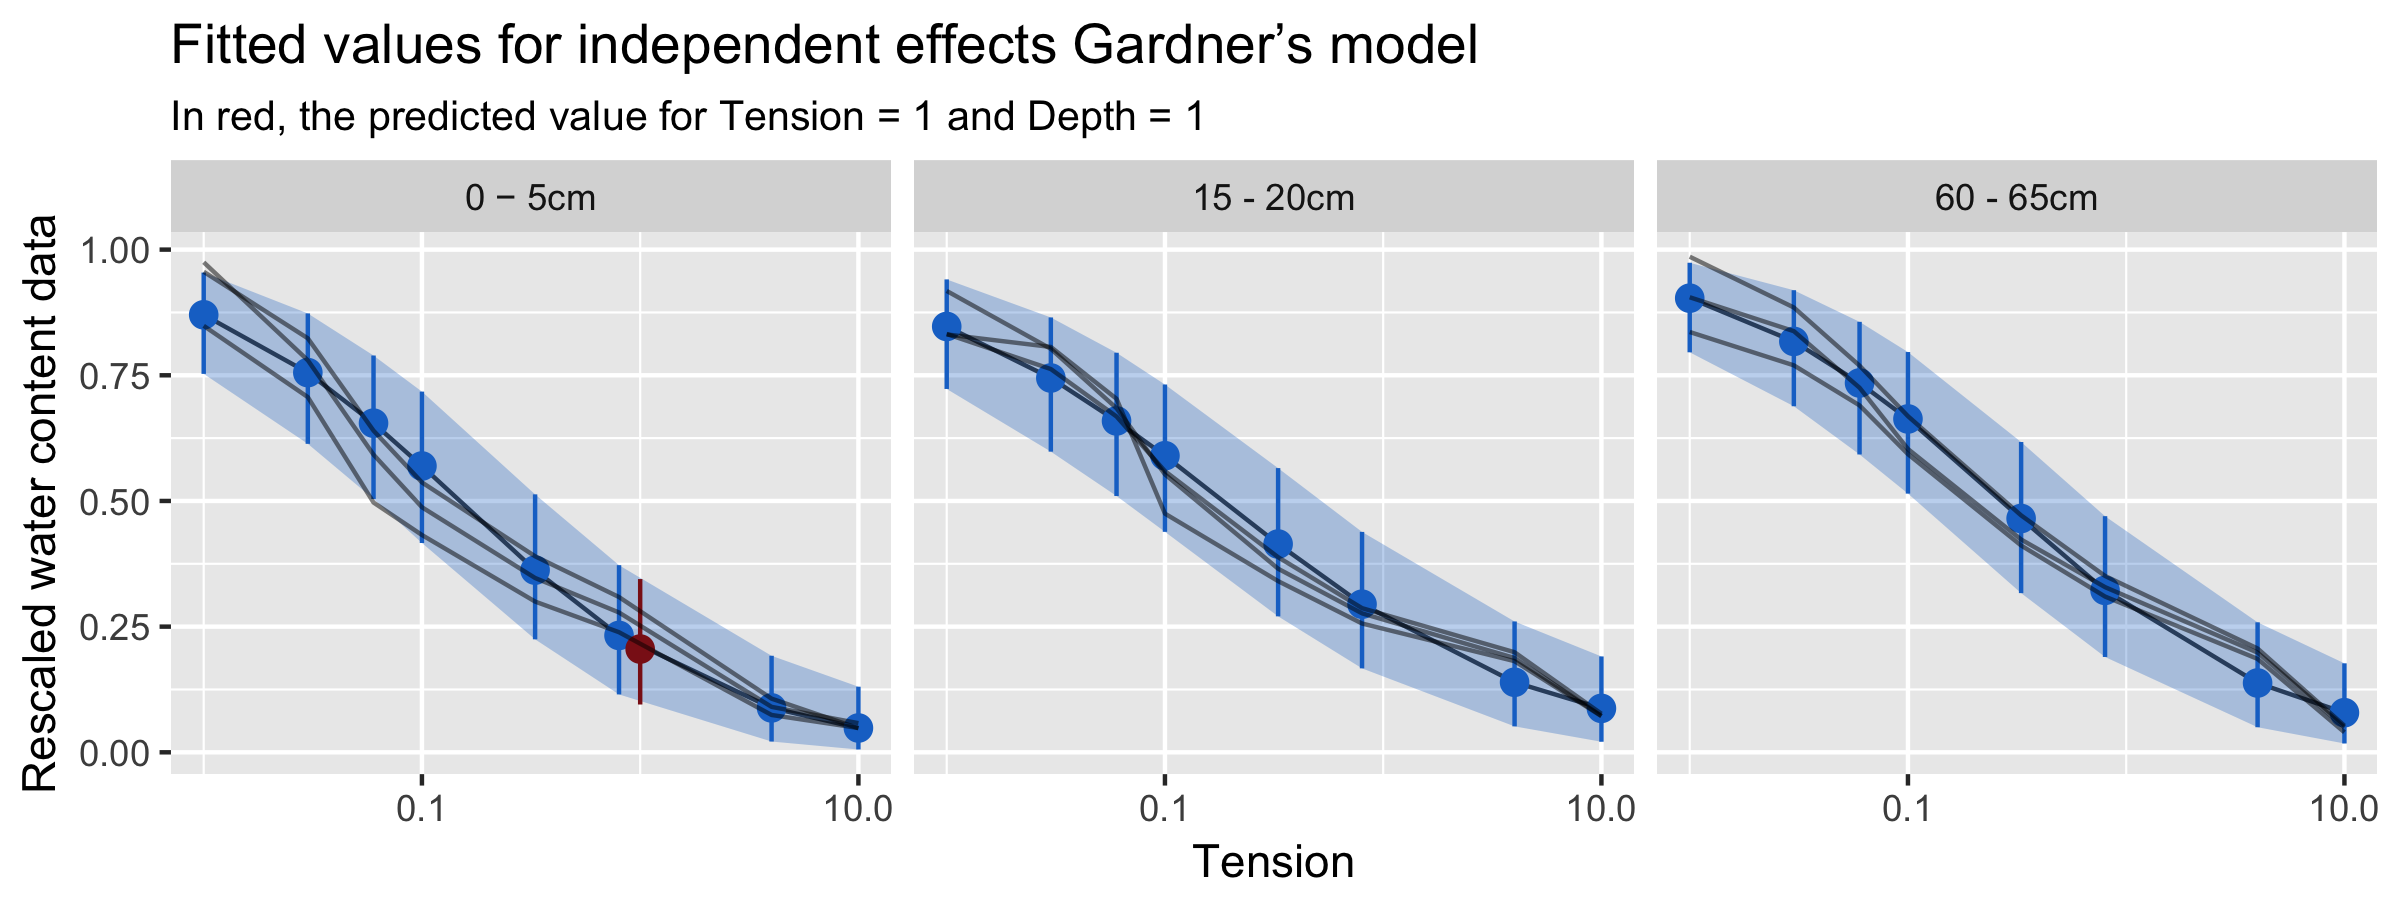
\includegraphics[width=14cm]{indep_2pars_pred.png}
\end{figure}

\subsubsection*{\underline{Convergence and autocorrelation}}
\begin{minipage}{0.50\textwidth}
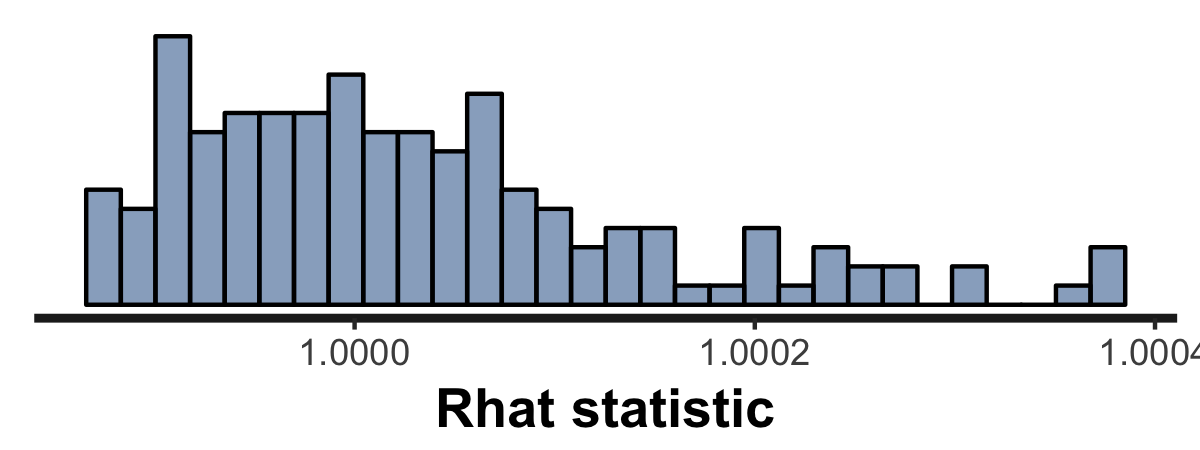
\includegraphics[width=\linewidth, height = 2.5cm]{indep_2pars_rhat.png}
\end{minipage}
\begin{minipage}{0.50\textwidth}
Here is the histogram of the $\widehat{R}$ statistic. All values are close to 1: no problem of convergence. In addition, the autocorrelation plots in the Appendix A does not show any problem.
\end{minipage}

\subsubsection*{\underline{Posterior summaries}}
The below graph show the posterior distribution density for the parameters $\beta_1$, $\beta_2$, $\phi$ and $y_{pred}$. In addition, the posterior summaries are given. As can be seen, now there is one estimate of $\beta_1,\beta_2,\beta_3$ per depth.
\begin{minipage}{0.50\textwidth}
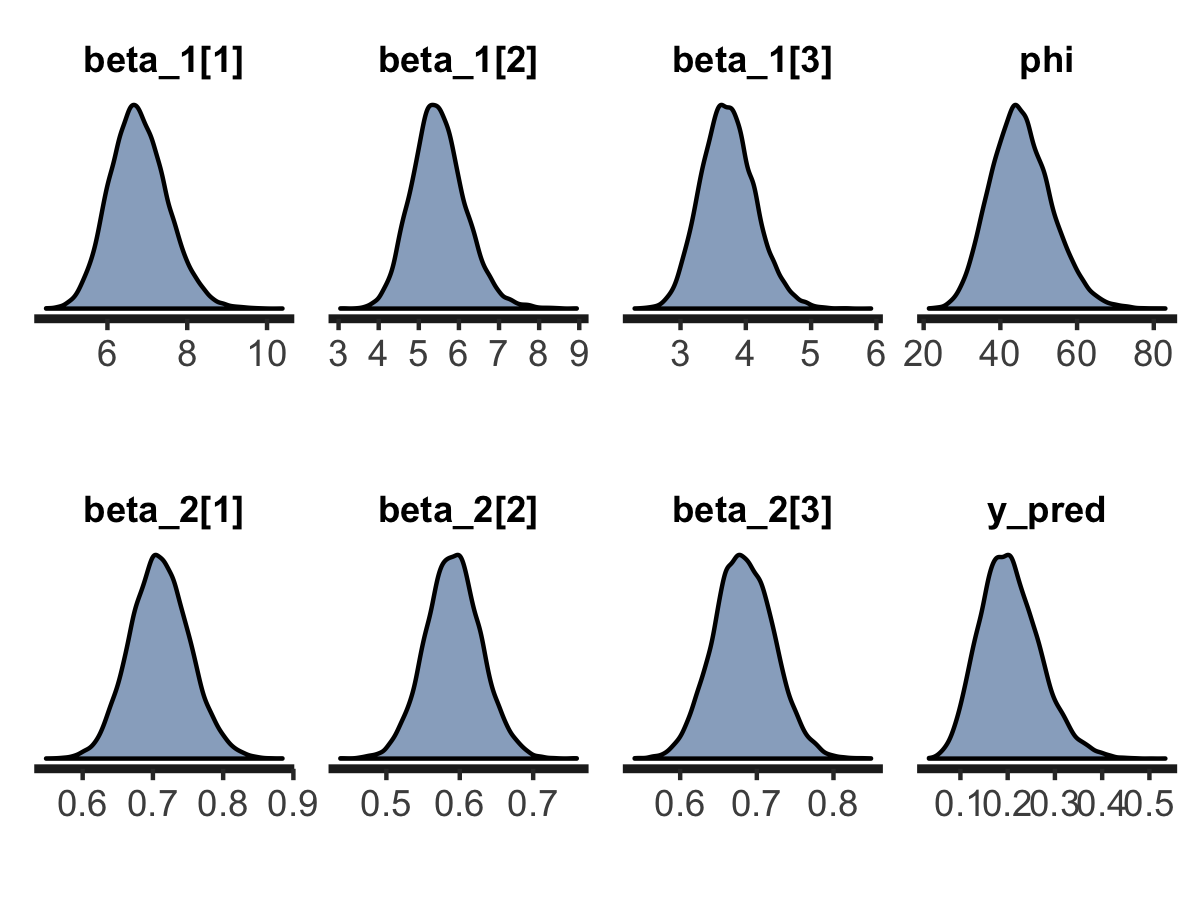
\includegraphics[width=\linewidth, height = 4.5cm]{indep_2pars_dens.png}
\end{minipage}
\begin{minipage}{0.50\textwidth}
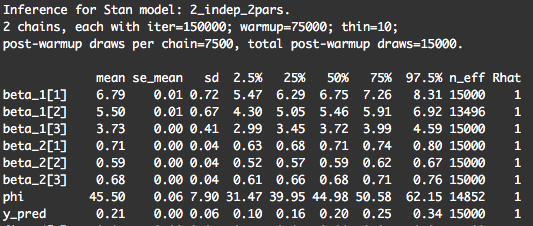
\includegraphics[width=\linewidth, height = 4.5cm]{p03.png}
\end{minipage}


\newpage


\subsection*{\underline{van Genuchten model}}
\subsubsection*{\underline{Fitted Values}}

The fitted values are shown in the below graph. Now, the model considers the depth levels and there is one plot for each one. The green points are the mean value of the model given regressor $x$ (with a 95\% credible interval). The gray lines show the different replicas taken at the depth levels. Finally, the red line and point, represent the predictive distribution given the regresor $x = 1, depth = 1$.\begin{figure}[ht!]
\centering
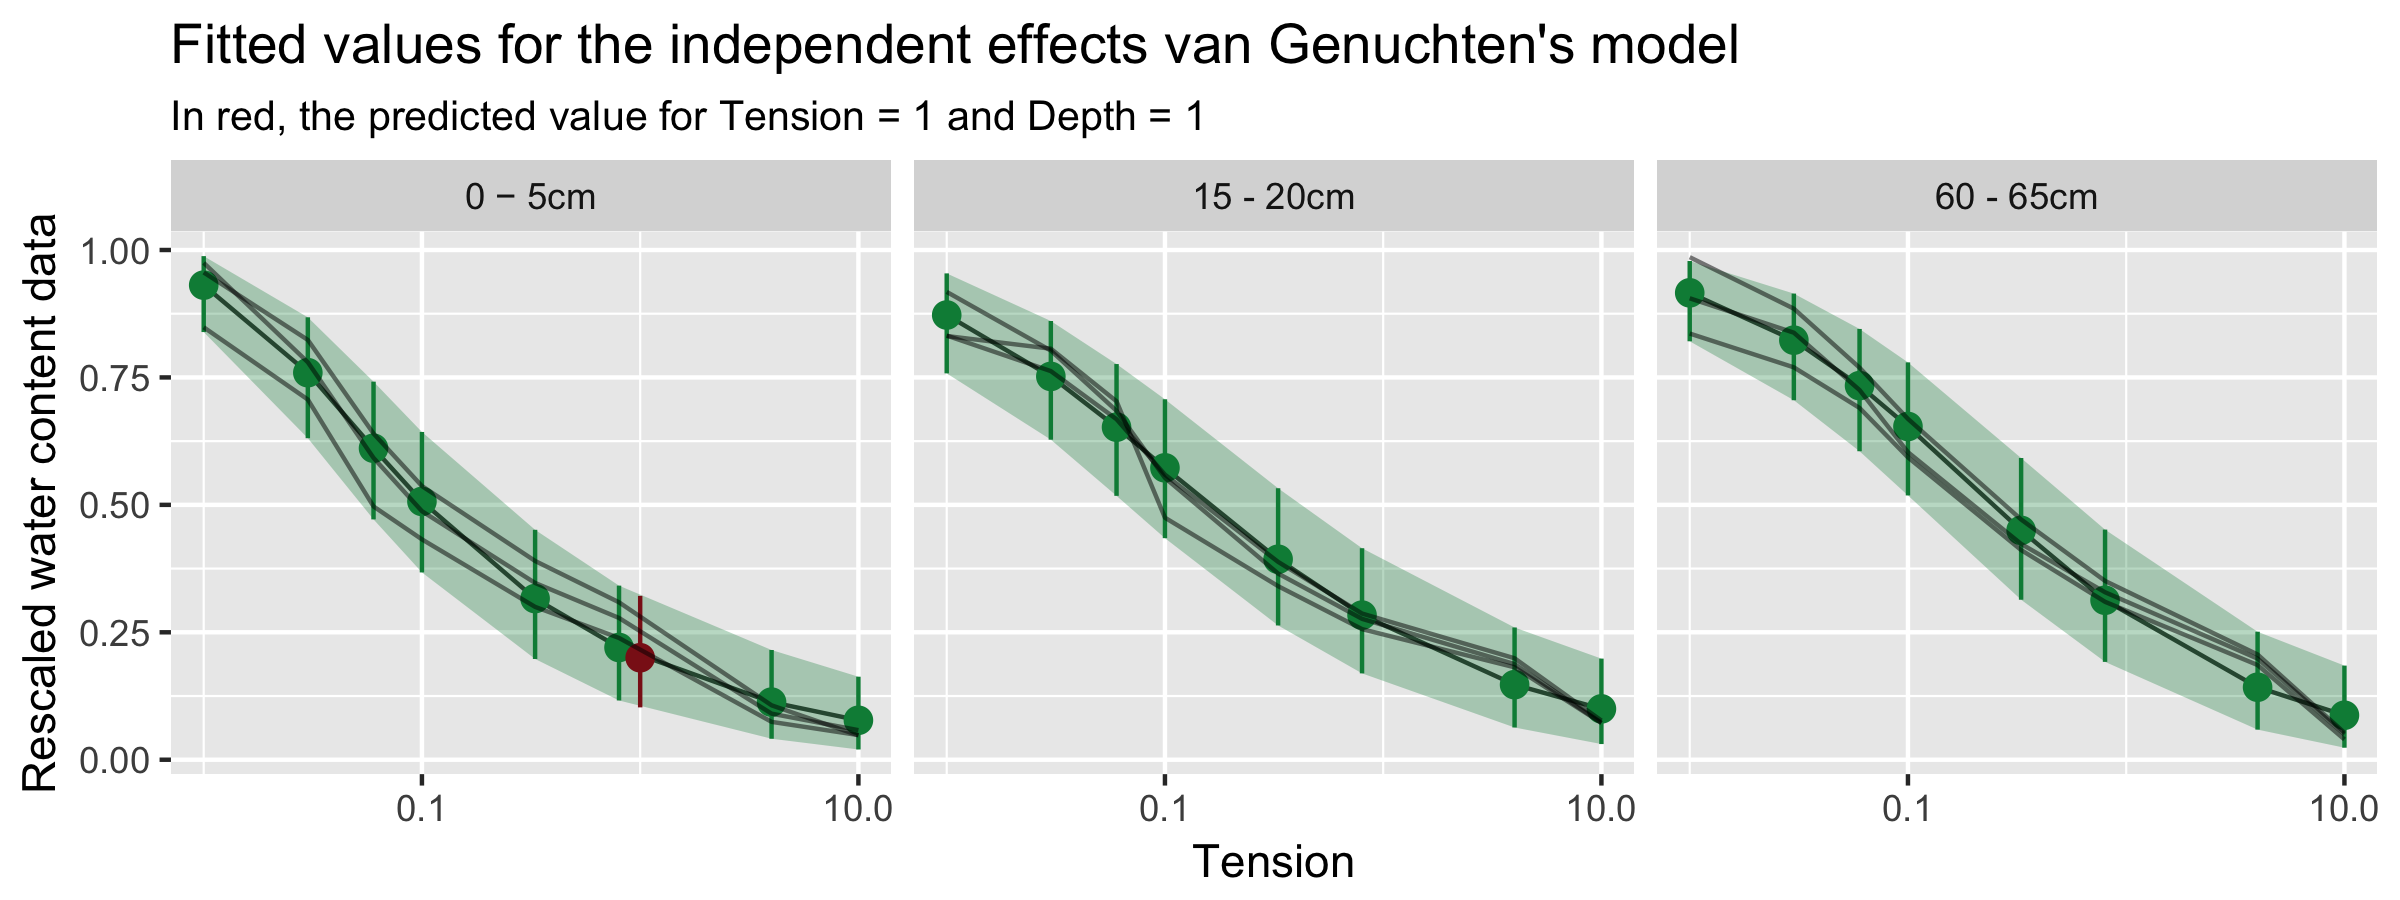
\includegraphics[width=16cm]{indep_3pars_pred.png}
\end{figure}

\subsubsection*{\underline{Convergence and autocorrelation}}
\begin{minipage}{0.50\textwidth}
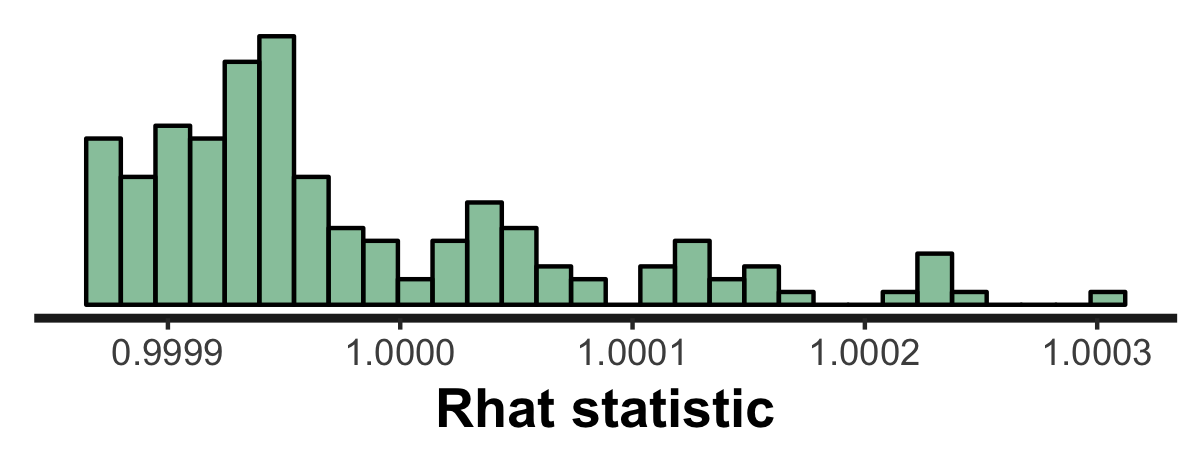
\includegraphics[width=\linewidth]{indep_3pars_rhat.png}
\end{minipage}
\begin{minipage}{0.50\textwidth}
Here is the histogram of the $\widehat{R}$ statistic. All values are close to 1: no problem of convergence. In addition, the autocorrelation plots in the Appendix A does not show any problem.
\end{minipage}

\subsubsection*{\underline{Posterior summaries}}
The below graph show the posterior distribution density for the parameters $\beta_1$, $\beta_2$, $\beta_3$ $\phi$ and $y_{pred}$. In addition, the posterior summaries are given. As can be seen, now there is one estimate of $\beta_1,\beta_2,\beta_3$ per depth.

\begin{minipage}{0.50\textwidth}
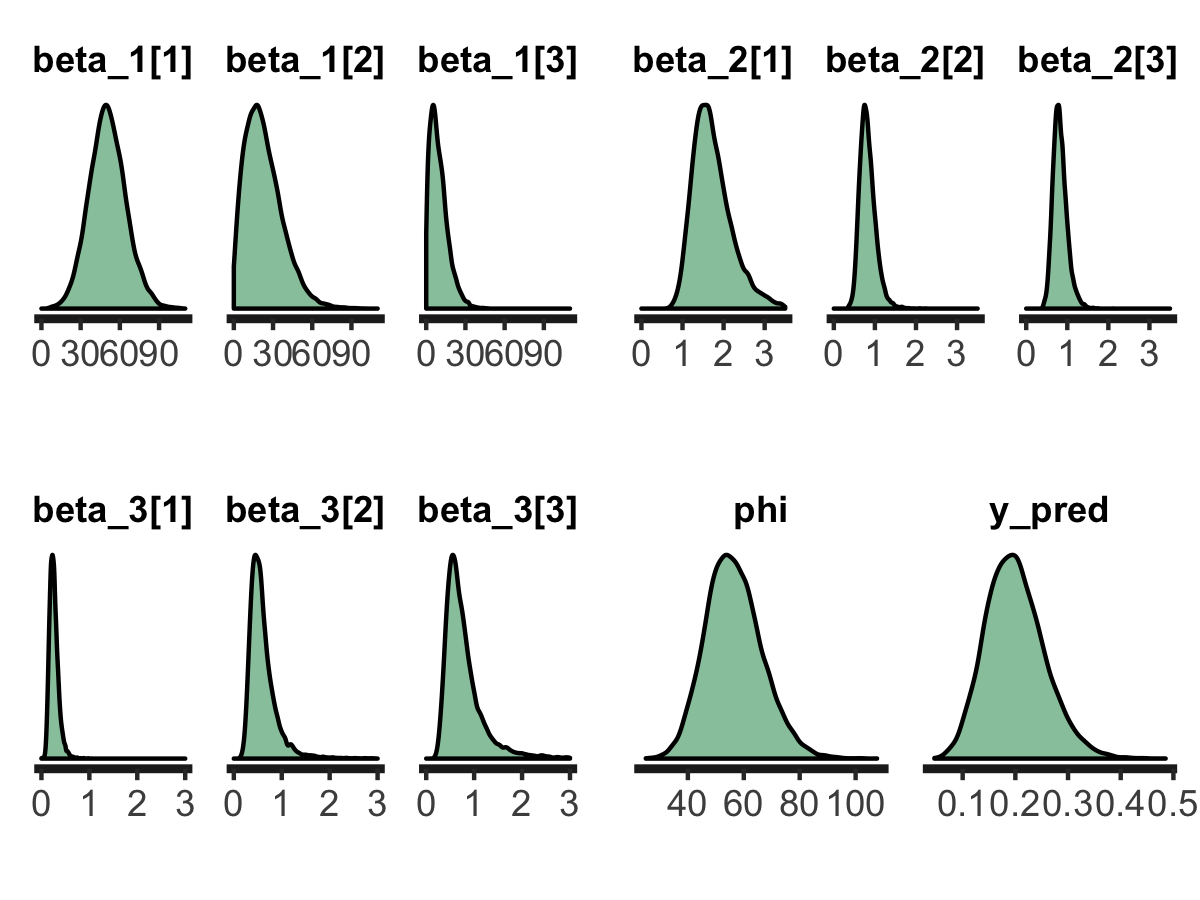
\includegraphics[width=\linewidth,]{indep_3pars_dens.png}
\end{minipage}
\begin{minipage}{0.50\textwidth}
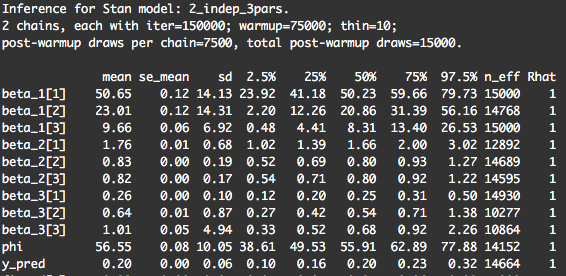
\includegraphics[width=\linewidth]{p04.png}
\end{minipage}

% %%%%%%%%%%%%%%%%%%%%%%%%%%%%%%%%%%%%%%%%%%%%%%%%%%%%%%%%%%%%%%%%%%%%%%%%%%%%%%%%%%%%%%%%%%%%
% %%%%%%%%%%%%%%%%%%%%%%%%%%%%%%%%%%%%%%%%%%%%%%%%%%%%%%%%%%%%%%%%%%%%%%%%%%%%%%%%%%%%%%%%%%%%
% %%%%%%%%%%%%%%%%%%%%%%%%%%%%%%%%%%%%%%%%%%%%%%%%%%%%%%%%%%%%%%%%%%%%%%%%%%%%%%%%%%%%%%%%%%%%
% %%%%%%%%%%%%%%%%%%%%%%%%%%%%%%%%%%%%%%%%%%%%%%%%%%%%%%%%%%%%%%%%%%%%%%%%%%%%%%%%%%%%%%%%%%%%
\newpage
\section{Hierarchical modelling to include soil depth variability}
For the third model, $\mu$ will just consider the effect of the values of the regressor $x$ and the effect of soil depth variability as an independent effect (i.e. $\mu_{kj}$, with $k = 1,..., 8$ and $j = 1,2,3$), with $\mu_{kj} = \frac{1}{1+(\beta_{1j} x_k)^{\beta_{2j}}}$ and each $\beta_{1j}, \beta_{2j}$ distributed $Gamma(0.01, 0.01)$  for $j = 1,2,3$ for the Gardner’s expression. And with $\mu_{kj} = \frac{1}{[1+(\beta_{1j} x_k)^{\beta_{2j}}]^{\beta_{3j}}}$ for $j = 1,2,3$ each $\beta_{1j}, \beta_{2j}, \beta_{3j}$ distributed $Gamma(0.01, 0.01)$ for $j = 1,2,3$ for the van Genuchten expression.

\subsection*{\underline{Gardner's model}}
\subsubsection*{\underline{Fitted Values}}

The fitted values are shown in the below graph. Now, the model considers the depth levels and there is one plot for each one. The blue points are the mean value of the model given regressor $x$ (with a 95\% credible interval). The gray lines show the different replicas taken at the depth levels. Finally, the red line and point, represent the predictive distribution given the regresor $x = 1, depth = 1$.
\begin{figure}[ht!]
\centering
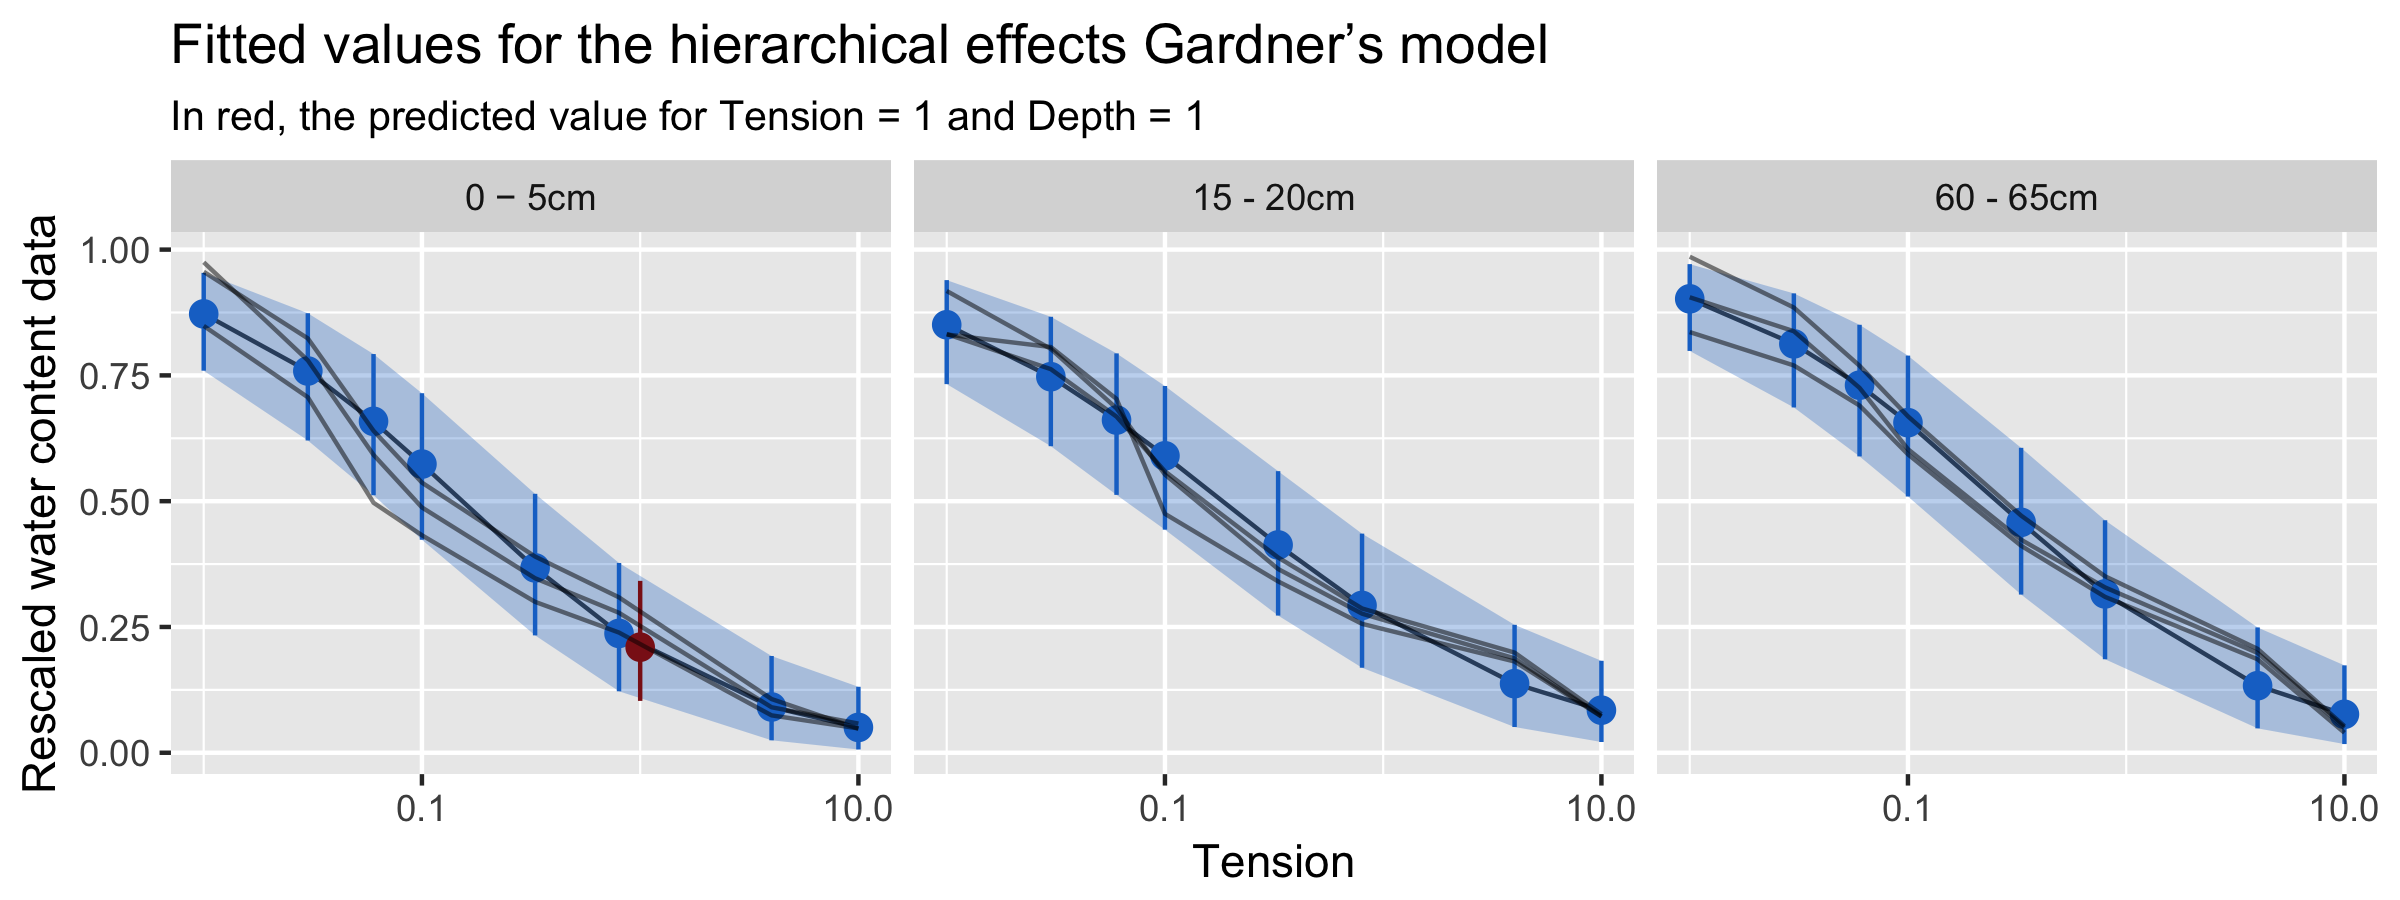
\includegraphics[width=14cm]{hier_2pars_pred.png}
\end{figure}

\subsubsection*{\underline{Convergence and autocorrelation}}
\begin{minipage}{0.50\textwidth}
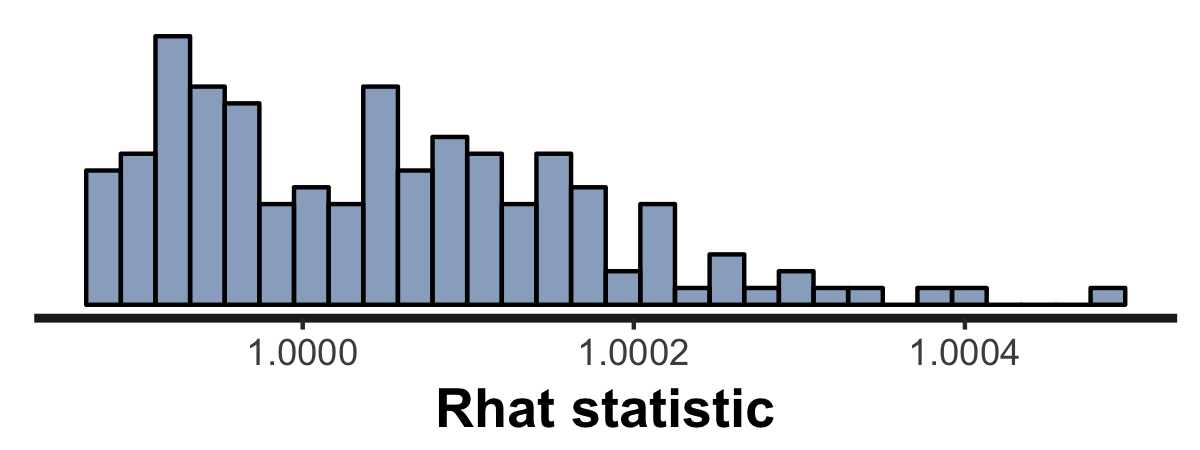
\includegraphics[width=\linewidth, height = 2.5cm]{hier_2pars_rhat.png}
\end{minipage}
\begin{minipage}{0.50\textwidth}
Here is the histogram of the $\widehat{R}$ statistic. All values are close to 1: no problem of convergence. In addition, the autocorrelation plots in the Appendix A does not show any problem.
\end{minipage}


\subsubsection*{\underline{Posterior summaries}}
The below graph show the posterior distribution density for the parameters $\beta_1$, $\beta_2$, $\phi$ and $y_{pred}$. In addition, the posterior summaries are given. As can be seen, now there is one estimate of $\beta_1,\beta_2$ per depth. Also, the hyperparameters estimates for each $beta_1, beta_2$ are shown (alpha1, alpha2, beta1,beta2).
\begin{minipage}{0.50\textwidth}
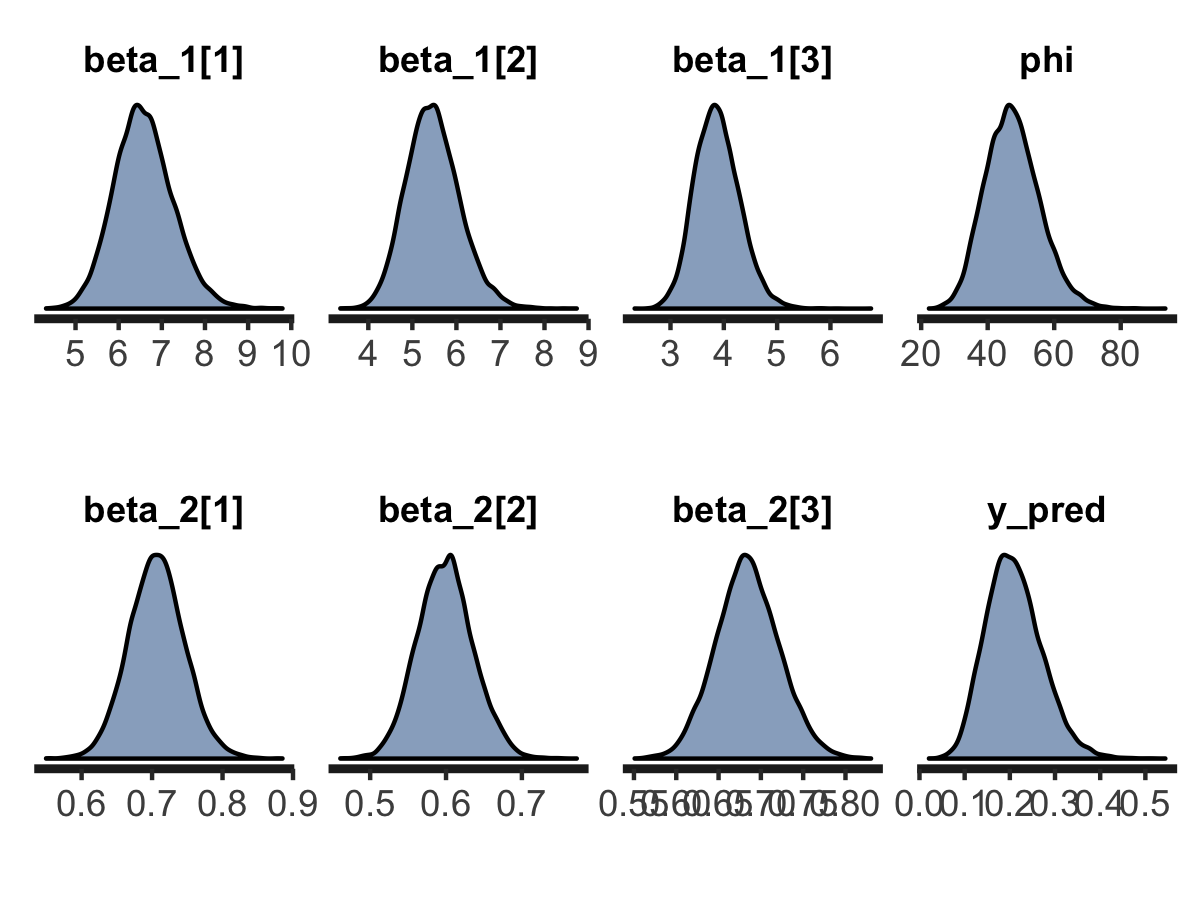
\includegraphics[width=\linewidth,height = 4cm]{hier_2pars_dens.png}
\end{minipage}
\begin{minipage}{0.50\textwidth}
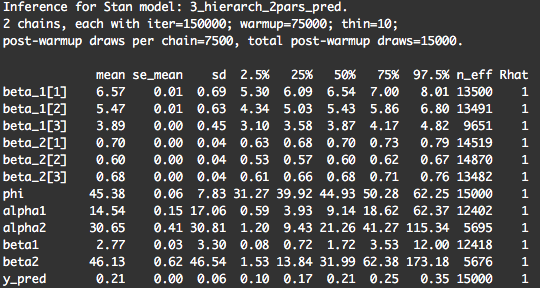
\includegraphics[width=\linewidth,height = 4cm]{p05.png}
\end{minipage}


\newpage


\subsection*{\underline{van Genuchten model}}
\subsubsection*{\underline{Fitted Values}}

The fitted values are shown in the below graph. Now, the model considers the depth levels and there is one plot for each one. The green points are the mean value of the model given regressor $x$ (with a 95\% credible interval). The gray lines show the different replicas taken at the depth levels. Finally, the red line and point, represent the predictive distribution given the regresor $x = 1, depth = 1$.

\begin{figure}[ht!]
\centering
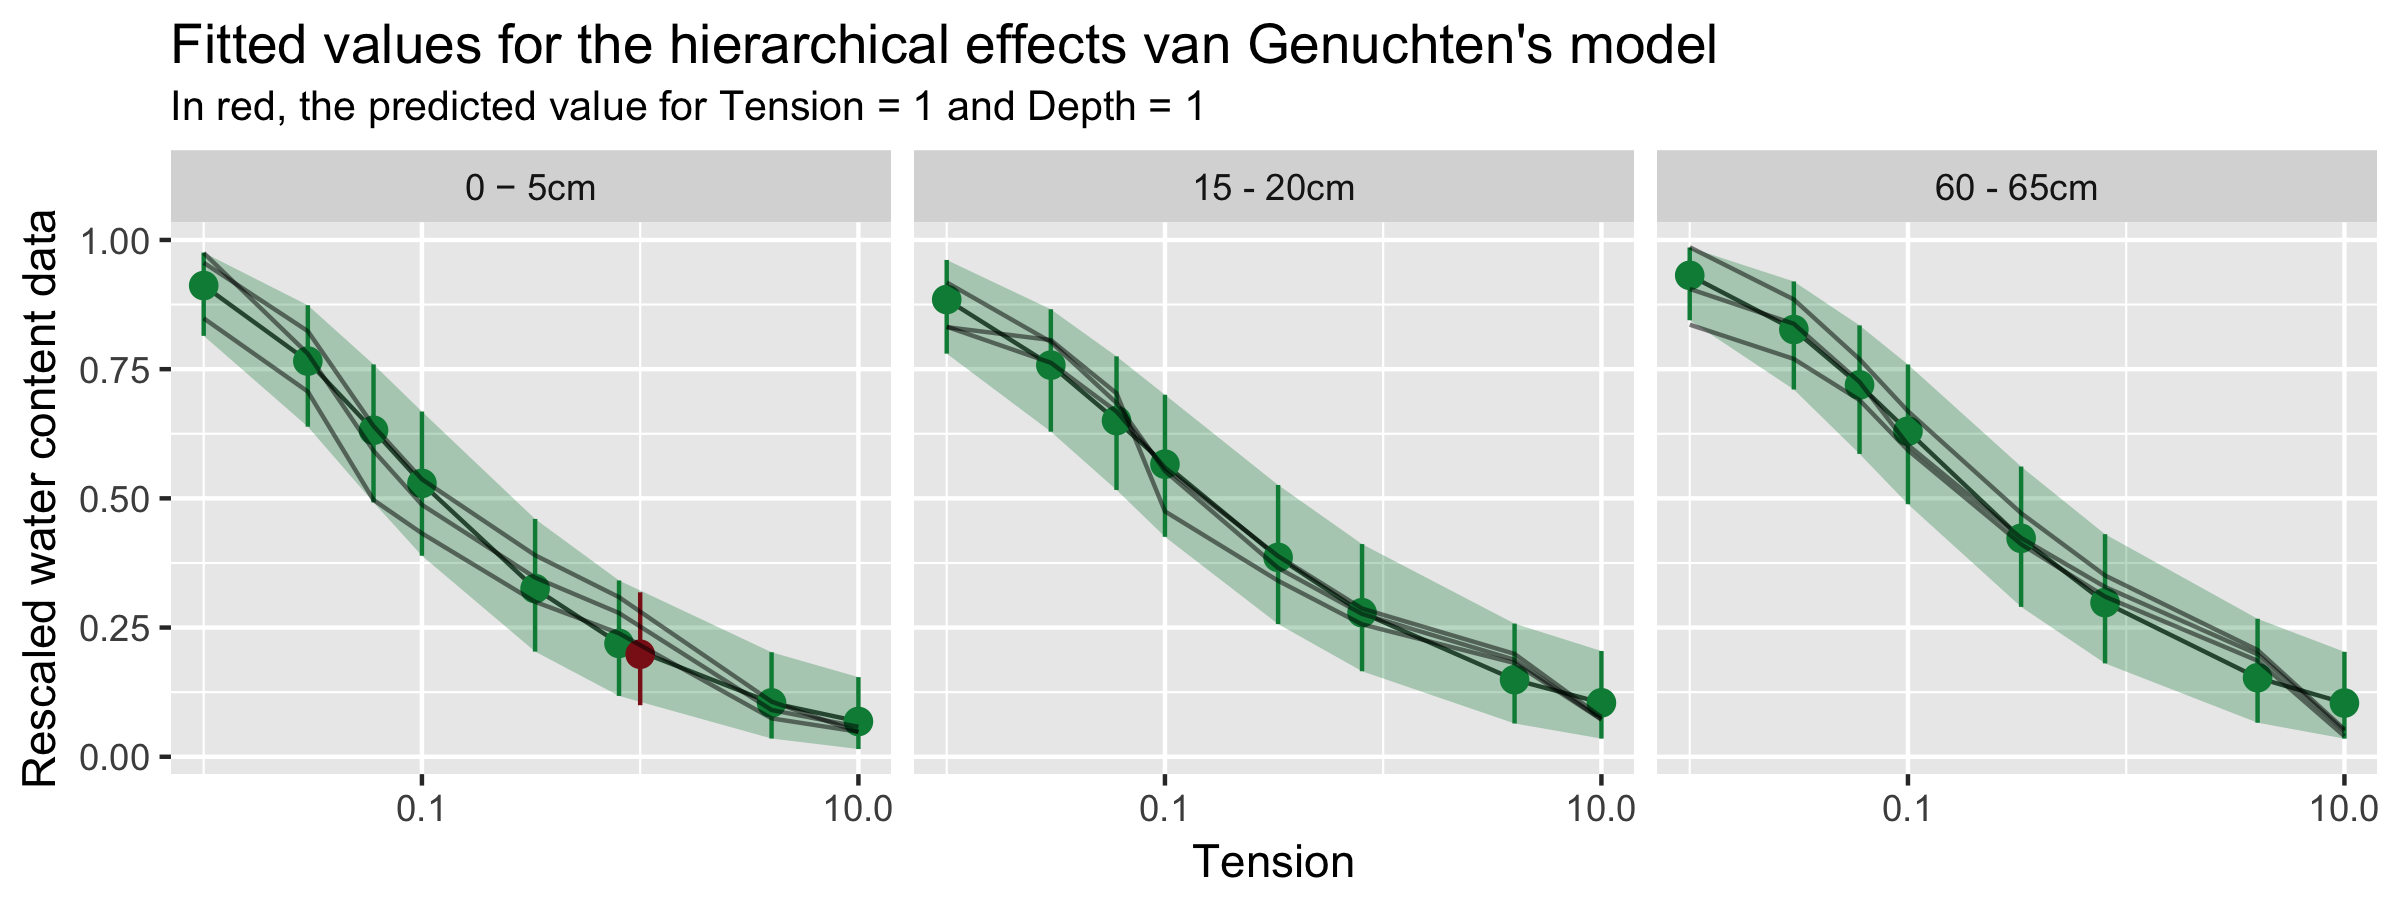
\includegraphics[width=16cm]{hier_3pars_pred.png}
\end{figure}

\subsubsection*{\underline{Convergence and autocorrelation}}
\begin{minipage}{0.50\textwidth}
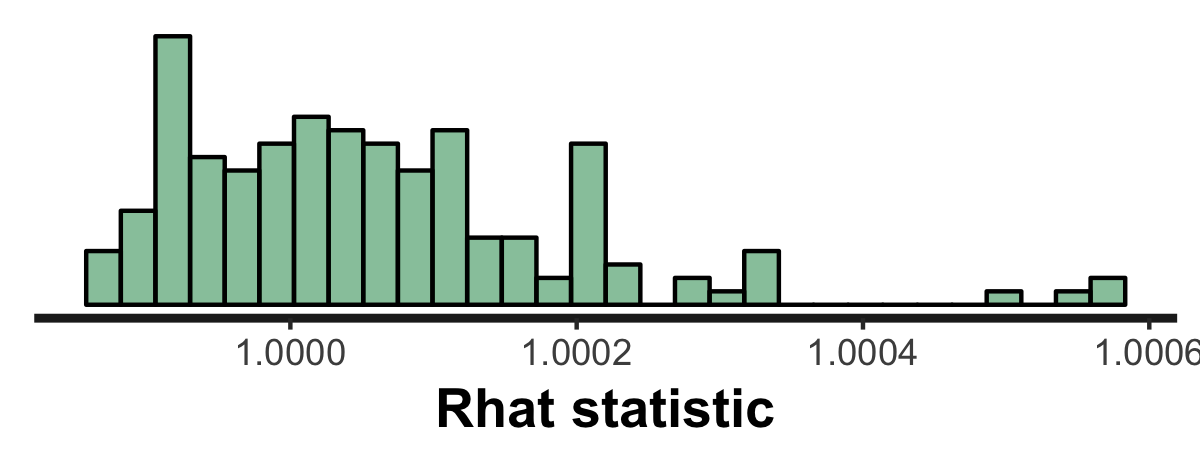
\includegraphics[width=\linewidth]{hier_3pars_rhat.png}
\end{minipage}
\begin{minipage}{0.50\textwidth}
Here is the histogram of the $\widehat{R}$ statistic. All values are close to 1: no problem of convergence. In addition, the autocorrelation plots in the Appendix A does not show any problem.
\end{minipage}

\subsubsection*{\underline{Posterior summaries}}
The below graph show the posterior distribution density for the parameters $\beta_1$, $\beta_2$, $\beta_3$ $\phi$ and $y_{pred}$. In addition, the posterior summaries are given. As can be seen, now there is one estimate of $\beta_1,\beta_2,\beta_3$ per depth. Also, the hyperparameters estimates for each $beta_1, beta_2, beta_3$ are shown (alpha1, alpha2, alpha3, beta1,beta2, beta3).
\begin{minipage}{0.50\textwidth}
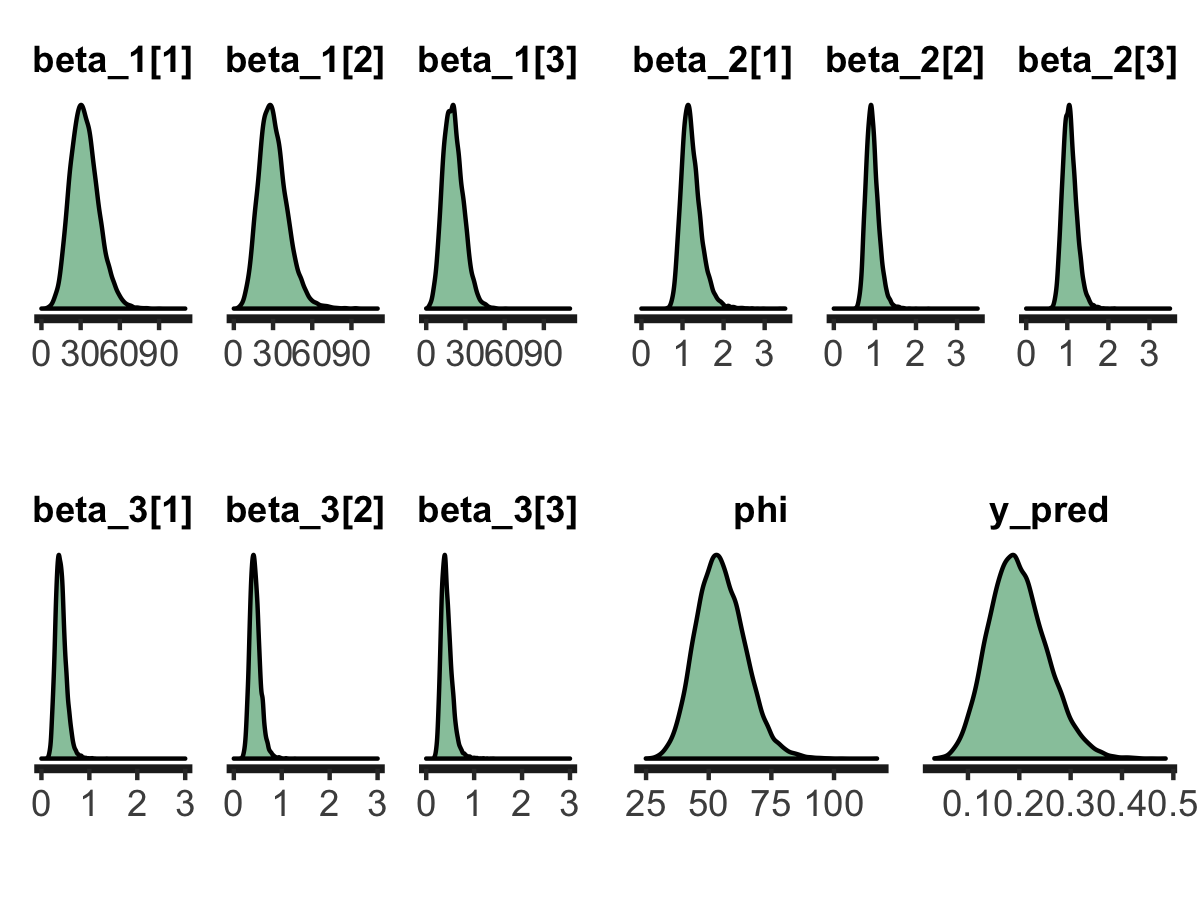
\includegraphics[width=\linewidth]{hier_3pars_dens.png}
\end{minipage}
\begin{minipage}{0.50\textwidth}
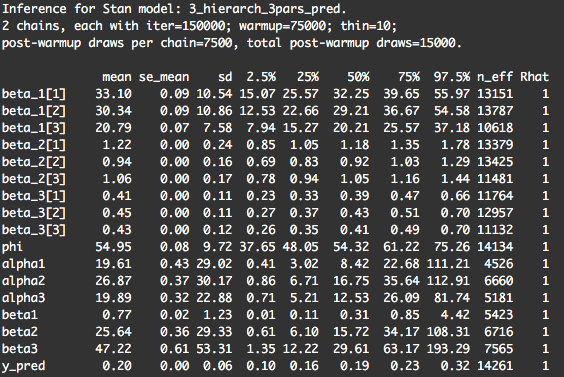
\includegraphics[width=\linewidth]{p06.png}
\end{minipage}


% %%%%%%%%%%%%%%%%%%%%%%%%%%%%%%%%%%%%%%%%%%%%%%%%%%%%%%%%%%%%%%%%%%%%%%%%%%%%%%%%%%%%%%%%%%%%
% %%%%%%%%%%%%%%%%%%%%%%%%%%%%%%%%%%%%%%%%%%%%%%%%%%%%%%%%%%%%%%%%%%%%%%%%%%%%%%%%%%%%%%%%%%%%
% %%%%%%%%%%%%%%%%%%%%%%%%%%%%%%%%%%%%%%%%%%%%%%%%%%%%%%%%%%%%%%%%%%%%%%%%%%%%%%%%%%%%%%%%%%%%
% %%%%%%%%%%%%%%%%%%%%%%%%%%%%%%%%%%%%%%%%%%%%%%%%%%%%%%%%%%%%%%%%%%%%%%%%%%%%%%%%%%%%%%%%%%%%

\newpage
\section{Model selection}

Stan does not provide the DIC directly. The reasons about this decision are written on the STAN-users mailing group \footnote{https://groups.google.com/forum/\#!topic/stan-users/SbdA47xC4Fw}. There is an open discussion about the benefits of different measures, but until now, they prefer other measures like WAIC and LOO (Leave-One-Out Cross-Validation).

As these measures require to compute the log point-wise predictive density, a piece of code is included in each stan file. After that, following the example of \cite{vehtari2016practical}, I compute the WAIC for each model (using the package loo \cite{loo}):


\begin{table}[ht!]
\centering
\caption{Comparison of WAIC}
\label{my-label}
\begin{tabular}{lll}
Model                                    & \begin{tabular}[c]{@{}l@{}}Estimate\\ $elpd_{waic}$\end{tabular} & \begin{tabular}[c]{@{}l@{}}Estimate\\ $p_{waic}$\end{tabular} \\ \hline
Pooled-effects Gardner model             & 95.7                                                            & 3.7                                                        \\
Pooled-effects van Genuchten model       & 100.0                                                           & 4.9                                                        \\
Independent-effects Gardner model        & 101.0                                                           & 8.1                                                        \\
Independent-effects van Genuchten model  & 105.3                                                           & 13.5                                                       \\
Hierarchical-effects Gardner model       & 101.1                                                           & 7.3                                                        \\
Hierarchical-effects van Genuchten model & 106.6                                                           & 10.3                                                      
\end{tabular}
\end{table}

We have the equality $\widehat{elpd}_{waic} = \widehat{lpd}$ - $\widehat{p}_{waic}$, with $\widehat{lpd}$ a \say{measure of predictive accuracy}, and $\widehat{p}_{waic}$ the \say{estimated effective number of parameters.}. Then, for these model and the data provided, the Hierarchical-effects van Genuchten model is the preferred.


\section{Prior sensitivity analysis}

\subsection*{Change in the prior of $\phi$}
To analyze the prior sensitivity for this parameter, a gamma prior distribution with shape ans scale parameters equal to $0.01$, and a uniform distribution between in the interval $[0, 100]$ for the parameter $\phi$ will be compared:

\begin{figure}[ht!]
\centering
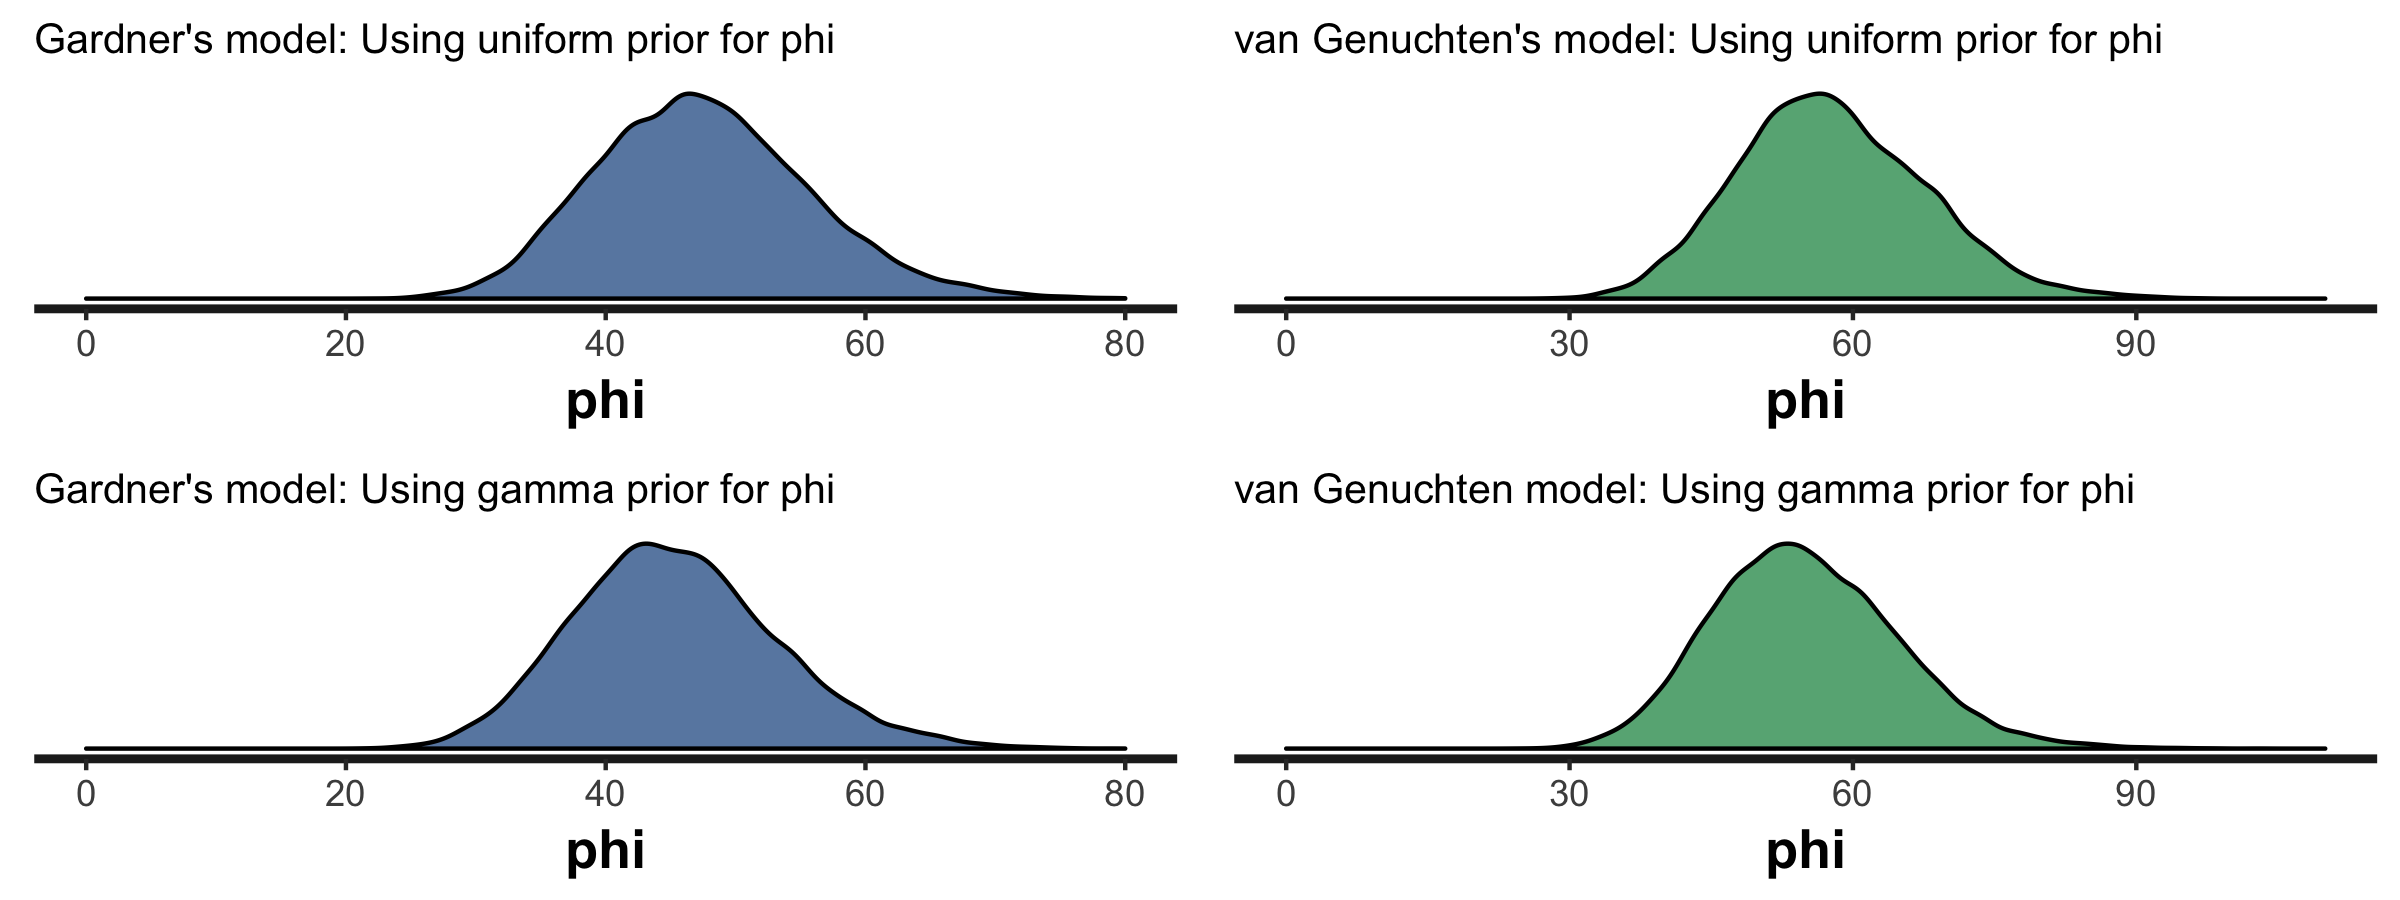
\includegraphics[width=13cm]{sens_1.png}
\end{figure}

Observing the above graph, for this change of priors, there is no important change in the posterior distribution of $\phi$.
\newpage
\subsection*{Change in the prior of the hyperparameters of each $\beta_i$, $i = 1,2,3$.}
Now, the selected model uses prior distributions in the hyperparameters of each $\beta$. In the first experiment, these a priori distributions were uninformative gamma distributions with parameters $\alpha = 0.01, \beta = 0.01$. Now, uniform distributions from 0 to 100 were used.

\begin{figure}[ht!]
\centering
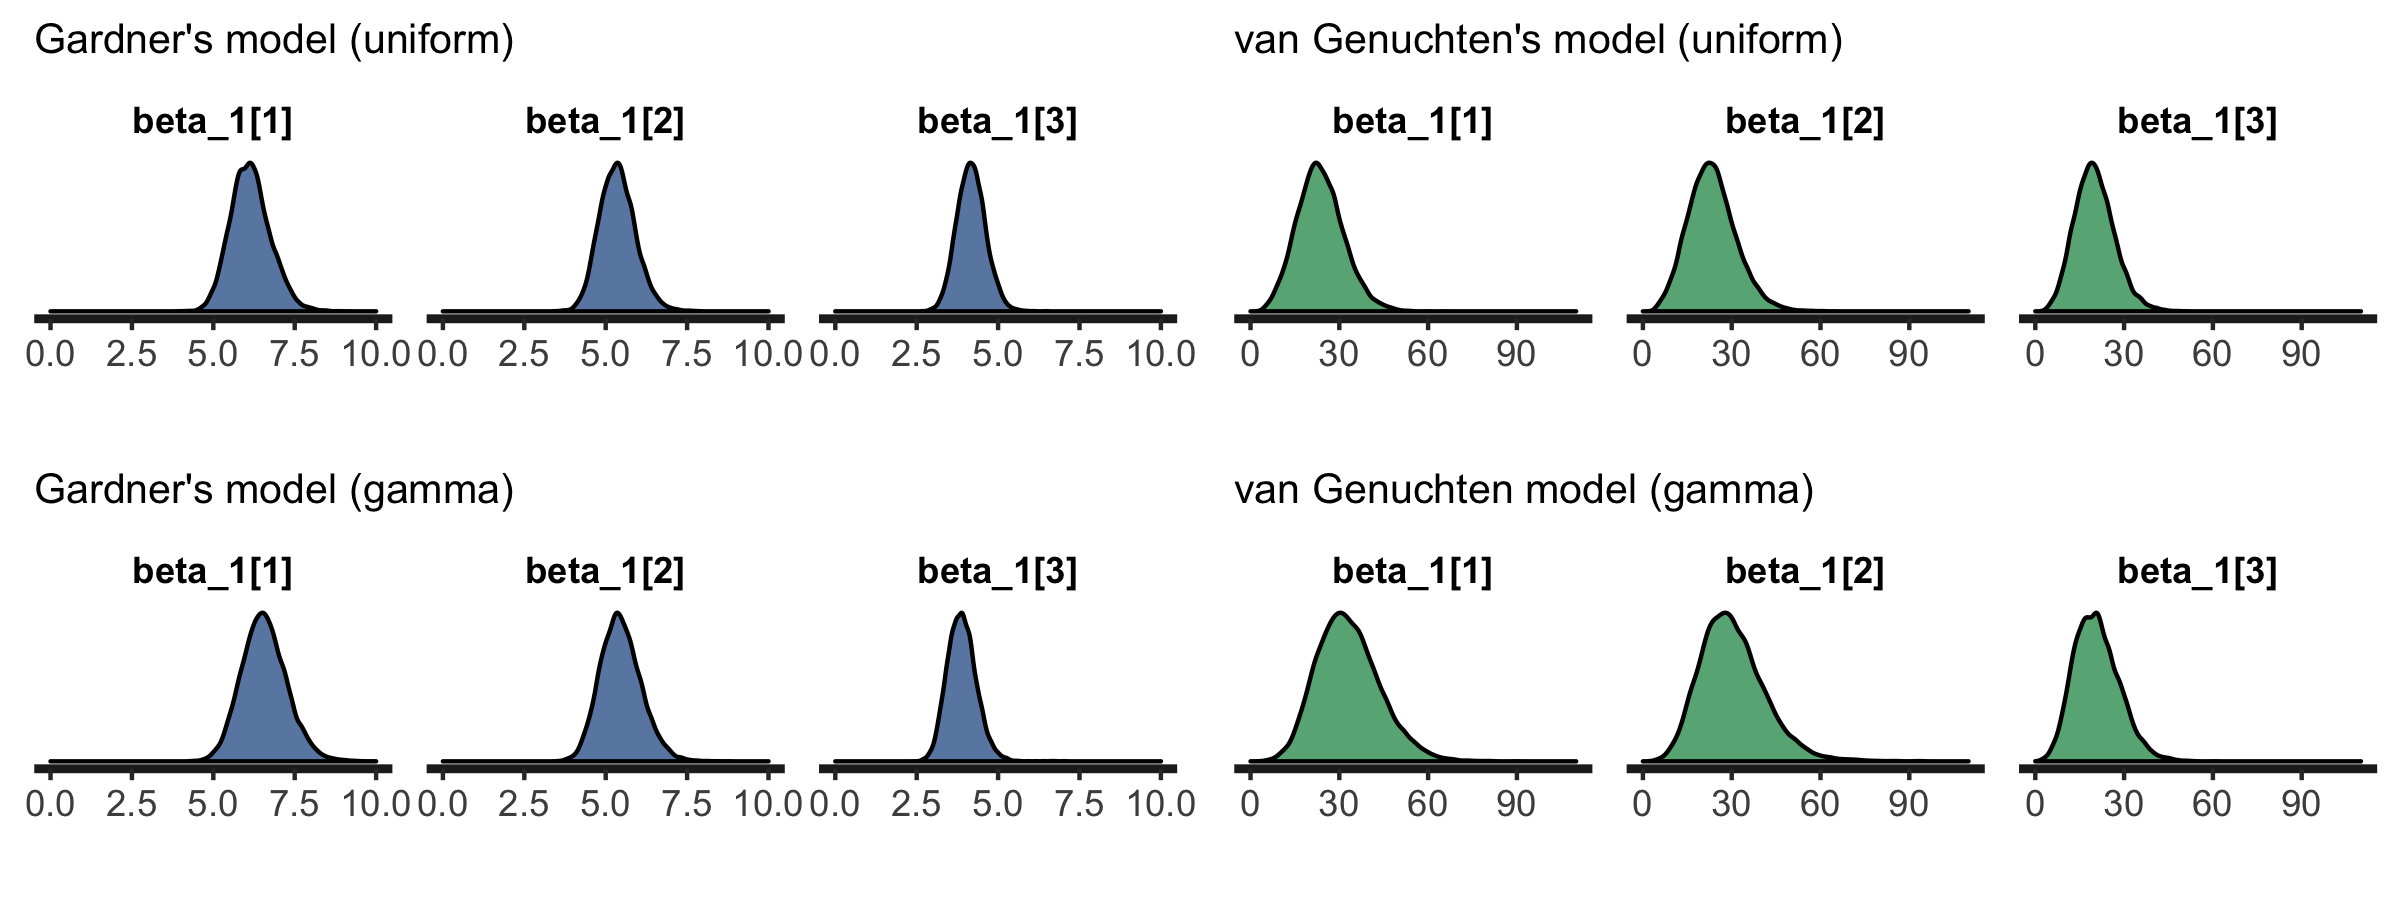
\includegraphics[width=16cm]{sens_2.png}
\end{figure}

\begin{figure}[ht!]
\centering
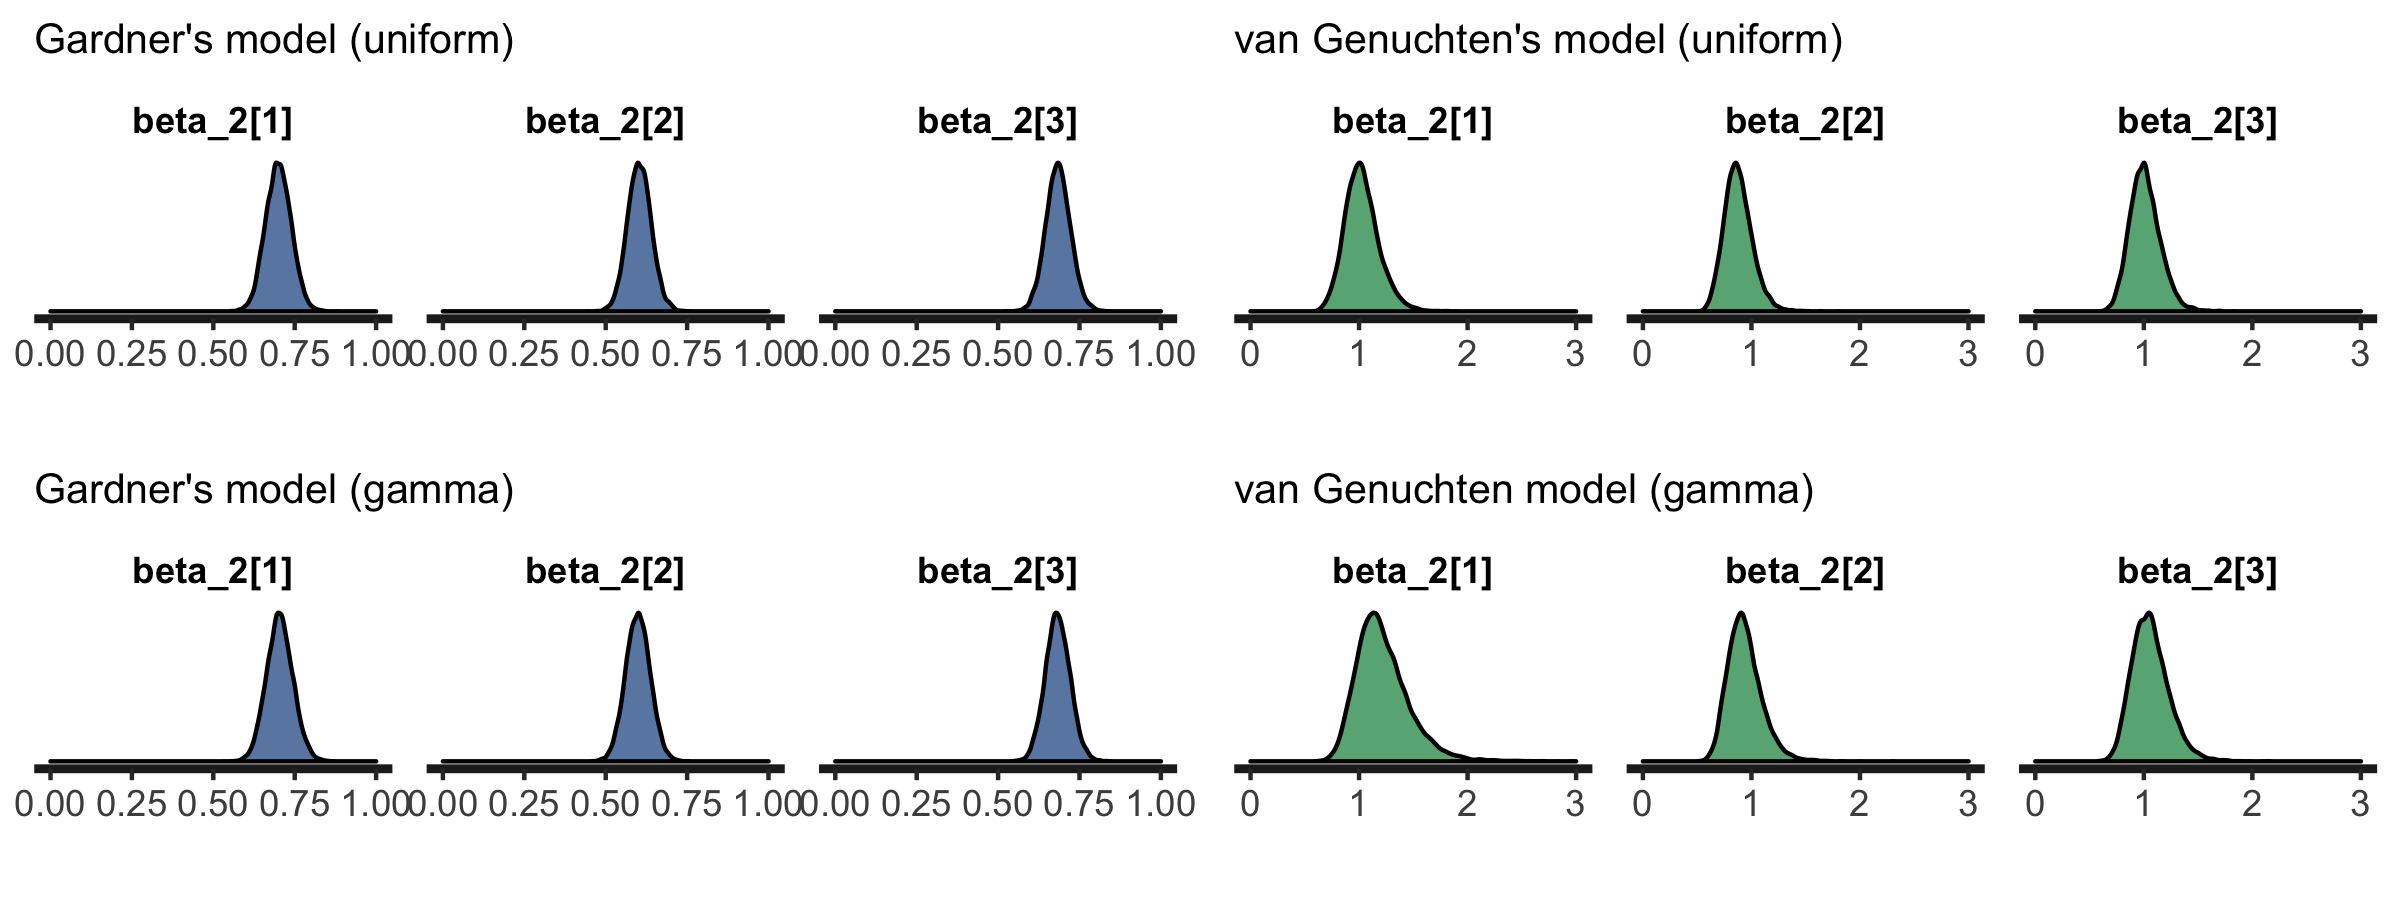
\includegraphics[width=16cm]{sens_3.png}
\end{figure}

\begin{figure}[ht!]
\centering
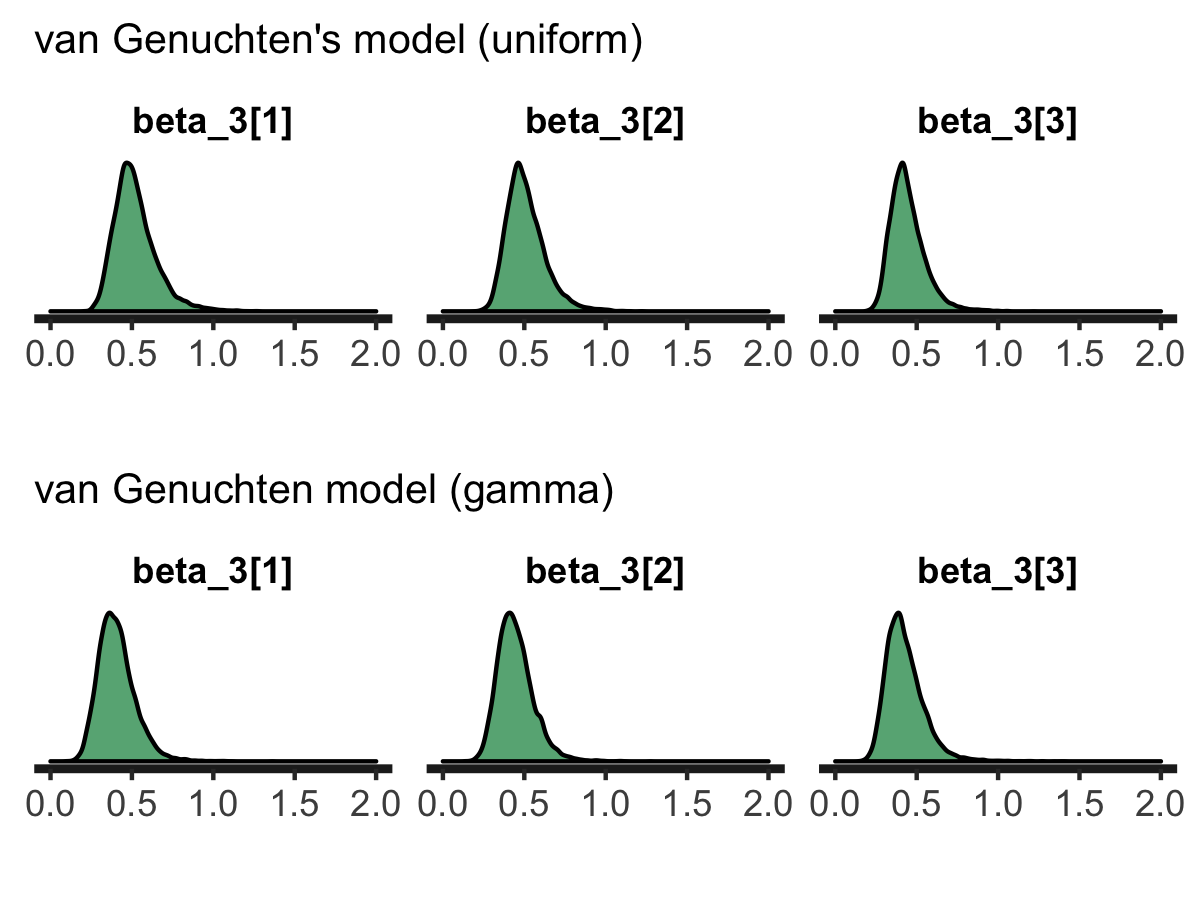
\includegraphics[width=8cm]{sens_4.png}
\end{figure}

In these graphs we can see a slightly movement of the posterior distributions, but the shape and domain is almost the same for all of them. 
\newpage
\subsection*{Change in the predictive posterior distribution}
To assess is there is a change in the predictive posterior distribution when specifying distinct prior distributions, the posterior plots are shown in the graphs below:


\begin{minipage}{0.50\textwidth}
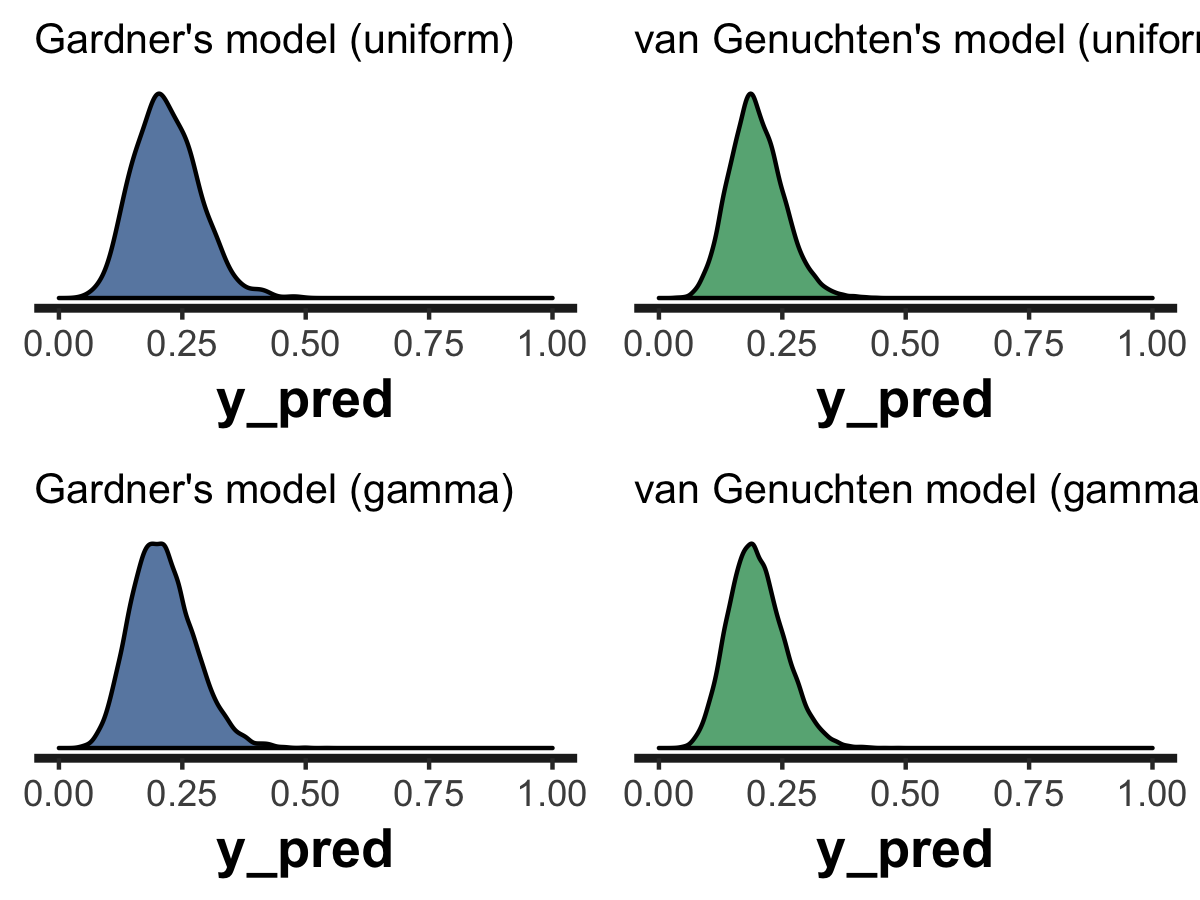
\includegraphics[width=\linewidth]{sens_pred.png}
\end{minipage}
\begin{minipage}{0.50\textwidth}
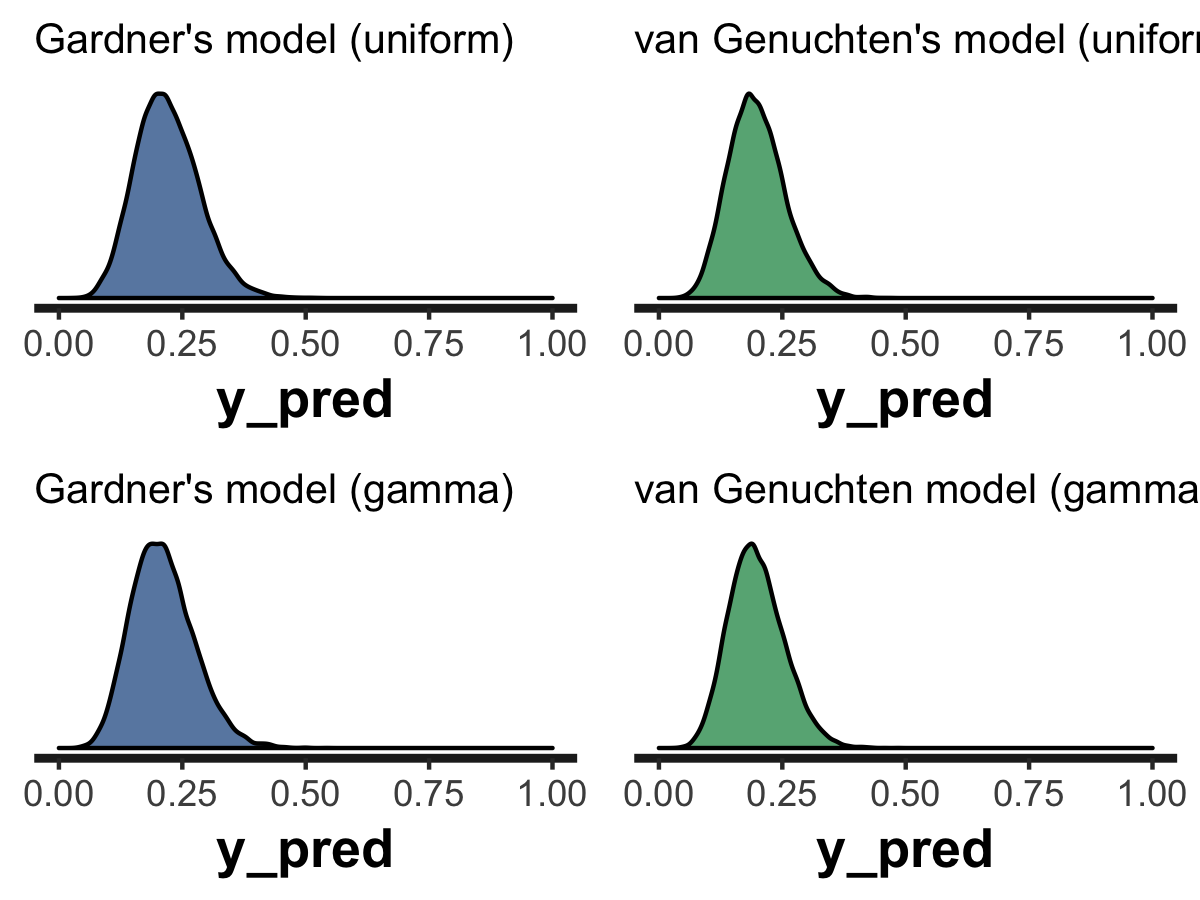
\includegraphics[width=\linewidth]{sens_pred2.png}
\end{minipage}

The four plots in the left shows the posterior plots of $y_{pred}$ when prior distribution for $\phi$ is changed. On the other hand, the four right plots shows the posterior plots of $y_{pred}$ when the prior distribution of the hyperparameters of $\beta_1, \beta_2, \beta_3$ are changed. As can be seen, the use of both priors provide similar posterior distributions.


\section{Conclusions and improvements to the model}


I have two ideas to improve this model. The first is to consider a hierarchical-effect of a subgroup of ${\beta_1, \beta_2, \beta_3}$, not of the three of them (as is made in the last section). As we are penalizing the WAIC with the effective number of parameters, less parameters can yield to a better result. The second idea is to try different models for $\phi$. In this report, I treated the $phi$ as a constant, but it can depend on the level of the depth (as the $\beta$'s parameters), or even as \cite{cribari2009beta} says, can have it's own model.

As the conclusions, the model that was the better in terms of WAIC was the hierarchical model with three parameters. In the final model there is evidence of variability in the data according to the depth level, for example, the mean of $\beta_1$ when depth = 1 is 33.10 and the mean of $\beta_1$ when depth = 3 is 20.79, a difference of more than 12 units (and this number is large compared with the sd of each parameter). In fact, a line of code can be added to the model to estimate the difference between the $\beta_1$ for different depths. This idea can help us to decide for which variables we should make pooling or consider a hierarchical model (In addition to the WAIC measure).
\newpage
\section{Appendix}
\subsection*{Appendix A: Pooled model}
\subsubsection*{\textbf{Gardner's model}}

\begin{figure}[ht!]
\centering
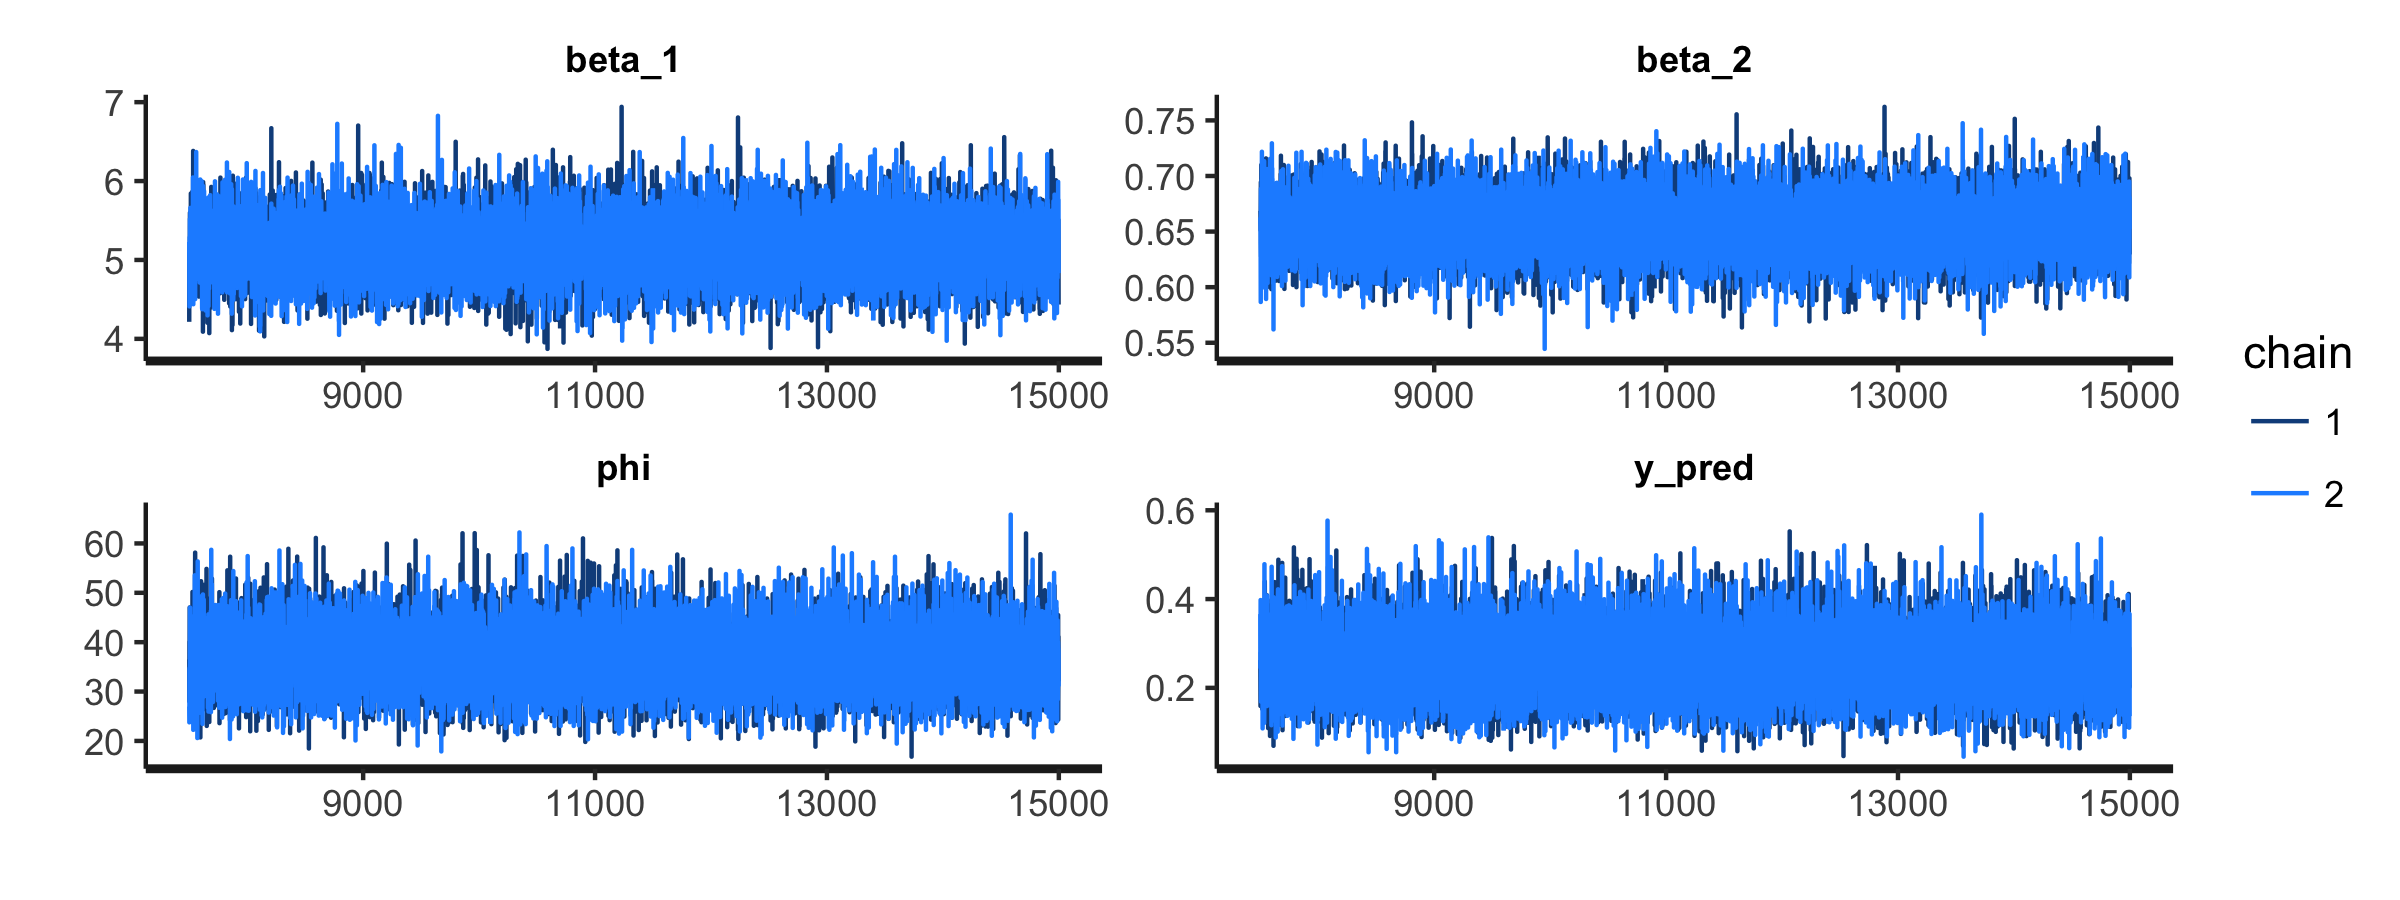
\includegraphics[width=16cm, height = 5 cm]{pooled_2pars_trace.png}
\end{figure}

\begin{figure}[ht!]
\centering
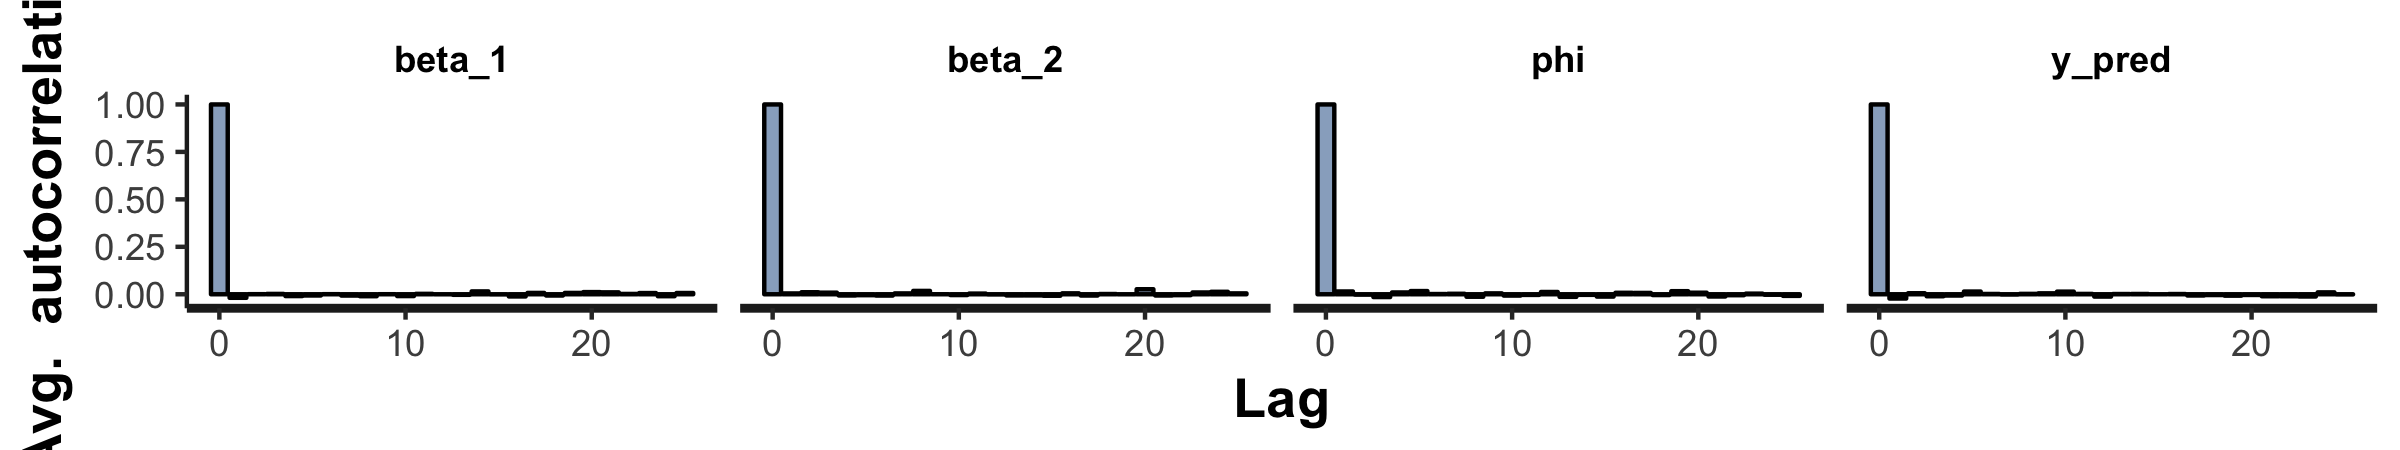
\includegraphics[width=16cm]{pooled_2pars_ac.png}
\end{figure}

\subsubsection*{van Genuchten model}

\begin{figure}[ht!]
\centering
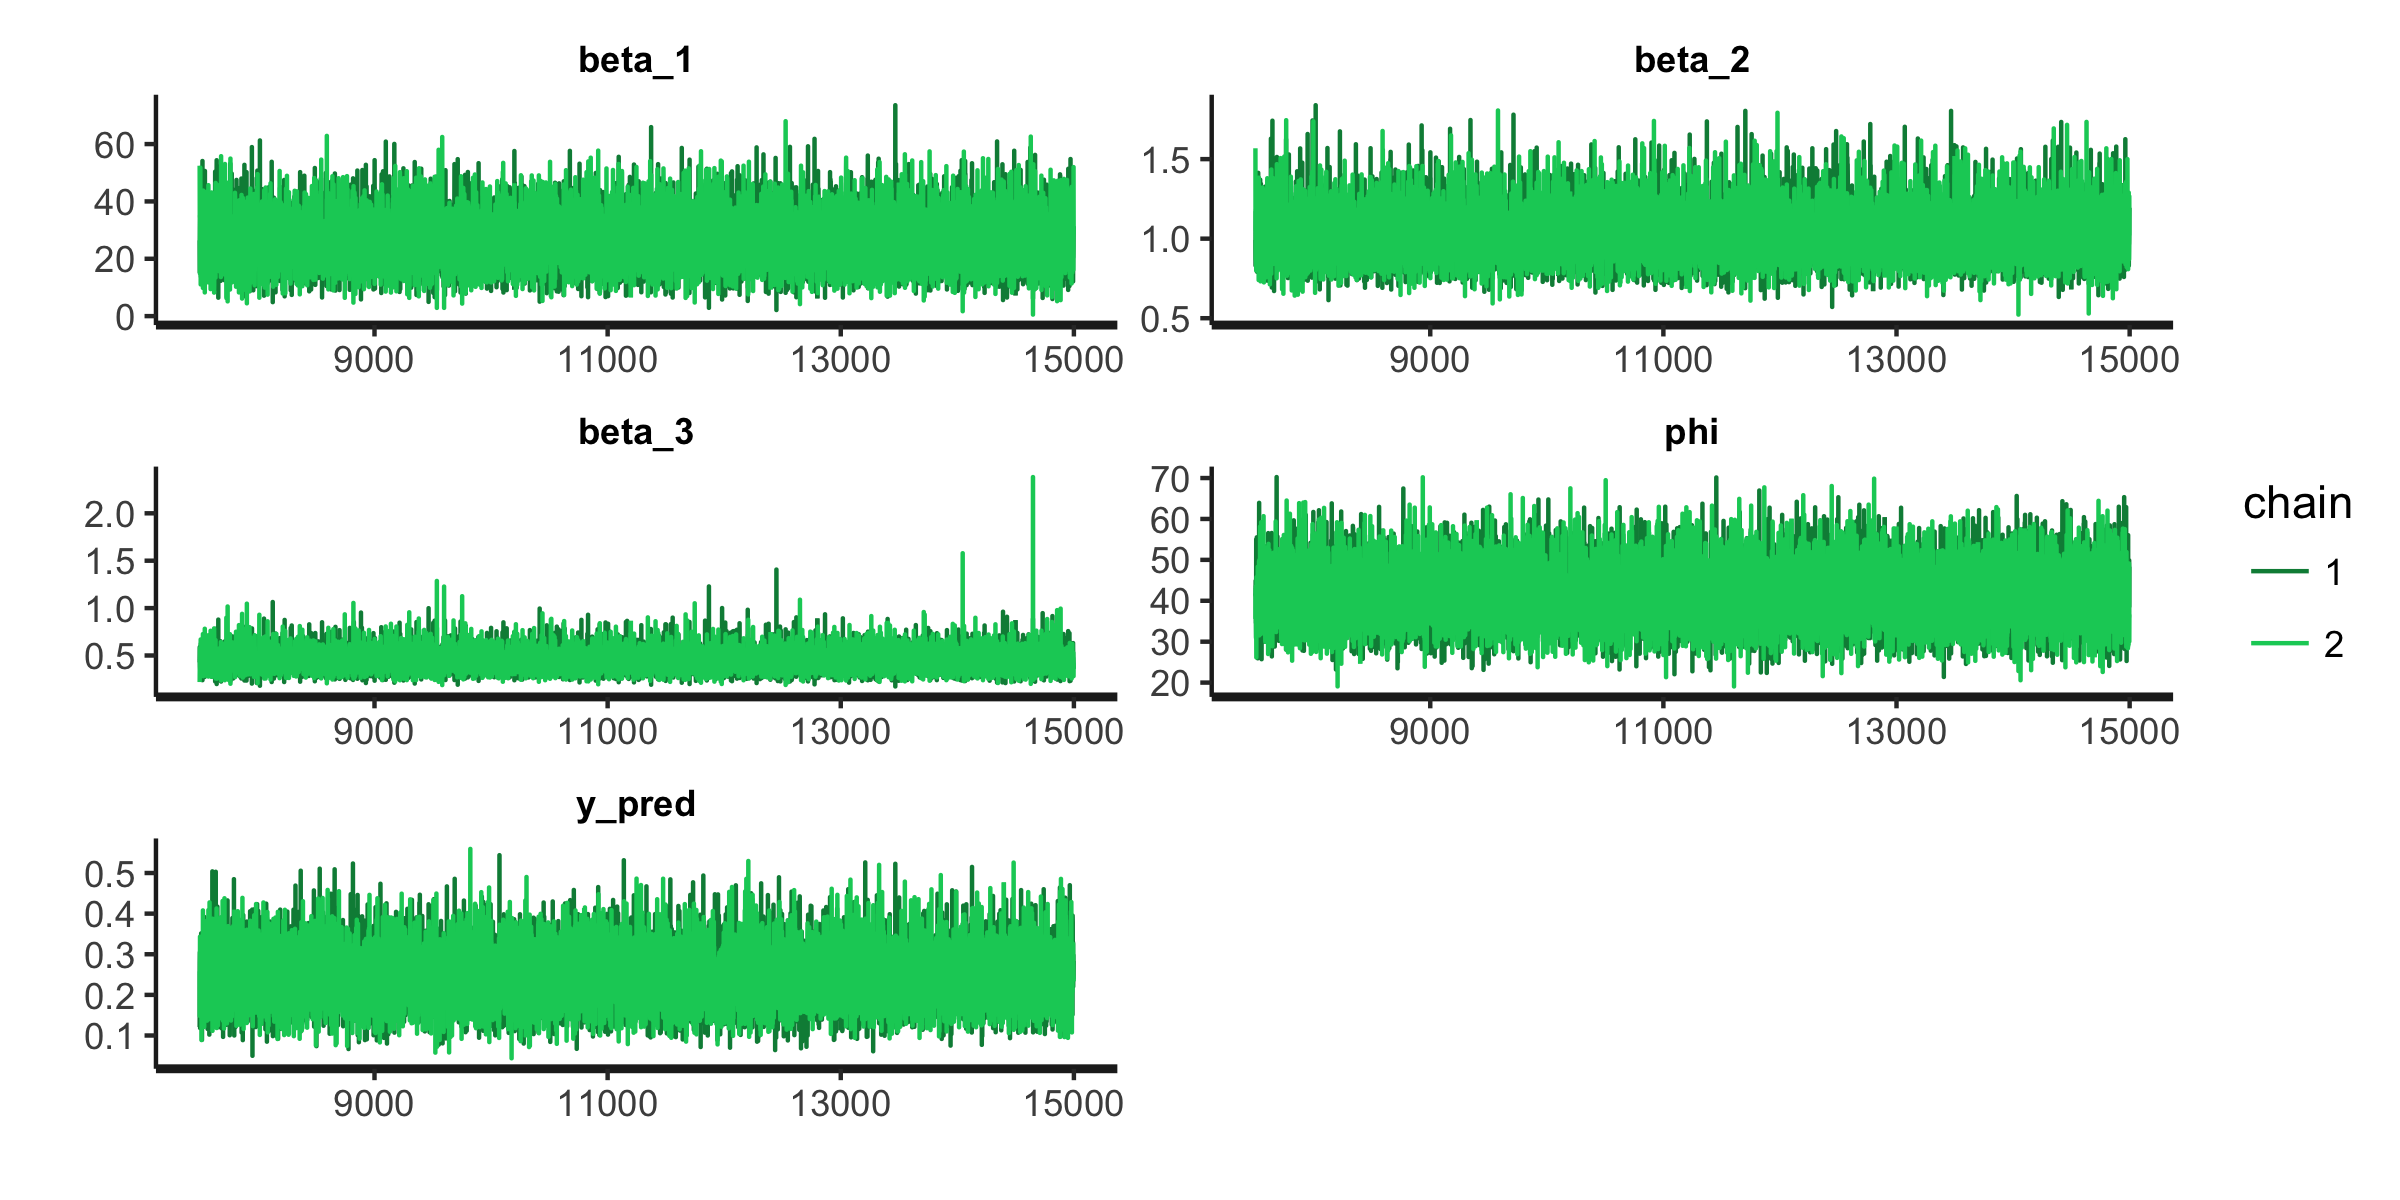
\includegraphics[width=16cm, height = 5 cm]{pooled_3pars_trace.png}
\end{figure}

\begin{figure}[ht!]
\centering
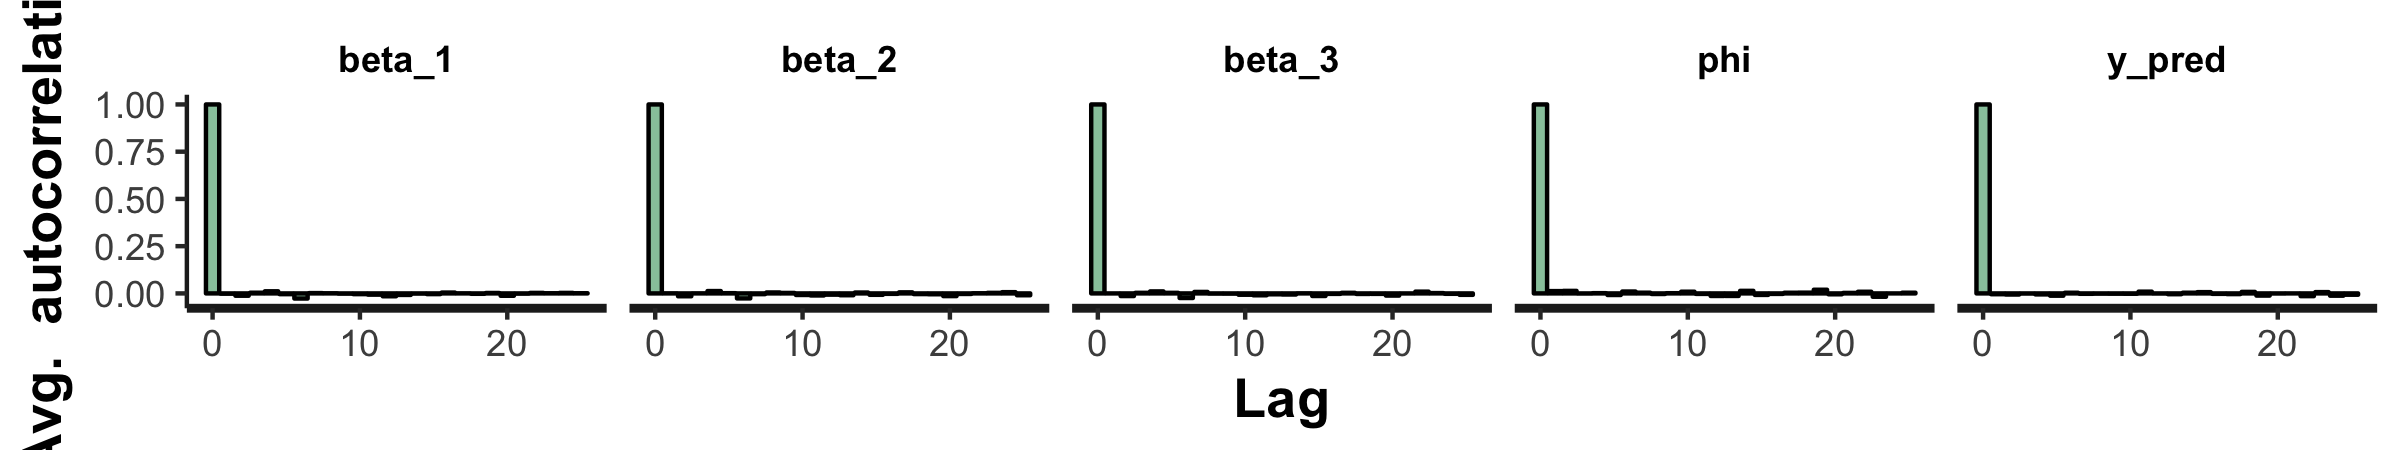
\includegraphics[width=16cm]{pooled_3pars_ac.png}
\end{figure}

\subsection*{Appendix B: Independent effects model}
\subsubsection*{\textbf{Gardner's model}}

\begin{figure}[ht!]
\centering
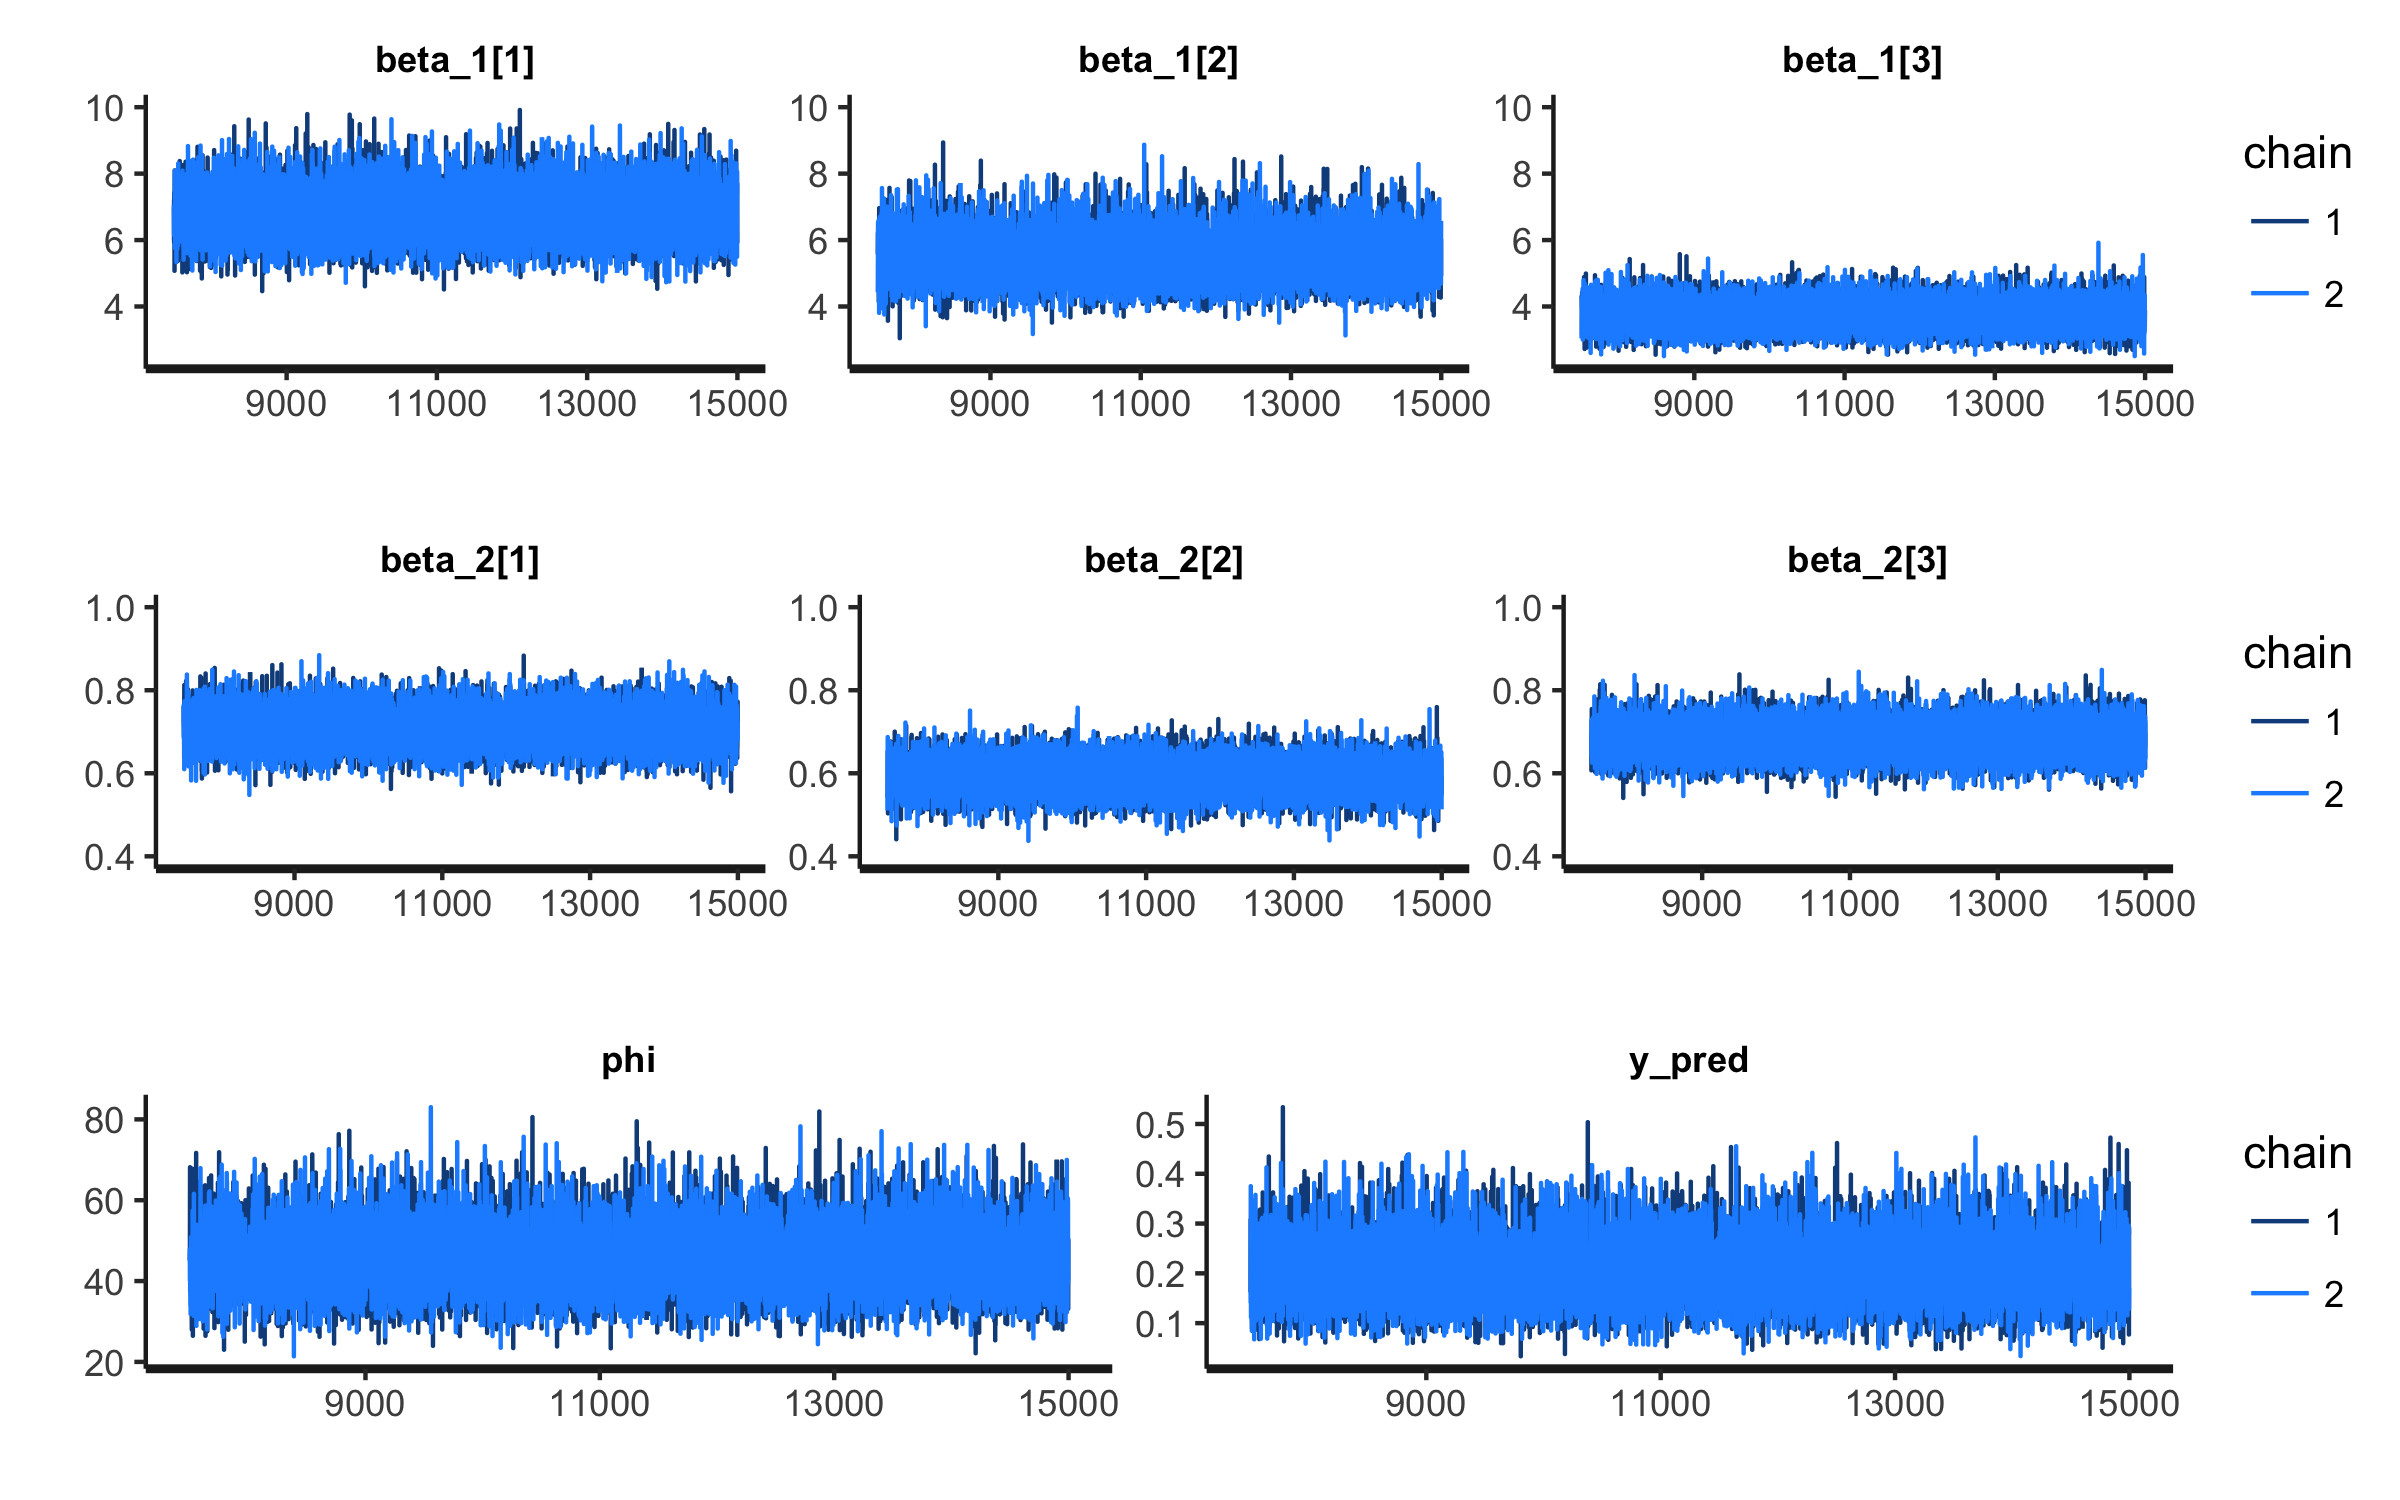
\includegraphics[width=16cm]{indep_2pars_trace.png}
\end{figure}

\begin{figure}[ht!]
\centering
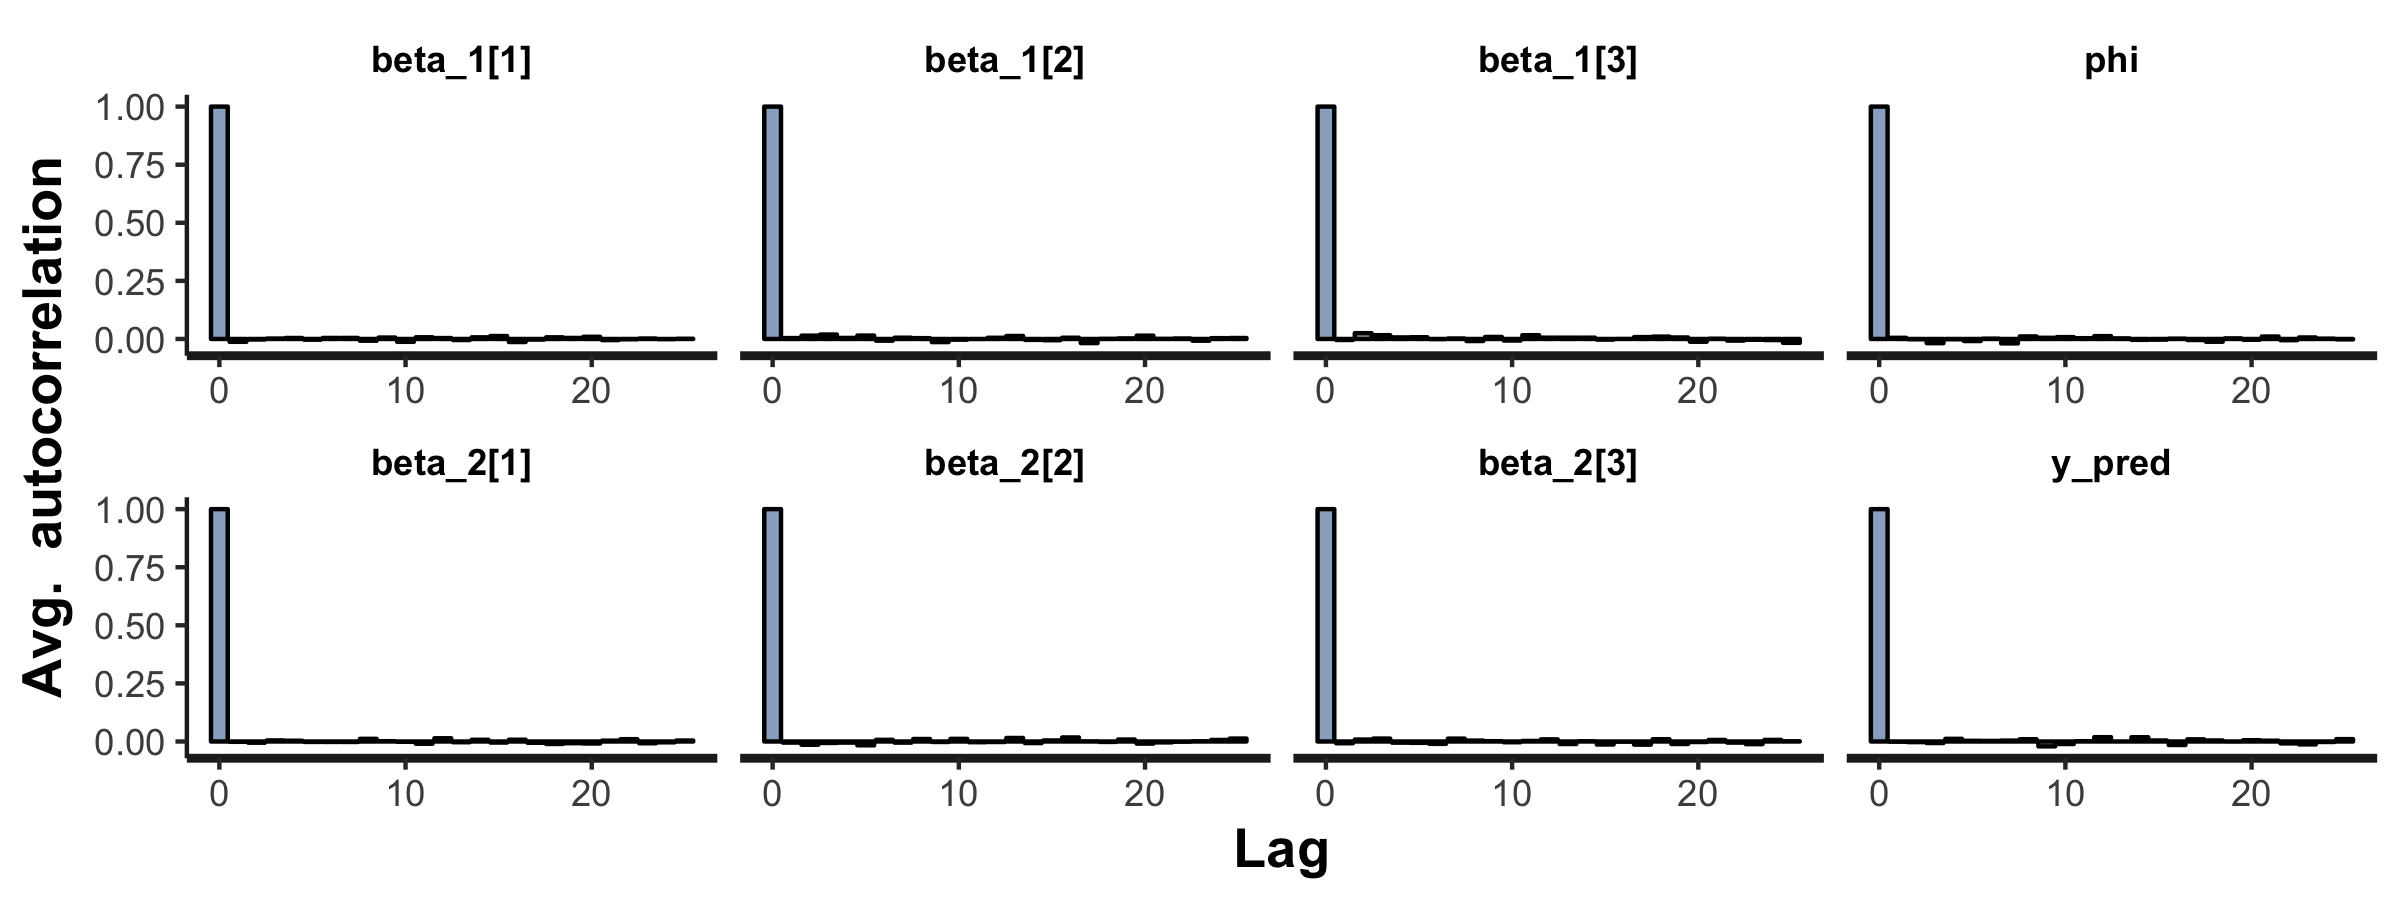
\includegraphics[width=16cm]{indep_2pars_ac.png}
\end{figure}

\newpage
\subsubsection*{van Genuchten model}
\begin{figure}[ht!]
\centering
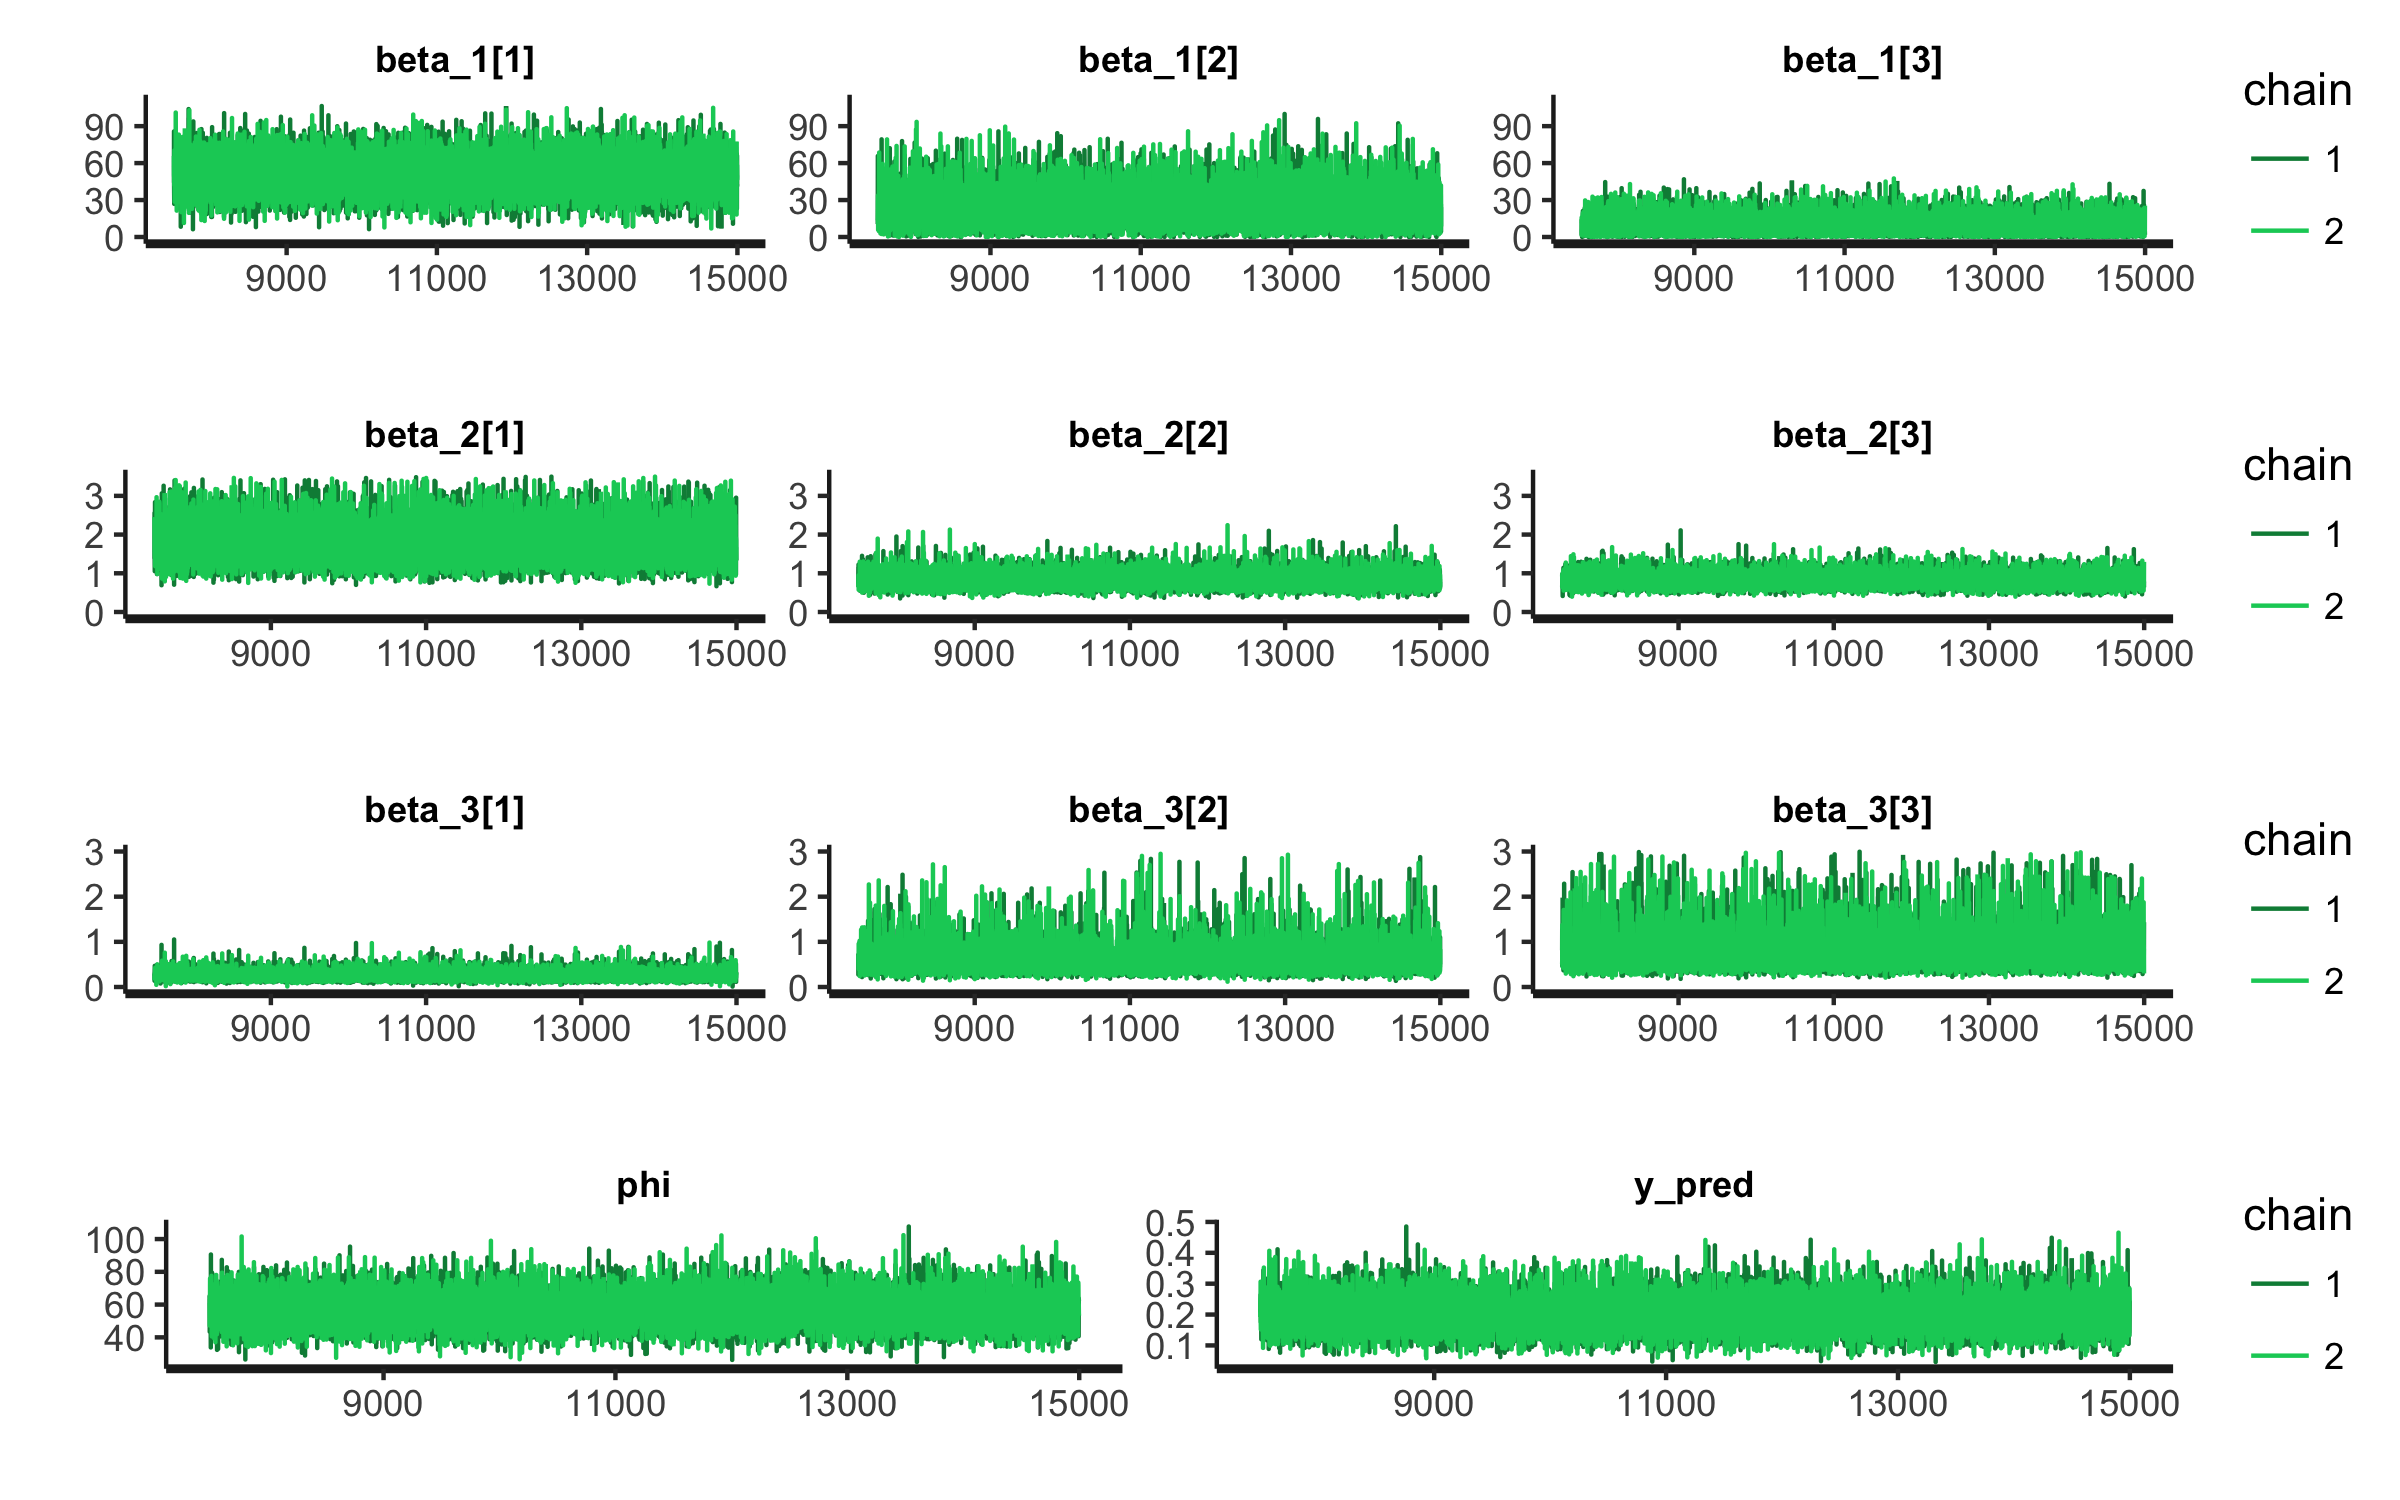
\includegraphics[width=16cm]{indep_3pars_trace.png}
\end{figure}

\begin{figure}[ht!]
\centering
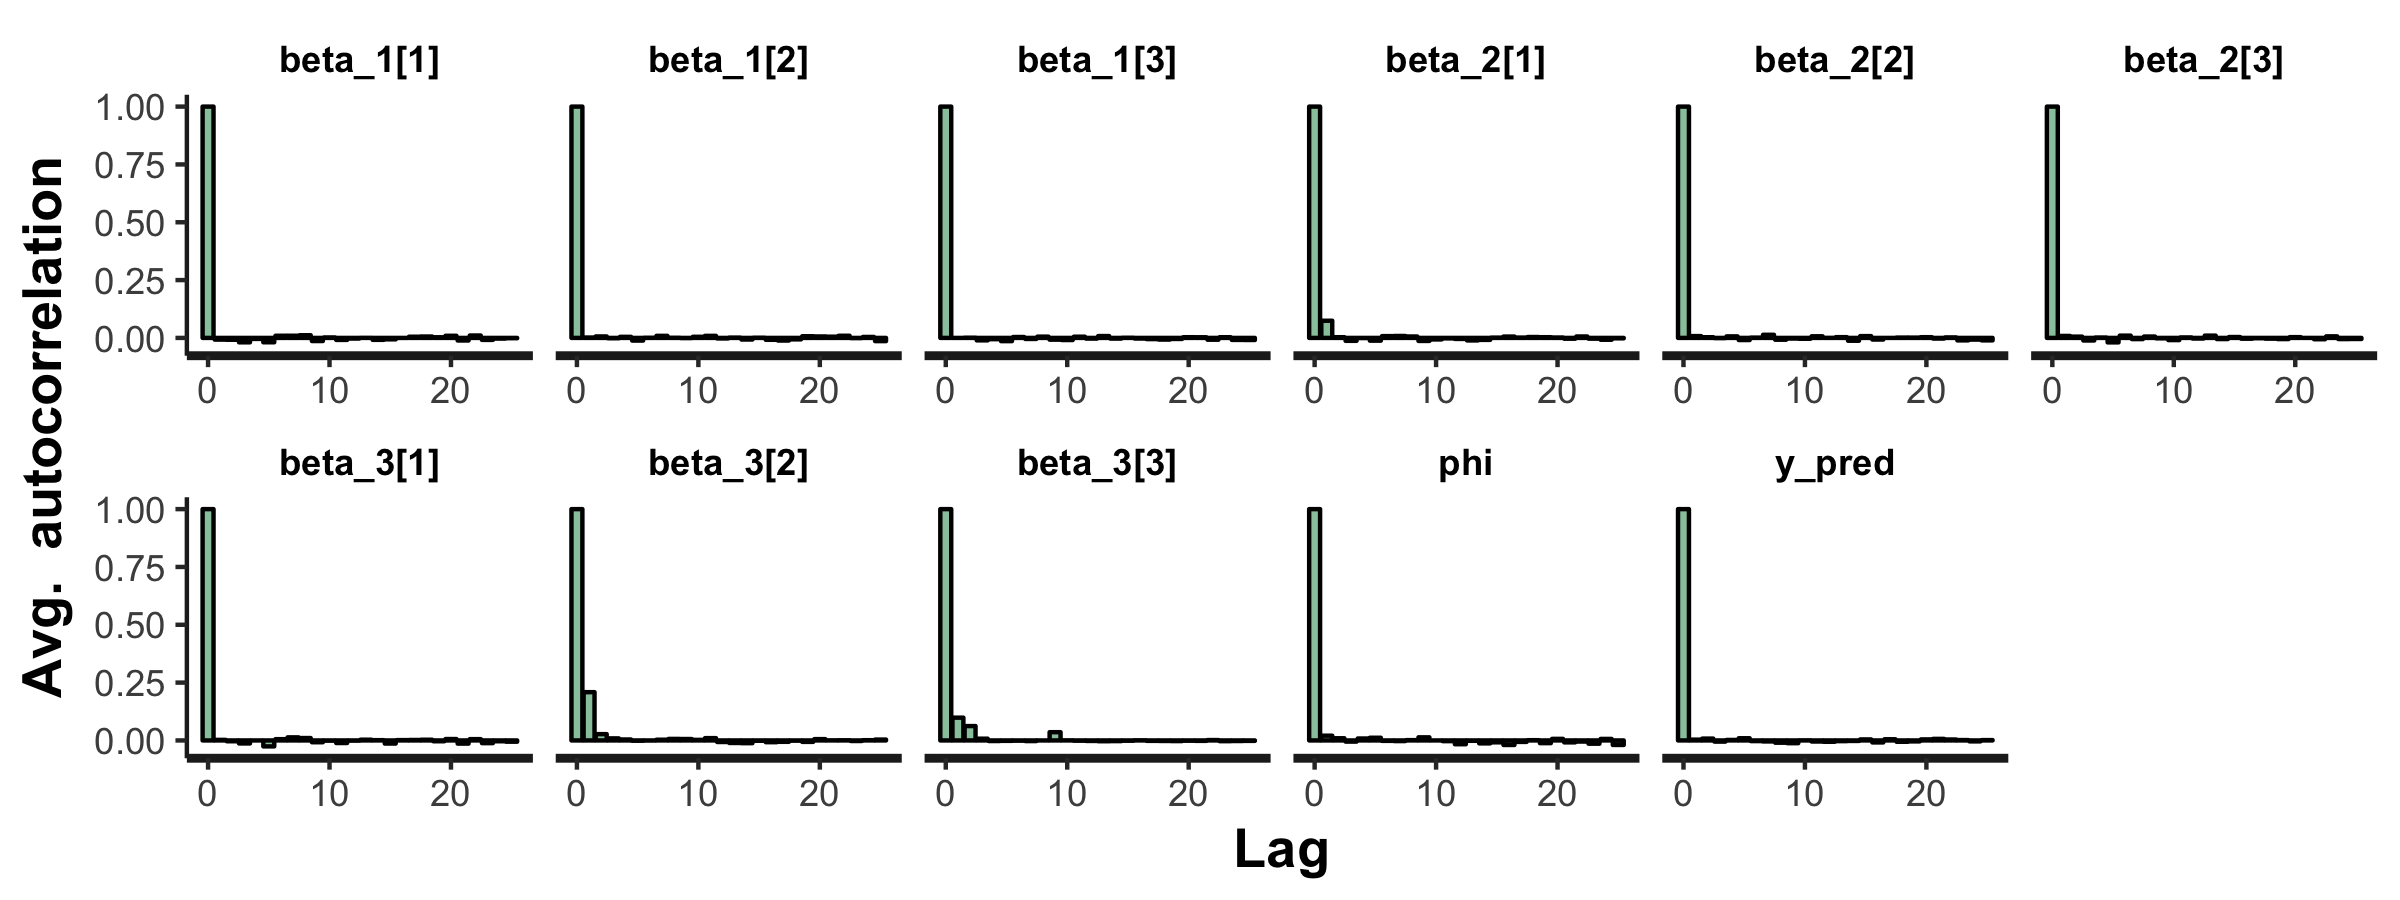
\includegraphics[width=16cm]{indep_3pars_ac.png}
\end{figure}

\newpage
\subsection*{Appendix C: Hierarchical model}
\subsubsection*{\textbf{Gardner's model}}
\begin{figure}[ht!]
\centering
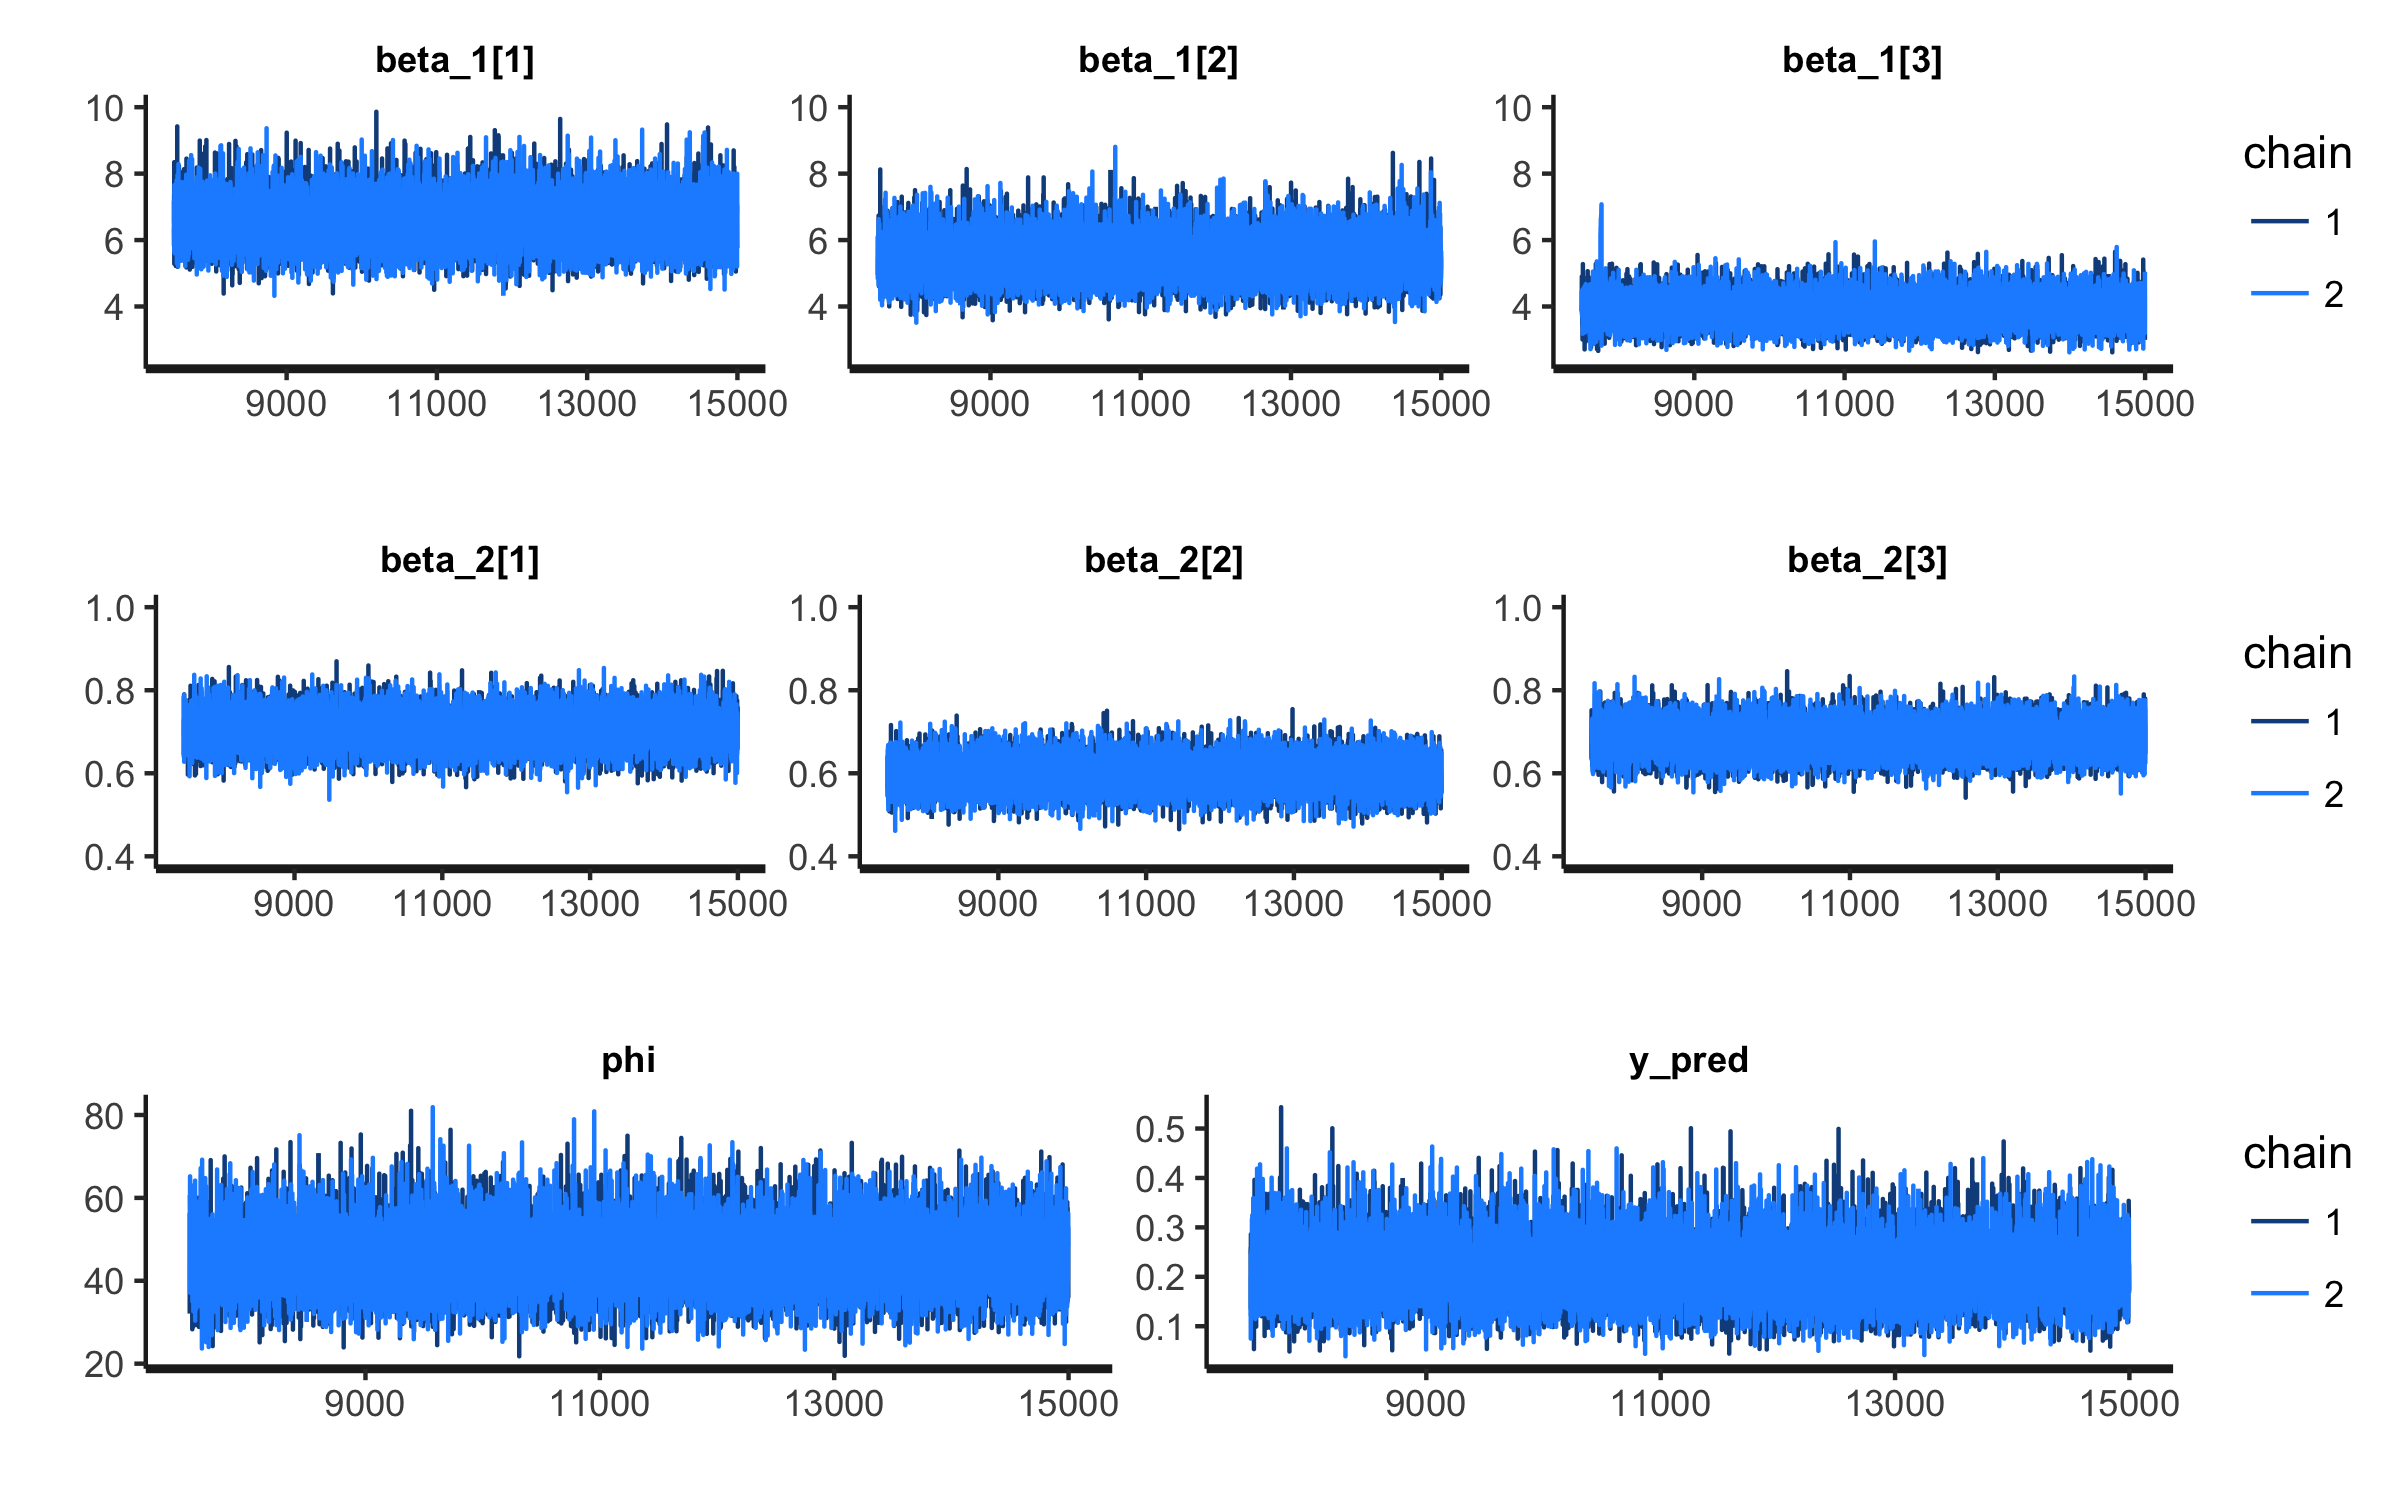
\includegraphics[width=16cm]{hier_2pars_trace.png}
\end{figure}

\begin{figure}[ht!]
\centering
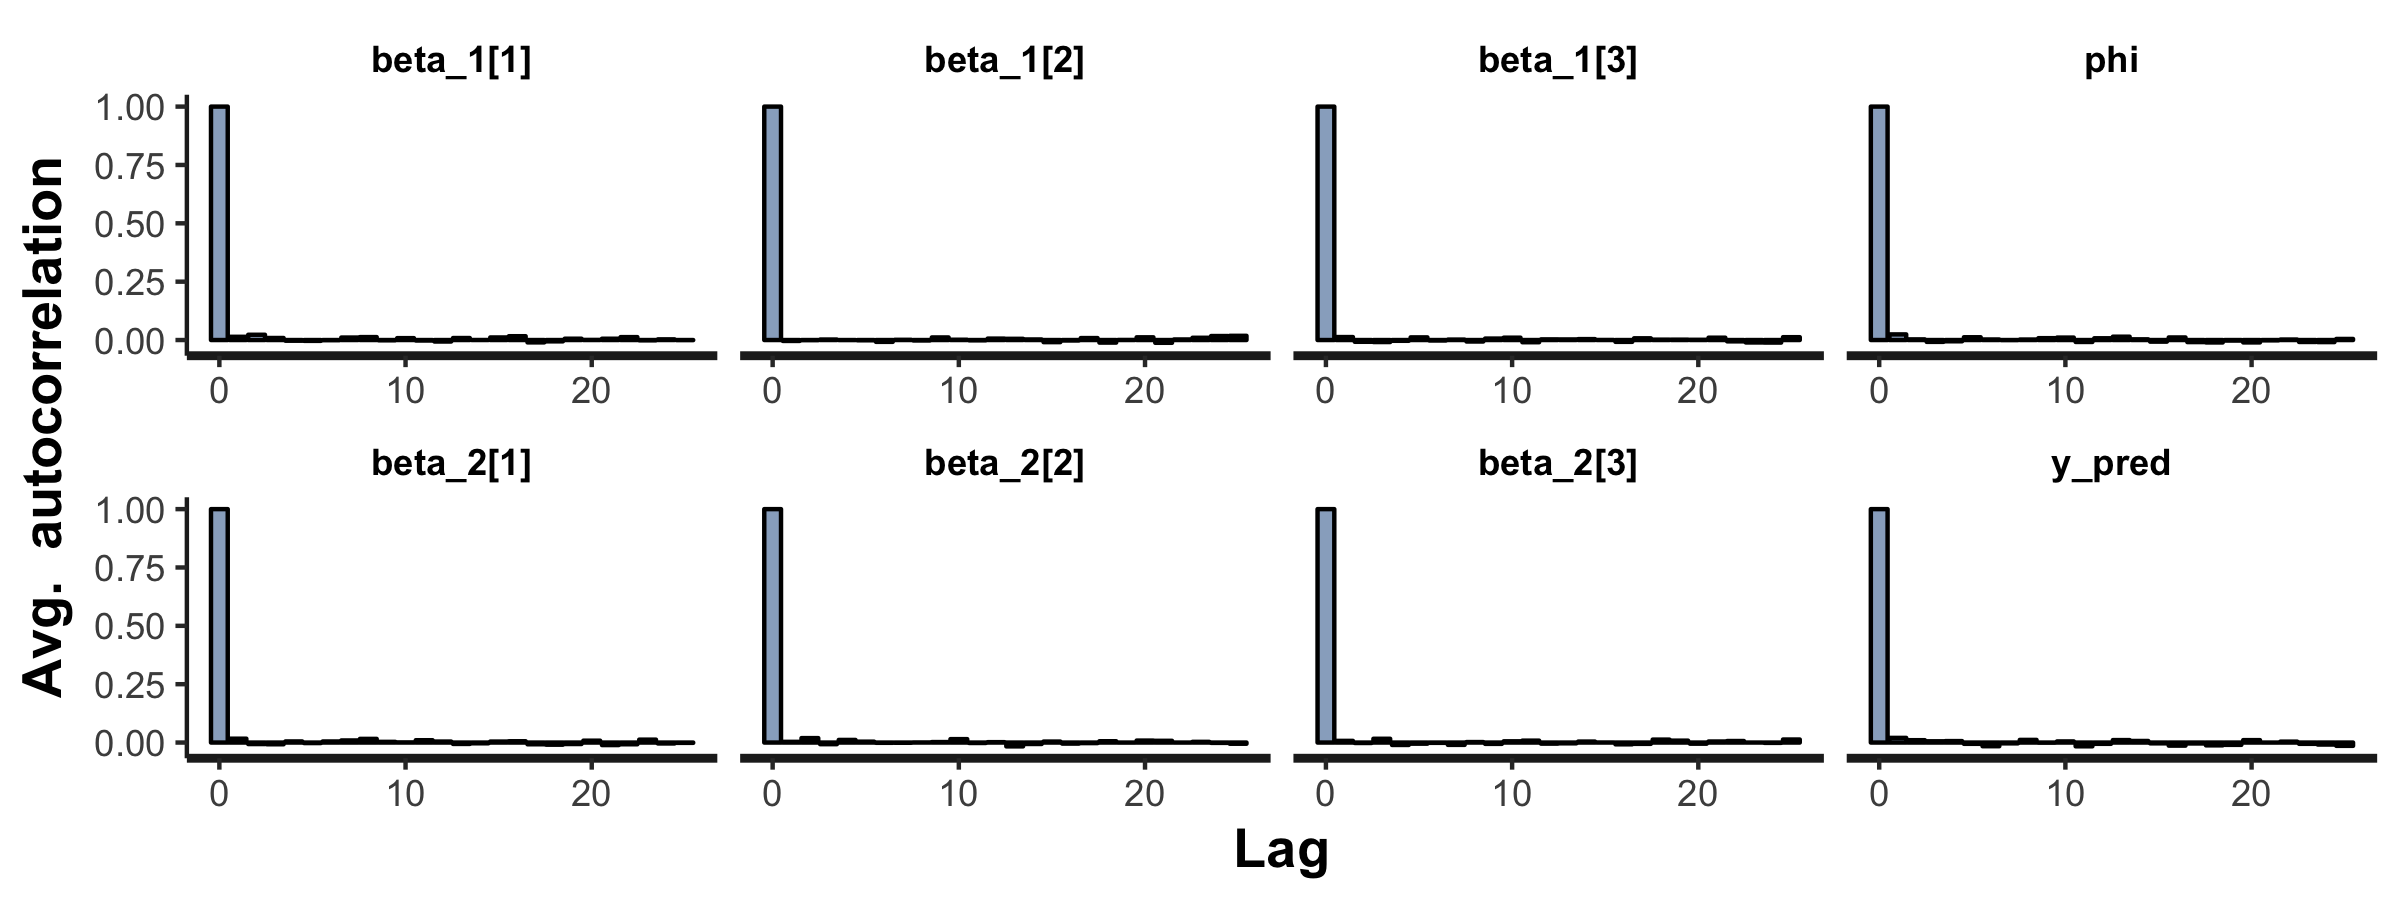
\includegraphics[width=16cm]{hier_2pars_ac.png}
\end{figure}

\newpage
\subsubsection*{van Genuchten model}
\begin{figure}[ht!]
\centering
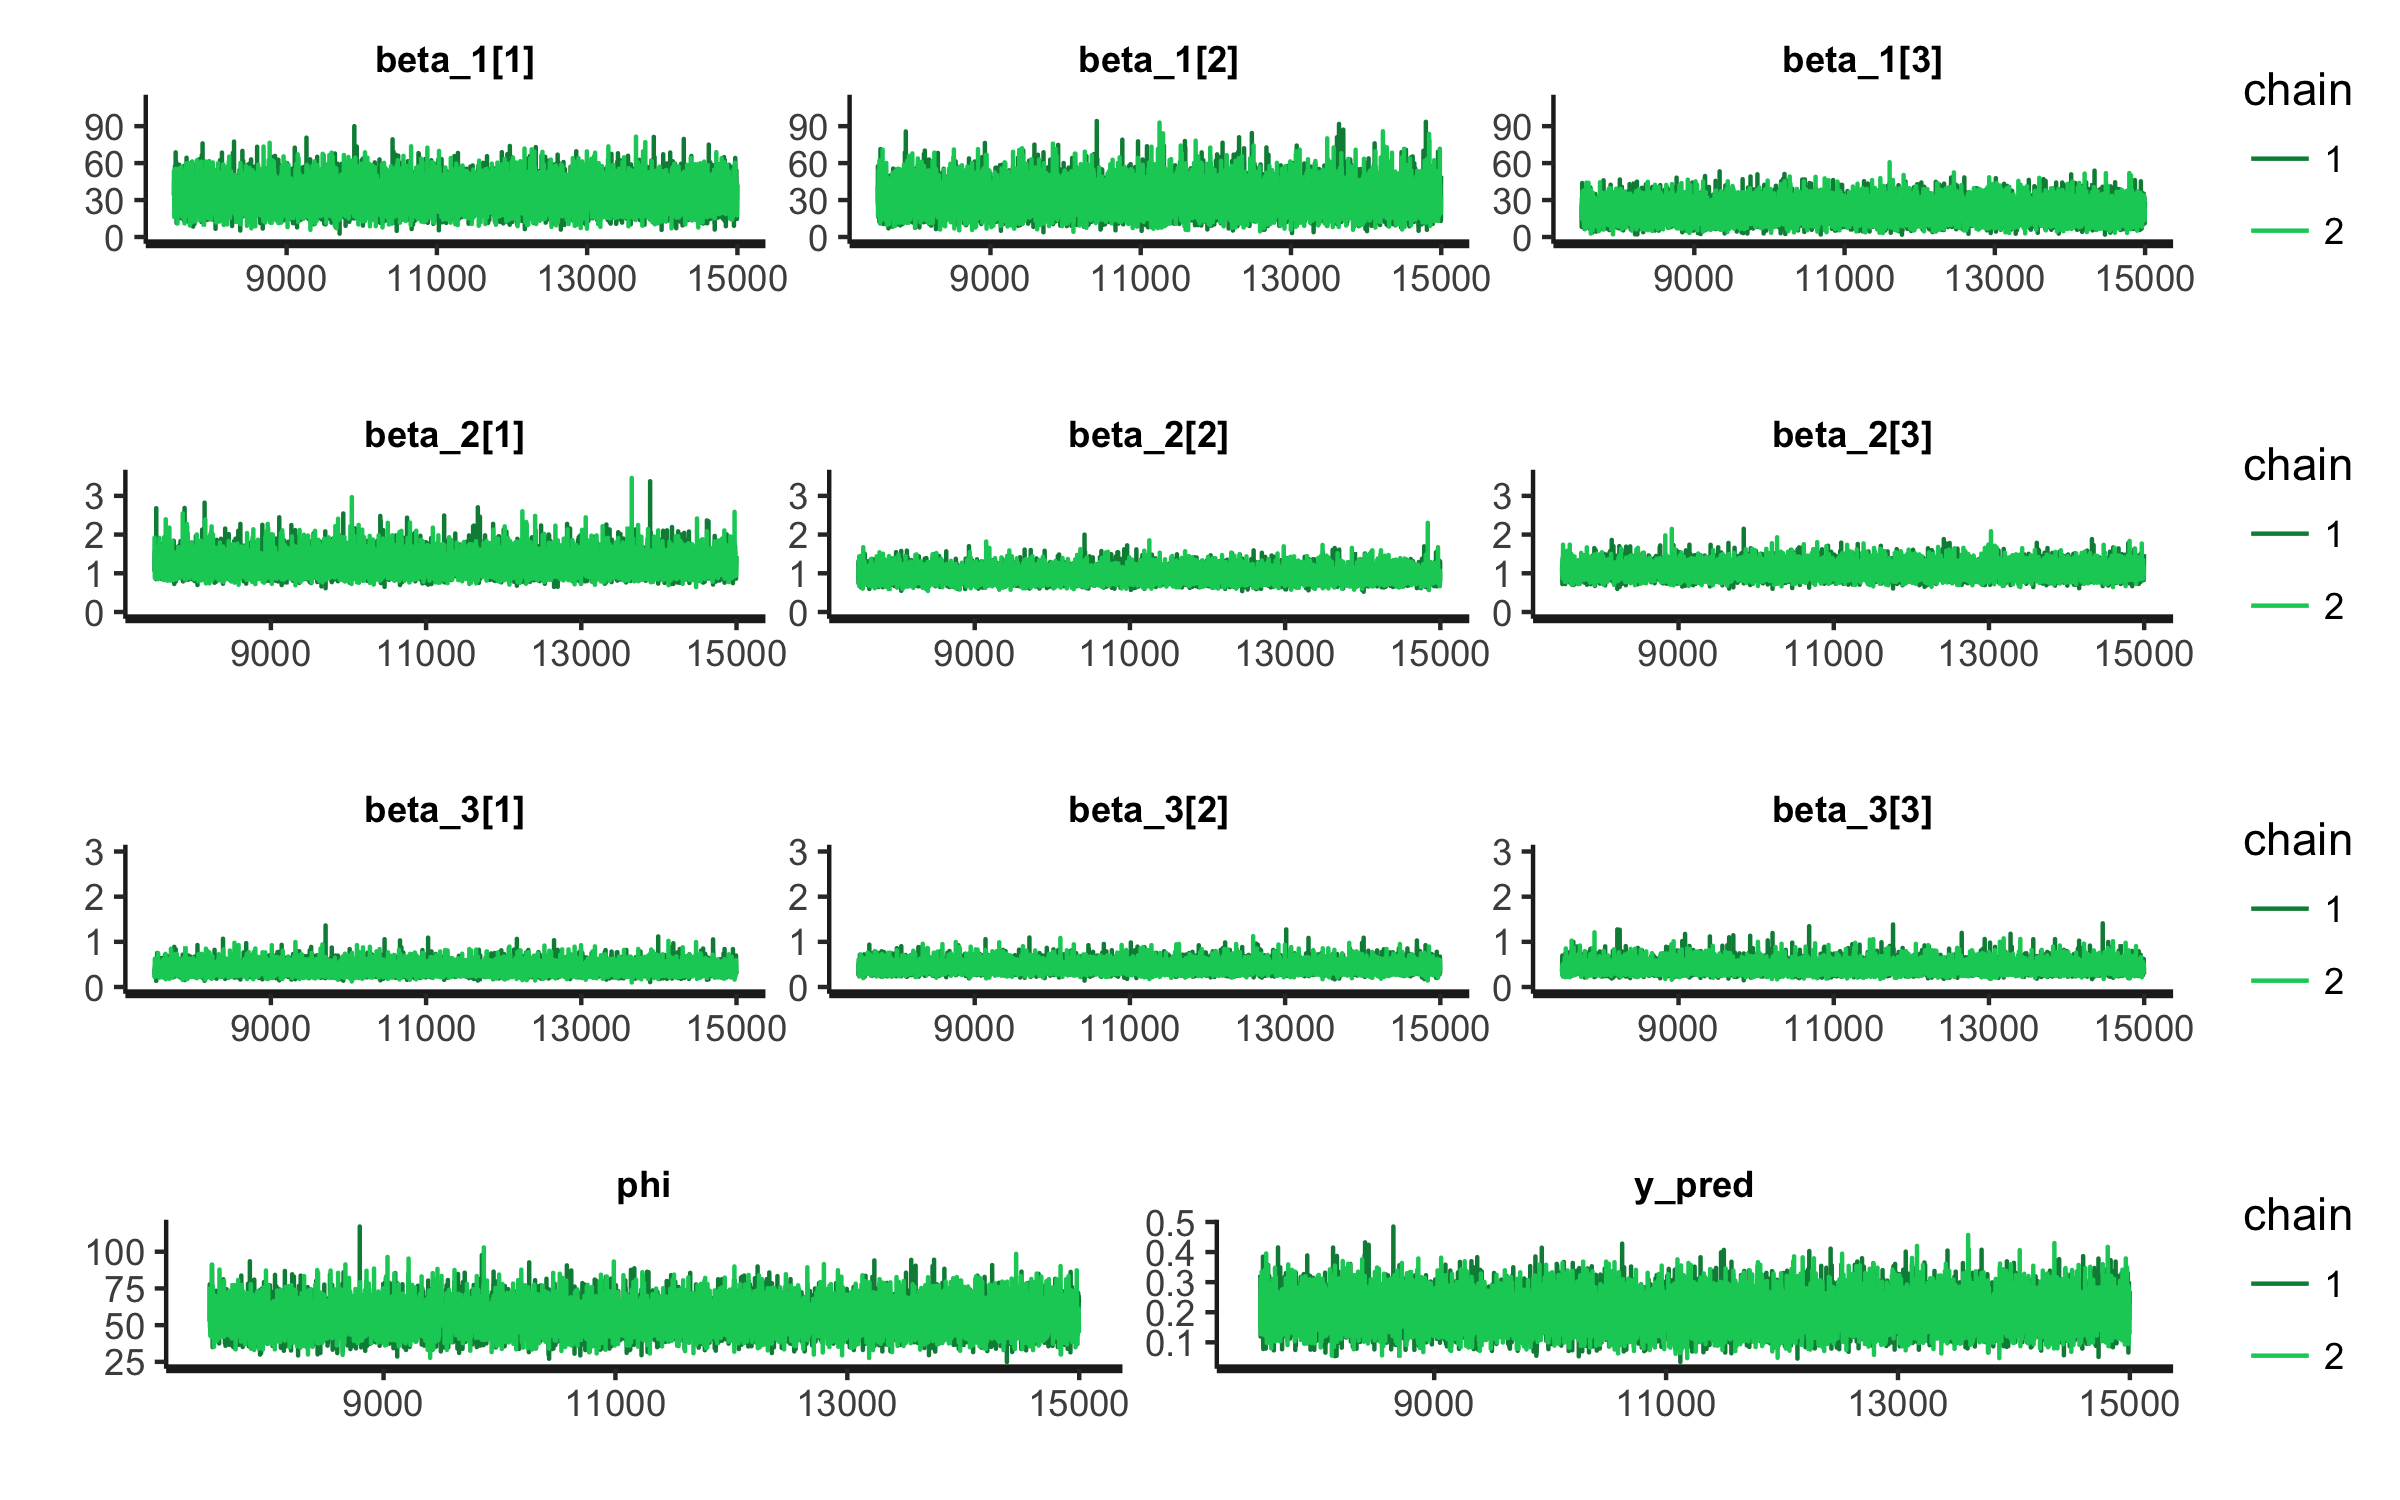
\includegraphics[width=16cm]{hier_3pars_trace.png}
\end{figure}

\begin{figure}[ht!]
\centering
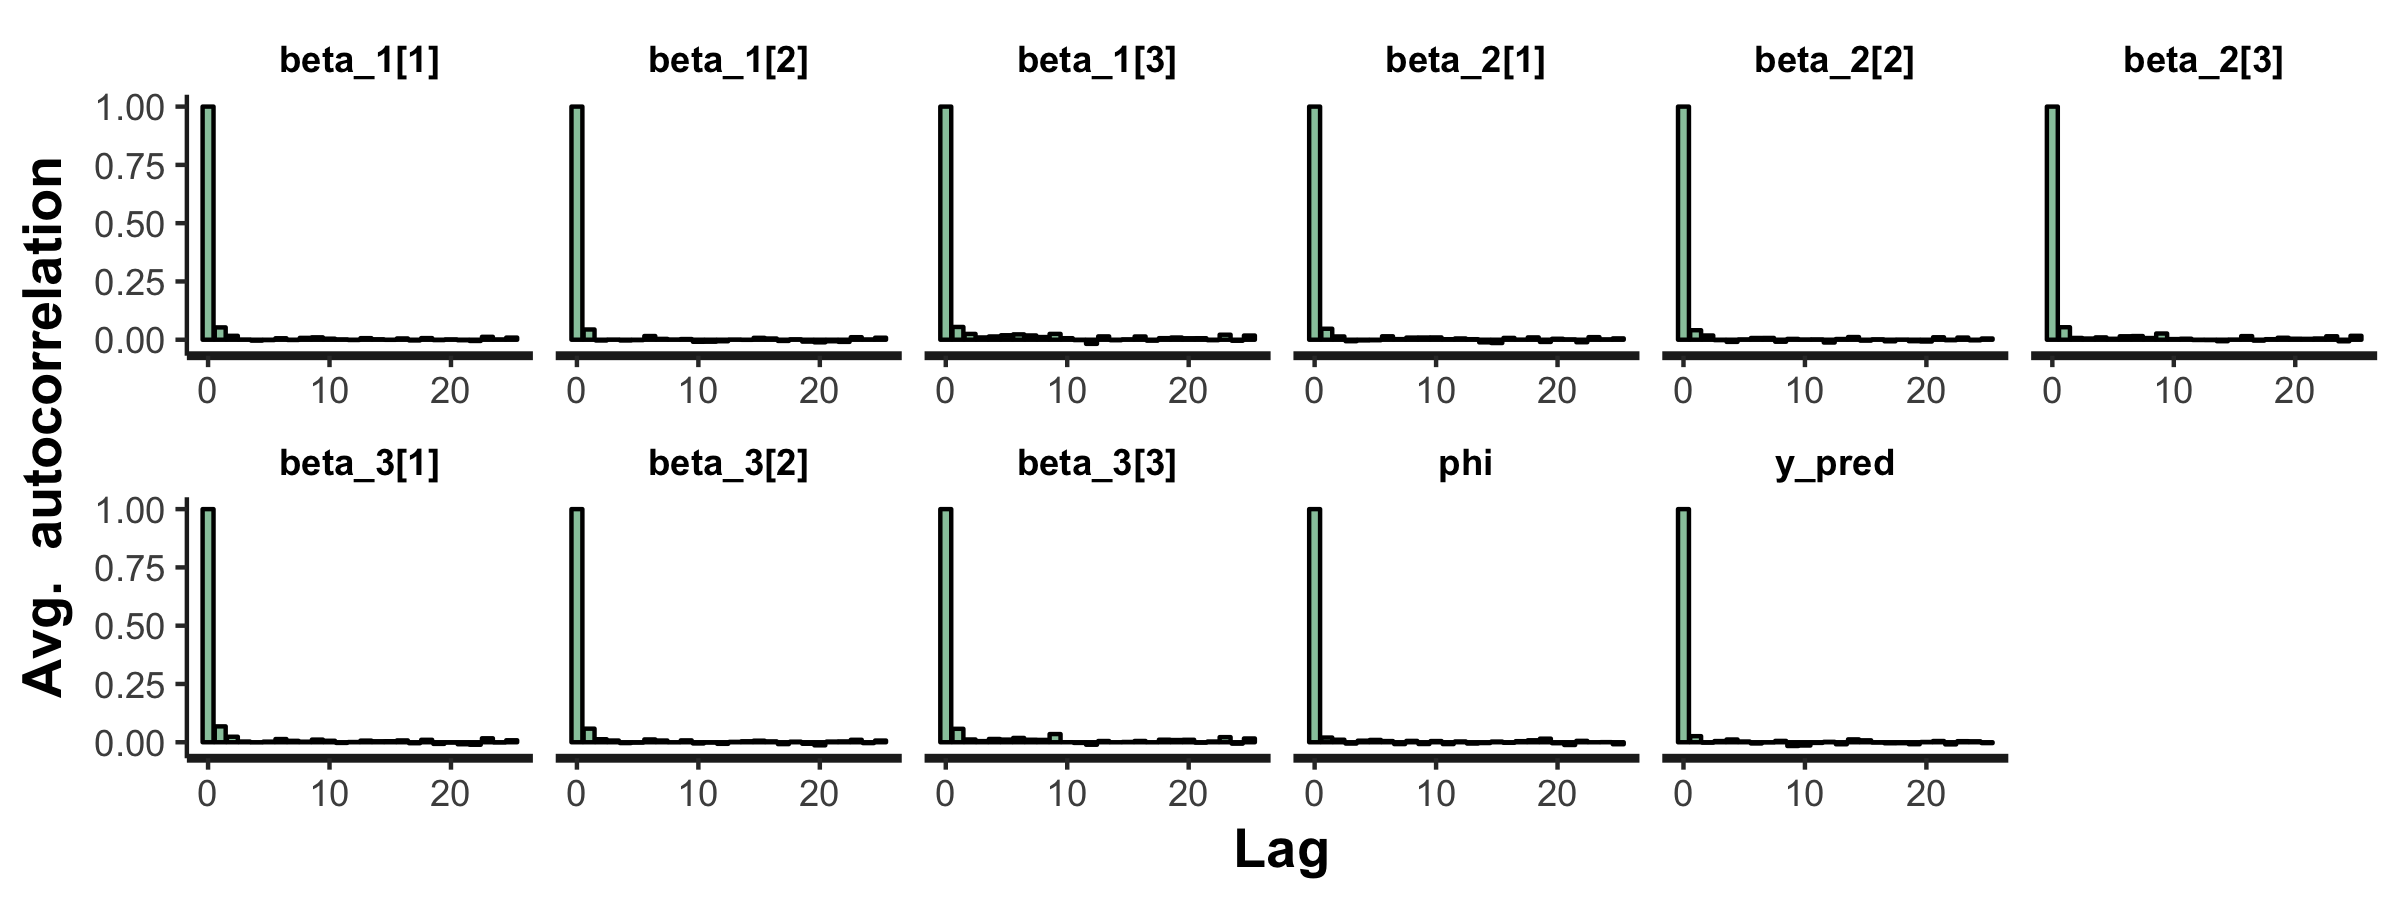
\includegraphics[width=16cm]{hier_3pars_ac.png}
\end{figure}

\begin{figure}[ht!]
\centering
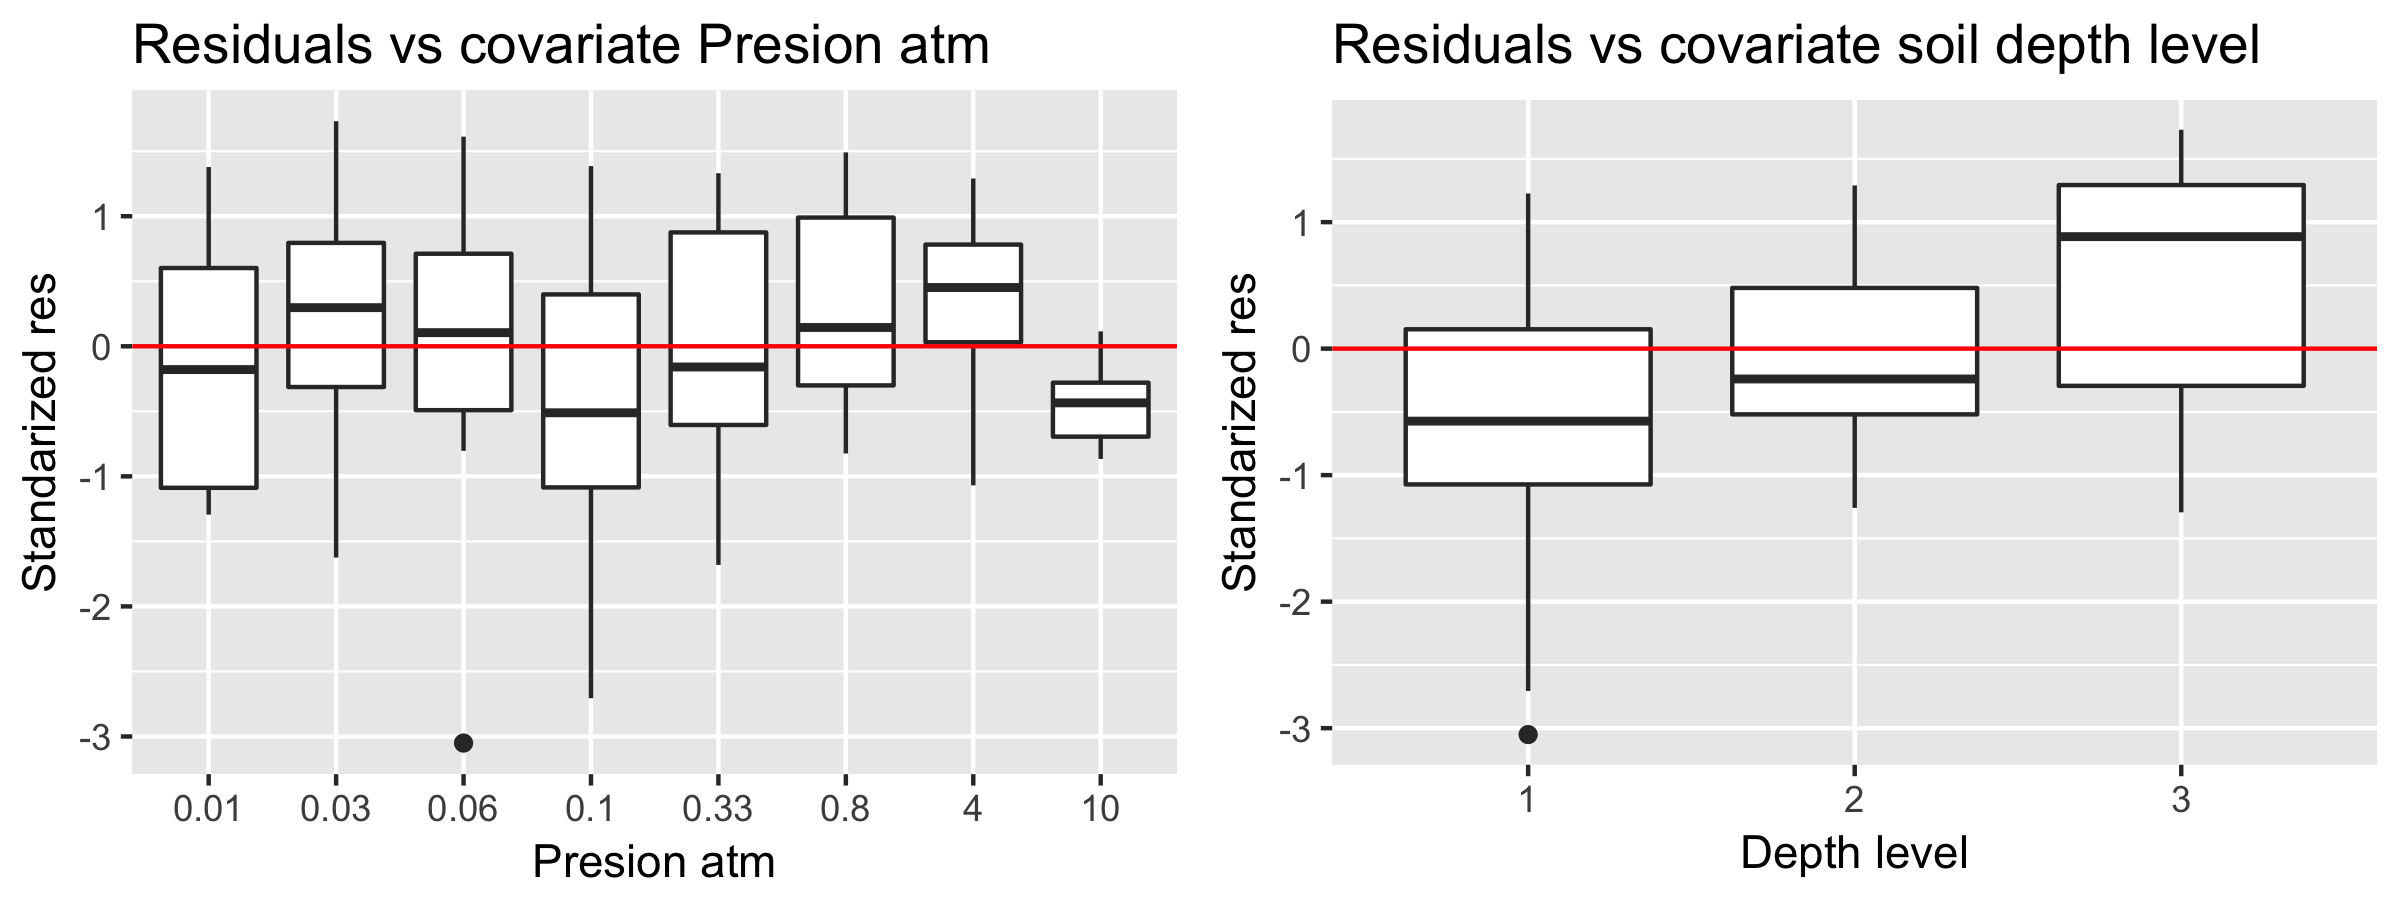
\includegraphics[width=13cm]{residuals.png}
\end{figure}

\newpage
\section{Code}
\subsection*{Hierarchical-effects model - van Genuchten}
As the modification for the Gardner's model is trivial, just the van Genuchten code is provided for each of the three models. 
\begin{lstlisting}
data {
    int<lower=0> n_tot;
    int<lower=0> Depth[n_tot];
    vector<lower=0>[n_tot] x; # Rregressor x, (Atm)
    vector<lower=0>[n_tot] ymax;
    vector<lower=0>[n_tot] ymin;
    vector<lower=0>[n_tot] y;
    int<lower=0> x_ind [n_tot]; # A new variable vas added to indicate the level of regressor x (from 1 to 8)
    int<lower=0> x_new; # New data
    int<lower=0> Depth_new; # New data
}
transformed data {
    vector<lower=0, upper=1>[n_tot] y_hat;
    for (i in  1:n_tot)
      y_hat[i] = (y[i]-ymin[i])*pow(ymax[i]-ymin[i], -1); # Reescaled dependent variable
}
parameters {
    real<lower=0> beta_1[3];
    real<lower=0> beta_2[3];
    real<lower=0> beta_3[3];
    real<lower=0> phi;
    real<lower=0> alpha1;
    real<lower=0> alpha2;
    real<lower=0> alpha3;
    real<lower=0> beta1;
    real<lower=0> beta2;
    real<lower=0> beta3;
    real<lower=0> y_pred; # variable of prediction given x_new and depth_new
    real<lower=0, upper= 1> fitted[24]; # fitted values for the model
}
transformed parameters {
    vector<lower=0>[24] mu; # in total 24 mu's (8 levels of regressor x, and 3 levels of depth)
    vector<lower=0>[24] sigma2;
    real<lower=0> mu_pred;
    real<lower=0> sigma2_pred;
    for (j in 0: 2){
      for (i in 1:8){
        mu[j*8+i] = 1*pow((1 + pow(beta_1[Depth[j*24+i]] * x[i], beta_2[Depth[j*24+i]])),-beta_3[Depth[j*24+i]]);
        sigma2[j*8+i] = mu[j*8+i] .*(1-mu[j*8+i]).*pow((phi+1), -1);
      }
    }
    mu_pred = 1*pow((1 + pow(beta_1[Depth_new] * x_new, beta_2[Depth_new])),-beta_3[Depth_new]);
    sigma2_pred = mu_pred .*(1-mu_pred).*pow((phi+1), -1);
}
model {
  for ( i in 0:2 ){ # total 3*3*8 observations correspond to depth 1
    for ( j in 0:2 ){ # first 3*8 observations correspond to depth 1
      for ( k in 1:8 ){ # level of regressor x, takes 8 values (same mean for each level)
        y_hat[i*24+j*8+k] ~ beta(mu[i*8+x_ind[k]].*phi, (1-mu[i*8+x_ind[k]]).*phi); # van Genuchten model
      }
    }
  }
  for( i in 1:3){ # hierarchical model
    beta_1[i] ~ gamma(alpha1, beta1);
    beta_2[i] ~ gamma(alpha2, beta2);
    beta_3[i] ~ gamma(alpha3, beta3);
  }
  alpha1 ~ gamma(0.01, 0.01); 
  alpha2 ~ gamma(0.01, 0.01);
  alpha3 ~ gamma(0.01, 0.01);
  beta1 ~ gamma(0.01, 0.01);
  beta2 ~ gamma(0.01, 0.01);
  beta3 ~ gamma(0.01, 0.01);
  phi ~ gamma(.01, .01);
  y_pred ~ beta(mu_pred*phi, (1-mu_pred)*phi); # prediction distribution
  for (j in 0: 2){
      for (i in 1:8){
        fitted[j*8+i] ~ beta(mu[j*8+i]*phi, (1-mu[j*8+i])*phi); # fitted values
      }
  }
}
generated quantities{
  vector[n_tot] log_lik; # pointwise log likelihood 
  vector[n_tot] stres; # standarized residuals
  for ( i in 0:2 ){
    for ( j in 0:2 ){
      for ( k in 1:8 ){
        log_lik[i*24+j*8+k] = beta_lpdf(y_hat[i*24+j*8+k] | mu[i*8+x_ind[k]].*phi, (1-mu[i*8+x_ind[k]]).*phi);
        stres[i*24+j*8+k] = (y_hat[i*24+j*8+k]-mu[i*8+x_ind[k]]*pow(sigma2[i*8+x_ind[k]], -0.5));
      }
    }
  }
}
\end{lstlisting}

\subsection*{Independent-effects model - van Genuchten}
\begin{lstlisting}
data {
    int<lower=0> n_tot;
    int<lower=0> Depth[n_tot];
    vector<lower=0>[n_tot] x;
    vector<lower=0>[n_tot] ymax;
    vector<lower=0>[n_tot] ymin;
    vector<lower=0>[n_tot] y;
    int<lower=0> x_ind [n_tot];
    int<lower=0> x_new;
    int<lower=0> Depth_new;
}

transformed data {
    vector<lower=0, upper=1>[n_tot] y_hat;
    for (i in  1:n_tot)
      y_hat[i] = (y[i]-ymin[i])*pow(ymax[i]-ymin[i], -1);
}

parameters {
    real<lower=0> beta_1[3];
    real<lower=0> beta_2[3];
    real<lower=0> beta_3[3];
    real<lower=0> phi;
    real<lower=0> y_pred;
    real<lower=0, upper= 1> fitted[24];
}

transformed parameters {
    vector<lower=0>[24] mu;
    vector<lower=0>[24] sigma2;
    real<lower=0> mu_pred;
    real<lower=0> sigma2_pred;
    
    for (j in 0: 2){
      for (i in 1:8){
        mu[j*8+i] = 1*pow((1 + pow(beta_1[Depth[j*24+i]] * x[i], beta_2[Depth[j*24+i]])),-beta_3[Depth[j*24+i]]);
        sigma2[j*8+i] = mu[j*8+i] .*(1-mu[j*8+i]).*pow((phi+1), -1);
      }
    }
    mu_pred = 1*pow((1 + pow(beta_1[Depth_new] * x_new, beta_2[Depth_new])),-beta_3[Depth_new]);
    sigma2_pred = mu_pred .*(1-mu_pred).*pow((phi+1), -1);
}

model {
  for ( i in 0:2 ){
    for ( j in 0:2 ){
      for ( k in 1:8 ){
        y_hat[i*24+j*8+k] ~ beta(mu[i*8+x_ind[k]].*phi, (1-mu[i*8+x_ind[k]]).*phi);
      }
    }
  }
  for( i in 1:3){
    beta_1[i] ~ gamma(.01, .01);
    beta_2[i] ~ gamma(.01, .01);
    beta_3[i] ~ gamma(.01, .01);
  }
  phi ~ gamma(.01, .01);
  y_pred ~ beta(mu_pred*phi, (1-mu_pred)*phi);
  
  for (j in 0: 2){
      for (i in 1:8){
        fitted[j*8+i] ~ beta(mu[j*8+i]*phi, (1-mu[j*8+i])*phi);
      }
  }
}

generated quantities{
  vector[n_tot] log_lik;
  for ( i in 0:2 ){
    for ( j in 0:2 ){
      for ( k in 1:8 ){
        log_lik[i*24+j*8+k] = beta_lpdf(y_hat[i*24+j*8+k] | mu[i*8+x_ind[k]].*phi, (1-mu[i*8+x_ind[k]]).*phi);
      }
    }
  }
}
\end{lstlisting}

\subsection*{Pooled-effects model - van Genuchten}
\begin{lstlisting}
data {
    int<lower=0> n_tot;
    vector<lower=0>[n_tot] Depth;
    vector<lower=0>[n_tot] x;
    vector<lower=0>[n_tot] ymax;
    vector<lower=0>[n_tot] ymin;
    vector<lower=0>[n_tot] y;
    int<lower=0> x_ind [n_tot];
    int<lower=0> x_new;
    int<lower=0> Depth_new;
}

transformed data {
    vector<lower=0, upper=1>[n_tot] y_hat;
    for (i in  1:n_tot)
      y_hat[i] = (y[i]-ymin[i])*pow(ymax[i]-ymin[i], -1);
}

parameters {
    real<lower=0> beta_1;
    real<lower=0> beta_2;
    real<lower=0> beta_3;
    real<lower=0> phi;
    real<lower=0> y_pred;
    real<lower=0, upper= 1> fitted[8];
}

transformed parameters {
    vector<lower=0>[8] mu;
    vector<lower=0>[8] sigma2;
    real<lower=0> mu_pred;
    real<lower=0> sigma2_pred;
    
    for (i in 1:8){
      mu[i] = 1*pow((1 + pow(beta_1 * x[i], beta_2)),-beta_3);
      sigma2[i] = mu[i] .*(1-mu[i]).*pow((phi+1), -1);
    }
    mu_pred = 1*pow((1 + pow(beta_1 * x_new, beta_2)),-beta_3);
    sigma2_pred = mu_pred .*(1-mu_pred).*pow((phi+1), -1);
}

model {
  for (i in 1:72){
    y_hat[i] ~ beta(mu[x_ind[i]].*phi, (1-mu[x_ind[i]]).*phi);
  }
  beta_1 ~ gamma(.01, .01);
  beta_2 ~ gamma(.01, .01);
  beta_3 ~ gamma(.01, .01);
  phi ~ gamma(.01, .01);
  
  y_pred ~ beta(mu_pred*phi, (1-mu_pred)*phi);
  
  for (i in 1:8){
      fitted[i] ~ beta(mu[i]*phi, (1-mu[i])*phi);
  }
}

generated quantities{
  vector[n_tot] log_lik;
  for ( i in 1:72 ){
        log_lik[i] = beta_lpdf(y_hat[i] | mu[x_ind[i]].*phi, (1-mu[x_ind[i]]).*phi);
  }
}
\end{lstlisting}


\bibliographystyle{apacite}
\bibliography{ref}
\end{document}
